% Options for packages loaded elsewhere
\PassOptionsToPackage{unicode}{hyperref}
\PassOptionsToPackage{hyphens}{url}
%
\documentclass[
]{book}
\usepackage{amsmath,amssymb}
\usepackage{lmodern}
\usepackage{iftex}
\ifPDFTeX
  \usepackage[T1]{fontenc}
  \usepackage[utf8]{inputenc}
  \usepackage{textcomp} % provide euro and other symbols
\else % if luatex or xetex
  \usepackage{unicode-math}
  \defaultfontfeatures{Scale=MatchLowercase}
  \defaultfontfeatures[\rmfamily]{Ligatures=TeX,Scale=1}
\fi
% Use upquote if available, for straight quotes in verbatim environments
\IfFileExists{upquote.sty}{\usepackage{upquote}}{}
\IfFileExists{microtype.sty}{% use microtype if available
  \usepackage[]{microtype}
  \UseMicrotypeSet[protrusion]{basicmath} % disable protrusion for tt fonts
}{}
\makeatletter
\@ifundefined{KOMAClassName}{% if non-KOMA class
  \IfFileExists{parskip.sty}{%
    \usepackage{parskip}
  }{% else
    \setlength{\parindent}{0pt}
    \setlength{\parskip}{6pt plus 2pt minus 1pt}}
}{% if KOMA class
  \KOMAoptions{parskip=half}}
\makeatother
\usepackage{xcolor}
\usepackage{color}
\usepackage{fancyvrb}
\newcommand{\VerbBar}{|}
\newcommand{\VERB}{\Verb[commandchars=\\\{\}]}
\DefineVerbatimEnvironment{Highlighting}{Verbatim}{commandchars=\\\{\}}
% Add ',fontsize=\small' for more characters per line
\usepackage{framed}
\definecolor{shadecolor}{RGB}{248,248,248}
\newenvironment{Shaded}{\begin{snugshade}}{\end{snugshade}}
\newcommand{\AlertTok}[1]{\textcolor[rgb]{0.94,0.16,0.16}{#1}}
\newcommand{\AnnotationTok}[1]{\textcolor[rgb]{0.56,0.35,0.01}{\textbf{\textit{#1}}}}
\newcommand{\AttributeTok}[1]{\textcolor[rgb]{0.77,0.63,0.00}{#1}}
\newcommand{\BaseNTok}[1]{\textcolor[rgb]{0.00,0.00,0.81}{#1}}
\newcommand{\BuiltInTok}[1]{#1}
\newcommand{\CharTok}[1]{\textcolor[rgb]{0.31,0.60,0.02}{#1}}
\newcommand{\CommentTok}[1]{\textcolor[rgb]{0.56,0.35,0.01}{\textit{#1}}}
\newcommand{\CommentVarTok}[1]{\textcolor[rgb]{0.56,0.35,0.01}{\textbf{\textit{#1}}}}
\newcommand{\ConstantTok}[1]{\textcolor[rgb]{0.00,0.00,0.00}{#1}}
\newcommand{\ControlFlowTok}[1]{\textcolor[rgb]{0.13,0.29,0.53}{\textbf{#1}}}
\newcommand{\DataTypeTok}[1]{\textcolor[rgb]{0.13,0.29,0.53}{#1}}
\newcommand{\DecValTok}[1]{\textcolor[rgb]{0.00,0.00,0.81}{#1}}
\newcommand{\DocumentationTok}[1]{\textcolor[rgb]{0.56,0.35,0.01}{\textbf{\textit{#1}}}}
\newcommand{\ErrorTok}[1]{\textcolor[rgb]{0.64,0.00,0.00}{\textbf{#1}}}
\newcommand{\ExtensionTok}[1]{#1}
\newcommand{\FloatTok}[1]{\textcolor[rgb]{0.00,0.00,0.81}{#1}}
\newcommand{\FunctionTok}[1]{\textcolor[rgb]{0.00,0.00,0.00}{#1}}
\newcommand{\ImportTok}[1]{#1}
\newcommand{\InformationTok}[1]{\textcolor[rgb]{0.56,0.35,0.01}{\textbf{\textit{#1}}}}
\newcommand{\KeywordTok}[1]{\textcolor[rgb]{0.13,0.29,0.53}{\textbf{#1}}}
\newcommand{\NormalTok}[1]{#1}
\newcommand{\OperatorTok}[1]{\textcolor[rgb]{0.81,0.36,0.00}{\textbf{#1}}}
\newcommand{\OtherTok}[1]{\textcolor[rgb]{0.56,0.35,0.01}{#1}}
\newcommand{\PreprocessorTok}[1]{\textcolor[rgb]{0.56,0.35,0.01}{\textit{#1}}}
\newcommand{\RegionMarkerTok}[1]{#1}
\newcommand{\SpecialCharTok}[1]{\textcolor[rgb]{0.00,0.00,0.00}{#1}}
\newcommand{\SpecialStringTok}[1]{\textcolor[rgb]{0.31,0.60,0.02}{#1}}
\newcommand{\StringTok}[1]{\textcolor[rgb]{0.31,0.60,0.02}{#1}}
\newcommand{\VariableTok}[1]{\textcolor[rgb]{0.00,0.00,0.00}{#1}}
\newcommand{\VerbatimStringTok}[1]{\textcolor[rgb]{0.31,0.60,0.02}{#1}}
\newcommand{\WarningTok}[1]{\textcolor[rgb]{0.56,0.35,0.01}{\textbf{\textit{#1}}}}
\usepackage{longtable,booktabs,array}
\usepackage{calc} % for calculating minipage widths
% Correct order of tables after \paragraph or \subparagraph
\usepackage{etoolbox}
\makeatletter
\patchcmd\longtable{\par}{\if@noskipsec\mbox{}\fi\par}{}{}
\makeatother
% Allow footnotes in longtable head/foot
\IfFileExists{footnotehyper.sty}{\usepackage{footnotehyper}}{\usepackage{footnote}}
\makesavenoteenv{longtable}
\usepackage{graphicx}
\makeatletter
\def\maxwidth{\ifdim\Gin@nat@width>\linewidth\linewidth\else\Gin@nat@width\fi}
\def\maxheight{\ifdim\Gin@nat@height>\textheight\textheight\else\Gin@nat@height\fi}
\makeatother
% Scale images if necessary, so that they will not overflow the page
% margins by default, and it is still possible to overwrite the defaults
% using explicit options in \includegraphics[width, height, ...]{}
\setkeys{Gin}{width=\maxwidth,height=\maxheight,keepaspectratio}
% Set default figure placement to htbp
\makeatletter
\def\fps@figure{htbp}
\makeatother
\setlength{\emergencystretch}{3em} % prevent overfull lines
\providecommand{\tightlist}{%
  \setlength{\itemsep}{0pt}\setlength{\parskip}{0pt}}
\setcounter{secnumdepth}{5}
\usepackage{booktabs}
\usepackage{amsthm}
\makeatletter
\def\thm@space@setup{%
  \thm@preskip=8pt plus 2pt minus 4pt
  \thm@postskip=\thm@preskip
}
\makeatother
\ifLuaTeX
  \usepackage{selnolig}  % disable illegal ligatures
\fi
\usepackage[]{natbib}
\bibliographystyle{apalike}
\IfFileExists{bookmark.sty}{\usepackage{bookmark}}{\usepackage{hyperref}}
\IfFileExists{xurl.sty}{\usepackage{xurl}}{} % add URL line breaks if available
\urlstyle{same} % disable monospaced font for URLs
\hypersetup{
  pdftitle={Mastering Shiny Solutions},
  pdfauthor={The R4DS Online Learning Community},
  hidelinks,
  pdfcreator={LaTeX via pandoc}}

\title{Mastering Shiny Solutions}
\author{The R4DS Online Learning Community}
\date{(updated on 2023-02-08)}

\usepackage{amsthm}
\newtheorem{theorem}{Theorem}[chapter]
\newtheorem{lemma}{Lemma}[chapter]
\newtheorem{corollary}{Corollary}[chapter]
\newtheorem{proposition}{Proposition}[chapter]
\newtheorem{conjecture}{Conjecture}[chapter]
\theoremstyle{definition}
\newtheorem{definition}{Definition}[chapter]
\theoremstyle{definition}
\newtheorem{example}{Example}[chapter]
\theoremstyle{definition}
\newtheorem{exercise}{Exercise}[chapter]
\theoremstyle{definition}
\newtheorem{hypothesis}{Hypothesis}[chapter]
\theoremstyle{remark}
\newtheorem*{remark}{Remark}
\newtheorem*{solution}{Solution}
\begin{document}
\maketitle

{
\setcounter{tocdepth}{1}
\tableofcontents
}
\hypertarget{welcome}{%
\chapter*{Welcome}\label{welcome}}
\addcontentsline{toc}{chapter}{Welcome}

This book offers solutions to the exercises from Hadley Wickham's book \href{https://mastering-shiny.org/}{Mastering Shiny}. It is a work in progress and under active development. The code for this book can be found on \href{https://github.com/r4ds/mastering_shiny_book_solutions}{GitHub}. Your PRs and suggestions are very welcome.

\hypertarget{note-boxes}{%
\section*{Note Boxes}\label{note-boxes}}
\addcontentsline{toc}{section}{Note Boxes}

We use three different types of boxes throughout the book.

This ``note'' box denotes we were either unclear what the exercise was asking or have follow up questions.

This ``TODO'' box denotes that the exercises in the chapter have either partial solutions or have yet to be reviewed.

\hypertarget{license}{%
\section*{License}\label{license}}
\addcontentsline{toc}{section}{License}

This work by Maya Gans and Marly Gotti is licensed under a Creative Commons Attribution-NonCommercial-ShareAlike 4.0 International License

\hypertarget{acknowledgements}{%
\section*{Acknowledgements}\label{acknowledgements}}
\addcontentsline{toc}{section}{Acknowledgements}

\hypertarget{preface}{%
\chapter{Preface}\label{preface}}

There are no exercises in this chapter.

\hypertarget{your-first-shiny-app}{%
\chapter{Your First Shiny App}\label{your-first-shiny-app}}

\hypertarget{exercise-2.8.1}{%
\subsection*{Exercise 2.8.1}\label{exercise-2.8.1}}
\addcontentsline{toc}{subsection}{Exercise 2.8.1}

Create an app that greets the user by name. You don't know all the functions
you need to do this yet, so I've included some lines of code below. Figure out
which lines you'll use and then copy and paste them into the right place in a
Shiny app.

\begin{Shaded}
\begin{Highlighting}[]
\FunctionTok{textInput}\NormalTok{(}\StringTok{"name"}\NormalTok{, }\StringTok{"What\textquotesingle{}s your name?"}\NormalTok{)}
\FunctionTok{renderText}\NormalTok{(\{}
  \FunctionTok{paste0}\NormalTok{(}\StringTok{"Hello "}\NormalTok{, input}\SpecialCharTok{$}\NormalTok{name)}
\NormalTok{\})}
\FunctionTok{numericInput}\NormalTok{(}\StringTok{"age"}\NormalTok{, }\StringTok{"How old are you?"}\NormalTok{)}
\FunctionTok{textOutput}\NormalTok{(}\StringTok{"greeting"}\NormalTok{)}
\FunctionTok{tableOutput}\NormalTok{(}\StringTok{"mortgage"}\NormalTok{)}
\FunctionTok{renderPlot}\NormalTok{(}\StringTok{"histogram"}\NormalTok{, \{}
  \FunctionTok{hist}\NormalTok{(}\FunctionTok{rnorm}\NormalTok{(}\DecValTok{1000}\NormalTok{))}
\NormalTok{\}, }\AttributeTok{res =} \DecValTok{96}\NormalTok{)}
\end{Highlighting}
\end{Shaded}

\begin{solution}
\leavevmode

\hypertarget{solution}{%
\subsubsection*{Solution}\label{solution}}
\addcontentsline{toc}{subsubsection}{Solution}

In the UI, we will need a \texttt{textInput} for the user to input text, and
a \texttt{textOutput} to output any custom text to the app. The corresponding server
function to \texttt{textOutput} is \texttt{renderText}, which we can use to compose the
output element we've named ``greeting''.

\begin{Shaded}
\begin{Highlighting}[]
\FunctionTok{library}\NormalTok{(shiny)}

\NormalTok{ui }\OtherTok{\textless{}{-}} \FunctionTok{fluidPage}\NormalTok{(}
  \FunctionTok{textInput}\NormalTok{(}\StringTok{"name"}\NormalTok{, }\StringTok{"What\textquotesingle{}s your name?"}\NormalTok{),}
  \FunctionTok{textOutput}\NormalTok{(}\StringTok{"greeting"}\NormalTok{)}
\NormalTok{)}

\NormalTok{server }\OtherTok{\textless{}{-}} \ControlFlowTok{function}\NormalTok{(input, output, session) \{}
\NormalTok{  output}\SpecialCharTok{$}\NormalTok{greeting }\OtherTok{\textless{}{-}} \FunctionTok{renderText}\NormalTok{(\{}
    \FunctionTok{paste0}\NormalTok{(}\StringTok{"Hello "}\NormalTok{, input}\SpecialCharTok{$}\NormalTok{name)}
\NormalTok{  \})}
\NormalTok{\}}

\FunctionTok{shinyApp}\NormalTok{(ui, server)}
\end{Highlighting}
\end{Shaded}

\end{solution}

\hypertarget{exercise-2.8.2}{%
\section*{Exercise 2.8.2}\label{exercise-2.8.2}}
\addcontentsline{toc}{section}{Exercise 2.8.2}

Suppose your friend wants to design an app that allows the user to set a number
(\texttt{x}) between 1 and 50, and displays the result of multiplying this number by
5. This is their first attempt:

\begin{Shaded}
\begin{Highlighting}[]
\NormalTok{ui }\OtherTok{\textless{}{-}} \FunctionTok{fluidPage}\NormalTok{(}
  \FunctionTok{sliderInput}\NormalTok{(}\StringTok{"x"}\NormalTok{, }\AttributeTok{label =} \StringTok{"If x is"}\NormalTok{, }\AttributeTok{min =} \DecValTok{1}\NormalTok{, }\AttributeTok{max =} \DecValTok{50}\NormalTok{, }\AttributeTok{value =} \DecValTok{30}\NormalTok{),}
  \StringTok{"then x times 5 is"}\NormalTok{,}
  \FunctionTok{textOutput}\NormalTok{(}\StringTok{"product"}\NormalTok{)}
\NormalTok{)}

\NormalTok{server }\OtherTok{\textless{}{-}} \ControlFlowTok{function}\NormalTok{(input, output, session) \{}
\NormalTok{  output}\SpecialCharTok{$}\NormalTok{product }\OtherTok{\textless{}{-}} \FunctionTok{renderText}\NormalTok{(\{ }
\NormalTok{    x }\SpecialCharTok{*} \DecValTok{5}
\NormalTok{  \})}
\NormalTok{\}}
\end{Highlighting}
\end{Shaded}

But unfortunately it has an error:

\begin{figure}
\centering
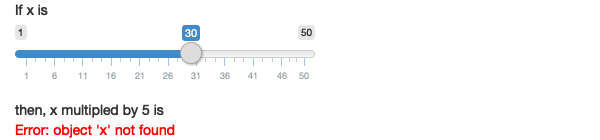
\includegraphics{images/ex-x-times-5.png}
\caption{placeholder}
\end{figure}

Can you help them find and correct the error?

\begin{solution}
\leavevmode

\hypertarget{solution-1}{%
\subsubsection*{Solution}\label{solution-1}}
\addcontentsline{toc}{subsubsection}{Solution}

The error here arises because on the server side we need to write \texttt{input\$x}
rather than \texttt{x}. By writing \texttt{x}, we are looking for element \texttt{x} which doesn't
exist in the Shiny environment; \texttt{x} only exists within the read-only object
\texttt{input}.

\begin{Shaded}
\begin{Highlighting}[]
\FunctionTok{library}\NormalTok{(shiny)}

\NormalTok{ui }\OtherTok{\textless{}{-}} \FunctionTok{fluidPage}\NormalTok{(}
  \FunctionTok{sliderInput}\NormalTok{(}\StringTok{"x"}\NormalTok{, }\AttributeTok{label =} \StringTok{"If x is"}\NormalTok{, }\AttributeTok{min =} \DecValTok{1}\NormalTok{, }\AttributeTok{max =} \DecValTok{50}\NormalTok{, }\AttributeTok{value =} \DecValTok{30}\NormalTok{),}
  \StringTok{"then x times 5 is"}\NormalTok{,}
  \FunctionTok{textOutput}\NormalTok{(}\StringTok{"product"}\NormalTok{)}
\NormalTok{)}

\NormalTok{server }\OtherTok{\textless{}{-}} \ControlFlowTok{function}\NormalTok{(input, output, session) \{}
\NormalTok{  output}\SpecialCharTok{$}\NormalTok{product }\OtherTok{\textless{}{-}} \FunctionTok{renderText}\NormalTok{(\{ }
\NormalTok{    input}\SpecialCharTok{$}\NormalTok{x }\SpecialCharTok{*} \DecValTok{5}
\NormalTok{  \})}
\NormalTok{\}}

\FunctionTok{shinyApp}\NormalTok{(ui, server)}
\end{Highlighting}
\end{Shaded}

\end{solution}

\hypertarget{exercise-2.8.3}{%
\section*{Exercise 2.8.3}\label{exercise-2.8.3}}
\addcontentsline{toc}{section}{Exercise 2.8.3}

Extend the app from the previous exercise to allow the user to set the value of
the multiplier, \texttt{y}, so that the app yields the value of \texttt{x\ *\ y}. The final
result should look like this:

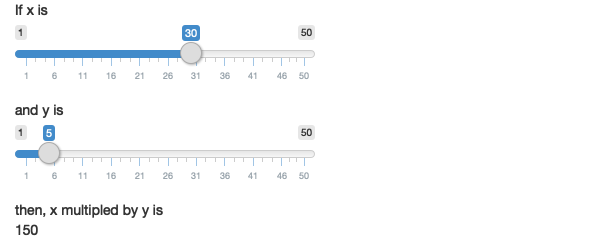
\includegraphics[width=8.33in]{./images/2.8.3}

\begin{solution}
\leavevmode

\hypertarget{solution-2}{%
\subsubsection*{Solution}\label{solution-2}}
\addcontentsline{toc}{subsubsection}{Solution}

Let us add another \texttt{sliderInput} with ID \texttt{y}, and use both \texttt{input\$x}
and \texttt{input\$y} to calculate \texttt{output\$product}.

\begin{Shaded}
\begin{Highlighting}[]
\FunctionTok{library}\NormalTok{(shiny)}

\NormalTok{ui }\OtherTok{\textless{}{-}} \FunctionTok{fluidPage}\NormalTok{(}
  \FunctionTok{sliderInput}\NormalTok{(}\StringTok{"x"}\NormalTok{, }\AttributeTok{label =} \StringTok{"If x is"}\NormalTok{, }\AttributeTok{min =} \DecValTok{1}\NormalTok{, }\AttributeTok{max =} \DecValTok{50}\NormalTok{, }\AttributeTok{value =} \DecValTok{30}\NormalTok{),}
  \FunctionTok{sliderInput}\NormalTok{(}\StringTok{"y"}\NormalTok{, }\AttributeTok{label =} \StringTok{"and y is"}\NormalTok{, }\AttributeTok{min =} \DecValTok{1}\NormalTok{, }\AttributeTok{max =} \DecValTok{50}\NormalTok{, }\AttributeTok{value =} \DecValTok{30}\NormalTok{),}
  \StringTok{"then x multiplied by y is"}\NormalTok{,}
  \FunctionTok{textOutput}\NormalTok{(}\StringTok{"product"}\NormalTok{)}
\NormalTok{)}

\NormalTok{server }\OtherTok{\textless{}{-}} \ControlFlowTok{function}\NormalTok{(input, output, session) \{}
\NormalTok{  output}\SpecialCharTok{$}\NormalTok{product }\OtherTok{\textless{}{-}} \FunctionTok{renderText}\NormalTok{(\{ }
\NormalTok{    input}\SpecialCharTok{$}\NormalTok{x }\SpecialCharTok{*}\NormalTok{ input}\SpecialCharTok{$}\NormalTok{y}
\NormalTok{  \})}
\NormalTok{\}}

\FunctionTok{shinyApp}\NormalTok{(ui, server)}
\end{Highlighting}
\end{Shaded}

\end{solution}

\hypertarget{exercise-2.8.4}{%
\section*{Exercise 2.8.4}\label{exercise-2.8.4}}
\addcontentsline{toc}{section}{Exercise 2.8.4}

Replace the UI and server components of your app from the previous exercise
with the UI and server components below, run the app, and describe the app's
functionality. Then reduce the duplication in the app by using a reactive
expression.

\begin{Shaded}
\begin{Highlighting}[]
\NormalTok{ui }\OtherTok{\textless{}{-}} \FunctionTok{fluidPage}\NormalTok{(}
  \FunctionTok{sliderInput}\NormalTok{(}\StringTok{"x"}\NormalTok{, }\StringTok{"If x is"}\NormalTok{, }\AttributeTok{min =} \DecValTok{1}\NormalTok{, }\AttributeTok{max =} \DecValTok{50}\NormalTok{, }\AttributeTok{value =} \DecValTok{30}\NormalTok{),}
  \FunctionTok{sliderInput}\NormalTok{(}\StringTok{"y"}\NormalTok{, }\StringTok{"and y is"}\NormalTok{, }\AttributeTok{min =} \DecValTok{1}\NormalTok{, }\AttributeTok{max =} \DecValTok{50}\NormalTok{, }\AttributeTok{value =} \DecValTok{5}\NormalTok{),}
  \StringTok{"then, (x * y) is"}\NormalTok{, }\FunctionTok{textOutput}\NormalTok{(}\StringTok{"product"}\NormalTok{),}
  \StringTok{"and, (x * y) + 5 is"}\NormalTok{, }\FunctionTok{textOutput}\NormalTok{(}\StringTok{"product\_plus5"}\NormalTok{),}
  \StringTok{"and (x * y) + 10 is"}\NormalTok{, }\FunctionTok{textOutput}\NormalTok{(}\StringTok{"product\_plus10"}\NormalTok{)}
\NormalTok{)}

\NormalTok{server }\OtherTok{\textless{}{-}} \ControlFlowTok{function}\NormalTok{(input, output, session) \{}
\NormalTok{  output}\SpecialCharTok{$}\NormalTok{product }\OtherTok{\textless{}{-}} \FunctionTok{renderText}\NormalTok{(\{ }
\NormalTok{    product }\OtherTok{\textless{}{-}}\NormalTok{ input}\SpecialCharTok{$}\NormalTok{x }\SpecialCharTok{*}\NormalTok{ input}\SpecialCharTok{$}\NormalTok{y}
\NormalTok{    product}
\NormalTok{  \})}
\NormalTok{  output}\SpecialCharTok{$}\NormalTok{product\_plus5 }\OtherTok{\textless{}{-}} \FunctionTok{renderText}\NormalTok{(\{ }
\NormalTok{    product }\OtherTok{\textless{}{-}}\NormalTok{ input}\SpecialCharTok{$}\NormalTok{x }\SpecialCharTok{*}\NormalTok{ input}\SpecialCharTok{$}\NormalTok{y}
\NormalTok{    product }\SpecialCharTok{+} \DecValTok{5}
\NormalTok{  \})}
\NormalTok{  output}\SpecialCharTok{$}\NormalTok{product\_plus10 }\OtherTok{\textless{}{-}} \FunctionTok{renderText}\NormalTok{(\{ }
\NormalTok{    product }\OtherTok{\textless{}{-}}\NormalTok{ input}\SpecialCharTok{$}\NormalTok{x }\SpecialCharTok{*}\NormalTok{ input}\SpecialCharTok{$}\NormalTok{y}
\NormalTok{    product }\SpecialCharTok{+} \DecValTok{10}
\NormalTok{  \})}
\NormalTok{\}}
\end{Highlighting}
\end{Shaded}

\begin{solution}
\leavevmode

\hypertarget{solution-3}{%
\subsubsection*{Solution}\label{solution-3}}
\addcontentsline{toc}{subsubsection}{Solution}

The application above has two numeric inputs \texttt{input\$x} and \texttt{input\$y}. It
computes three values: \texttt{x*y}, \texttt{x*y\ +\ 5}, and \texttt{x*y\ +\ 10}. We can reduce
duplication by making the \texttt{product} variable a reactive value and using it
within all three outputs.

\begin{Shaded}
\begin{Highlighting}[]
\FunctionTok{library}\NormalTok{(shiny)}

\NormalTok{ui }\OtherTok{\textless{}{-}} \FunctionTok{fluidPage}\NormalTok{(}
  \FunctionTok{sliderInput}\NormalTok{(}\StringTok{"x"}\NormalTok{, }\StringTok{"If x is"}\NormalTok{, }\AttributeTok{min =} \DecValTok{1}\NormalTok{, }\AttributeTok{max =} \DecValTok{50}\NormalTok{, }\AttributeTok{value =} \DecValTok{30}\NormalTok{),}
  \FunctionTok{sliderInput}\NormalTok{(}\StringTok{"y"}\NormalTok{, }\StringTok{"and y is"}\NormalTok{, }\AttributeTok{min =} \DecValTok{1}\NormalTok{, }\AttributeTok{max =} \DecValTok{50}\NormalTok{, }\AttributeTok{value =} \DecValTok{5}\NormalTok{),}
  \StringTok{"then, (x * y) is"}\NormalTok{, }\FunctionTok{textOutput}\NormalTok{(}\StringTok{"product"}\NormalTok{),}
  \StringTok{"and, (x * y) + 5 is"}\NormalTok{, }\FunctionTok{textOutput}\NormalTok{(}\StringTok{"product\_plus5"}\NormalTok{),}
  \StringTok{"and (x * y) + 10 is"}\NormalTok{, }\FunctionTok{textOutput}\NormalTok{(}\StringTok{"product\_plus10"}\NormalTok{)}
\NormalTok{)}

\NormalTok{server }\OtherTok{\textless{}{-}} \ControlFlowTok{function}\NormalTok{(input, output, session) \{}
  
\NormalTok{  product }\OtherTok{\textless{}{-}} \FunctionTok{reactive}\NormalTok{(input}\SpecialCharTok{$}\NormalTok{x }\SpecialCharTok{*}\NormalTok{ input}\SpecialCharTok{$}\NormalTok{y)}
  
\NormalTok{  output}\SpecialCharTok{$}\NormalTok{product }\OtherTok{\textless{}{-}} \FunctionTok{renderText}\NormalTok{( }\FunctionTok{product}\NormalTok{() )}
\NormalTok{  output}\SpecialCharTok{$}\NormalTok{product\_plus5 }\OtherTok{\textless{}{-}} \FunctionTok{renderText}\NormalTok{( }\FunctionTok{product}\NormalTok{() }\SpecialCharTok{+} \DecValTok{5}\NormalTok{ )}
\NormalTok{  output}\SpecialCharTok{$}\NormalTok{product\_plus10 }\OtherTok{\textless{}{-}} \FunctionTok{renderText}\NormalTok{( }\FunctionTok{product}\NormalTok{() }\SpecialCharTok{+} \DecValTok{10}\NormalTok{ )}
\NormalTok{\}}
\FunctionTok{shinyApp}\NormalTok{(ui, server)}
\end{Highlighting}
\end{Shaded}

\end{solution}

\hypertarget{exercise-2.8.5}{%
\section*{Exercise 2.8.5}\label{exercise-2.8.5}}
\addcontentsline{toc}{section}{Exercise 2.8.5}

The following app is very similar to one you've seen earlier in the chapter:
you select a dataset from a package (this time we're using the ggplot2 package)
and the app prints out a summary and plot of the data. It also follows good
practice and makes use of reactive expressions to avoid redundancy of code.
However there are three bugs in the code provided below. Can you find and fix
them?

\begin{Shaded}
\begin{Highlighting}[]
\FunctionTok{library}\NormalTok{(shiny)}
\FunctionTok{library}\NormalTok{(ggplot2)}

\NormalTok{datasets }\OtherTok{\textless{}{-}} \FunctionTok{c}\NormalTok{(}\StringTok{"economics"}\NormalTok{, }\StringTok{"faithfuld"}\NormalTok{, }\StringTok{"seals"}\NormalTok{)}

\NormalTok{ui }\OtherTok{\textless{}{-}} \FunctionTok{fluidPage}\NormalTok{(}
  \FunctionTok{selectInput}\NormalTok{(}\StringTok{"dataset"}\NormalTok{, }\StringTok{"Dataset"}\NormalTok{, }\AttributeTok{choices =}\NormalTok{ datasets),}
  \FunctionTok{verbatimTextOutput}\NormalTok{(}\StringTok{"summary"}\NormalTok{),}
  \FunctionTok{tableOutput}\NormalTok{(}\StringTok{"plot"}\NormalTok{)}
\NormalTok{)}

\NormalTok{server }\OtherTok{\textless{}{-}} \ControlFlowTok{function}\NormalTok{(input, output, session) \{}
\NormalTok{  dataset }\OtherTok{\textless{}{-}} \FunctionTok{reactive}\NormalTok{(\{}
    \FunctionTok{get}\NormalTok{(input}\SpecialCharTok{$}\NormalTok{dataset, }\StringTok{"package:ggplot2"}\NormalTok{)}
\NormalTok{  \})}
\NormalTok{  output}\SpecialCharTok{$}\NormalTok{summmry }\OtherTok{\textless{}{-}} \FunctionTok{renderPrint}\NormalTok{(\{}
    \FunctionTok{summary}\NormalTok{(}\FunctionTok{dataset}\NormalTok{())}
\NormalTok{  \})}
\NormalTok{  output}\SpecialCharTok{$}\NormalTok{plot }\OtherTok{\textless{}{-}} \FunctionTok{renderPlot}\NormalTok{(\{}
    \FunctionTok{plot}\NormalTok{(dataset)}
\NormalTok{  \}, }\AttributeTok{res =} \DecValTok{96}\NormalTok{)}
\NormalTok{\}}
\end{Highlighting}
\end{Shaded}

\begin{solution}
\leavevmode

\hypertarget{solution-4}{%
\subsubsection*{Solution}\label{solution-4}}
\addcontentsline{toc}{subsubsection}{Solution}

The app contains the following three bugs:

\begin{enumerate}
\def\labelenumi{\arabic{enumi}.}
\tightlist
\item
  In the UI, the \texttt{tableOutput} object should really be a \texttt{plotOutput}.\\
\item
  In the server, the word ``summry'' in \texttt{output\$summry} is misspelled.
\end{enumerate}

\begin{itemize}
\tightlist
\item
  \textbf{NB: In the printed 1st edition (Exercise 1.5), the deliberate typo \texttt{summry} in the \texttt{server} was corrected and there are only 2 two bugs.}
\end{itemize}

\begin{enumerate}
\def\labelenumi{\arabic{enumi}.}
\setcounter{enumi}{2}
\tightlist
\item
  In the server, the \texttt{plot} function in the \texttt{output\$plot} should call
  \texttt{dataset()} rather than the reactive object.
\end{enumerate}

The fixed app looks as follows:

\begin{Shaded}
\begin{Highlighting}[]
\FunctionTok{library}\NormalTok{(shiny)}
\FunctionTok{library}\NormalTok{(ggplot2)}

\NormalTok{datasets }\OtherTok{\textless{}{-}} \FunctionTok{c}\NormalTok{(}\StringTok{"economics"}\NormalTok{, }\StringTok{"faithfuld"}\NormalTok{, }\StringTok{"seals"}\NormalTok{)}

\NormalTok{ui }\OtherTok{\textless{}{-}} \FunctionTok{fluidPage}\NormalTok{(}
  \FunctionTok{selectInput}\NormalTok{(}\StringTok{"dataset"}\NormalTok{, }\StringTok{"Dataset"}\NormalTok{, }\AttributeTok{choices =}\NormalTok{ datasets),}
  \FunctionTok{verbatimTextOutput}\NormalTok{(}\StringTok{"summary"}\NormalTok{),}
  \CommentTok{\# 1. Change tableOutput to plotOutput.}
  \FunctionTok{plotOutput}\NormalTok{(}\StringTok{"plot"}\NormalTok{)}
\NormalTok{)}

\NormalTok{server }\OtherTok{\textless{}{-}} \ControlFlowTok{function}\NormalTok{(input, output, session) \{}
\NormalTok{  dataset }\OtherTok{\textless{}{-}} \FunctionTok{reactive}\NormalTok{(\{}
    \FunctionTok{get}\NormalTok{(input}\SpecialCharTok{$}\NormalTok{dataset, }\StringTok{"package:ggplot2"}\NormalTok{)}
\NormalTok{  \})}
  \CommentTok{\# 2. Change summry to summary.}
\NormalTok{  output}\SpecialCharTok{$}\NormalTok{summary }\OtherTok{\textless{}{-}} \FunctionTok{renderPrint}\NormalTok{(\{}
    \FunctionTok{summary}\NormalTok{(}\FunctionTok{dataset}\NormalTok{())}
\NormalTok{  \})}
\NormalTok{  output}\SpecialCharTok{$}\NormalTok{plot }\OtherTok{\textless{}{-}} \FunctionTok{renderPlot}\NormalTok{(\{}
    \CommentTok{\# 3. Change dataset to dataset().}
    \FunctionTok{plot}\NormalTok{(}\FunctionTok{dataset}\NormalTok{())}
\NormalTok{  \})}
\NormalTok{\}}

\FunctionTok{shinyApp}\NormalTok{(ui, server)}
\end{Highlighting}
\end{Shaded}

\end{solution}

\hypertarget{basic-ui}{%
\chapter{Basic UI}\label{basic-ui}}

\hypertarget{exercise-3.2.8.1}{%
\subsection*{Exercise 3.2.8.1}\label{exercise-3.2.8.1}}
\addcontentsline{toc}{subsection}{Exercise 3.2.8.1}

When space is at a premium, it's useful to label text boxes using a placeholder that appears \emph{inside} the text entry area. How do you call \texttt{textInput()} to
generate the UI below?

\begin{figure}
\centering

\includegraphics{images/placeholder.png}
\caption{placeholder}
\end{figure}

\begin{solution}
\leavevmode

\hypertarget{solution-5}{%
\subsubsection*{Solution}\label{solution-5}}
\addcontentsline{toc}{subsubsection}{Solution}

Looking at the output of \texttt{?textInput}, we see the argument \texttt{placeholder} which
takes:

\begin{quote}
A character string giving the user a hint as to what can be entered into
the control.
\end{quote}

Therefore, we can use the \texttt{textInput} with arguments as shown below to generate
the desired UI.

\begin{Shaded}
\begin{Highlighting}[]
\FunctionTok{textInput}\NormalTok{(}\StringTok{"text"}\NormalTok{, }\StringTok{""}\NormalTok{, }\AttributeTok{placeholder =} \StringTok{"Your name"}\NormalTok{)}
\end{Highlighting}
\end{Shaded}

\end{solution}

\hypertarget{exercise-3.2.8.2}{%
\subsection*{Exercise 3.2.8.2}\label{exercise-3.2.8.2}}
\addcontentsline{toc}{subsection}{Exercise 3.2.8.2}

Carefully read the documentation for \texttt{sliderInput()} to figure out how to
create a date slider, as shown below.

\begin{figure}
\centering
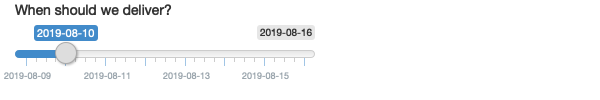
\includegraphics{images/date-slider.png}
\caption{placeholder}
\end{figure}

\begin{solution}
\leavevmode

\hypertarget{solution-6}{%
\subsubsection*{Solution}\label{solution-6}}
\addcontentsline{toc}{subsubsection}{Solution}

To create such slider, we need the following code.

\begin{Shaded}
\begin{Highlighting}[]
\FunctionTok{sliderInput}\NormalTok{(}
  \StringTok{"dates"}\NormalTok{,}
  \StringTok{"When should we deliver?"}\NormalTok{,}
  \AttributeTok{min =} \FunctionTok{as.Date}\NormalTok{(}\StringTok{"2019{-}08{-}09"}\NormalTok{),}
  \AttributeTok{max =} \FunctionTok{as.Date}\NormalTok{(}\StringTok{"2019{-}08{-}16"}\NormalTok{),}
  \AttributeTok{value =} \FunctionTok{as.Date}\NormalTok{(}\StringTok{"2019{-}08{-}10"}\NormalTok{)}
\NormalTok{)}
\end{Highlighting}
\end{Shaded}

\end{solution}

\hypertarget{exercise-3.2.8.3}{%
\subsection*{Exercise 3.2.8.3}\label{exercise-3.2.8.3}}
\addcontentsline{toc}{subsection}{Exercise 3.2.8.3}

If you have a moderately long list, it's useful to create sub-headings that
break the list up into pieces. Read the documentation for \texttt{selectInput()} to
figure out how. (Hint: the underlying HTML is called \texttt{\textless{}optgroup\textgreater{}}.)

\begin{solution}
\leavevmode

\hypertarget{solution-7}{%
\subsubsection*{Solution}\label{solution-7}}
\addcontentsline{toc}{subsubsection}{Solution}

We can make the \texttt{choices} argument a list of key-value pairs where the keys
represent the sub-headings and the values are lists containing the categorized
elements by keys. As an illustration, the following example separates animal breeds into two keys (categories): ``dogs'' and ``cats''.

\begin{Shaded}
\begin{Highlighting}[]
\FunctionTok{selectInput}\NormalTok{(}
  \StringTok{"breed"}\NormalTok{,}
  \StringTok{"Select your favorite animal breed:"}\NormalTok{,}
  \AttributeTok{choices =}
    \FunctionTok{list}\NormalTok{(}\StringTok{\textasciigrave{}}\AttributeTok{dogs}\StringTok{\textasciigrave{}} \OtherTok{=} \FunctionTok{list}\NormalTok{(}\StringTok{\textquotesingle{}German Shepherd\textquotesingle{}}\NormalTok{, }\StringTok{\textquotesingle{}Bulldog\textquotesingle{}}\NormalTok{, }\StringTok{\textquotesingle{}Labrador Retriever\textquotesingle{}}\NormalTok{),}
         \StringTok{\textasciigrave{}}\AttributeTok{cats}\StringTok{\textasciigrave{}} \OtherTok{=} \FunctionTok{list}\NormalTok{(}\StringTok{\textquotesingle{}Persian cat\textquotesingle{}}\NormalTok{, }\StringTok{\textquotesingle{}Bengal cat\textquotesingle{}}\NormalTok{, }\StringTok{\textquotesingle{}Siamese Cat\textquotesingle{}}\NormalTok{))}
\NormalTok{)}
\end{Highlighting}
\end{Shaded}

If you run the snippet above in the console, you will see the HTML code needed
to generate the input. You can also see the \texttt{\textless{}optgroup\textgreater{}} as hinted in the
exercise.

\end{solution}

\hypertarget{exercise-3.2.8.4}{%
\subsection*{Exercise 3.2.8.4}\label{exercise-3.2.8.4}}
\addcontentsline{toc}{subsection}{Exercise 3.2.8.4}

Create a slider input to select values between 0 and 100 where the interval
between each selectable value on the slider is 5. Then, add animation to the
input widget so when the user presses play the input widget scrolls through
automatically.

\begin{solution}
\leavevmode

\hypertarget{solution-8}{%
\subsubsection*{Solution}\label{solution-8}}
\addcontentsline{toc}{subsubsection}{Solution}

We can set the interval between each selectable value using the \texttt{step}
argument. In addition, by setting \texttt{animate\ =\ TRUE}, the slider will
automatically animate once the user presses play.

\begin{Shaded}
\begin{Highlighting}[]
  \FunctionTok{sliderInput}\NormalTok{(}\StringTok{"number"}\NormalTok{, }\StringTok{"Select a number:"}\NormalTok{,}
              \AttributeTok{min =} \DecValTok{0}\NormalTok{, }\AttributeTok{max =} \DecValTok{100}\NormalTok{, }\AttributeTok{value =} \DecValTok{0}\NormalTok{, }
              \AttributeTok{step =} \DecValTok{5}\NormalTok{, }\AttributeTok{animate =} \ConstantTok{TRUE}\NormalTok{)}
\end{Highlighting}
\end{Shaded}

\end{solution}

\hypertarget{exercise-3.2.8.5}{%
\subsection*{Exercise 3.2.8.5}\label{exercise-3.2.8.5}}
\addcontentsline{toc}{subsection}{Exercise 3.2.8.5}

Using the following numeric input box the user can enter any value between 0
and 1000. What is the purpose of the step argument in this widget?

\begin{Shaded}
\begin{Highlighting}[]
\FunctionTok{numericInput}\NormalTok{(}\StringTok{"number"}\NormalTok{, }\StringTok{"Select a value"}\NormalTok{, }\AttributeTok{value =} \DecValTok{150}\NormalTok{, }\AttributeTok{min =} \DecValTok{0}\NormalTok{, }\AttributeTok{max =} \DecValTok{1000}\NormalTok{, }\AttributeTok{step =} \DecValTok{50}\NormalTok{)}
\end{Highlighting}
\end{Shaded}

\begin{solution}
\leavevmode

\hypertarget{solution-9}{%
\subsubsection*{Solution}\label{solution-9}}
\addcontentsline{toc}{subsubsection}{Solution}

The step argument is the amount by which the \texttt{numericInput} value is
incremented (resp. decreased) when the user clicks the up (resp. down) arrow.
In the previous example, when the user clicks the up (resp. down) arrow the
numeric value will increase (resp. decrease) by 50. Note: by using a
\texttt{numericInput} the user still has the ability to type \emph{any} number.

\end{solution}

\hypertarget{exercise-3.3.5.1}{%
\subsection*{Exercise 3.3.5.1}\label{exercise-3.3.5.1}}
\addcontentsline{toc}{subsection}{Exercise 3.3.5.1}

Re-create the Shiny app from the plots section, this time setting height to
300px and width to 700px.

\begin{solution}
\leavevmode

\hypertarget{solution-10}{%
\subsubsection*{Solution}\label{solution-10}}
\addcontentsline{toc}{subsubsection}{Solution}

The function \texttt{plotOutput} can take on static \texttt{width} and \texttt{height} arguments.
Using the app from the plots section, we only need to add the height argument
and modify the width.

\begin{Shaded}
\begin{Highlighting}[]
\FunctionTok{library}\NormalTok{(shiny)}

\NormalTok{ui }\OtherTok{\textless{}{-}} \FunctionTok{fluidPage}\NormalTok{(}
  \FunctionTok{plotOutput}\NormalTok{(}\StringTok{"plot"}\NormalTok{, }\AttributeTok{width =} \StringTok{"700px"}\NormalTok{, }\AttributeTok{height =} \StringTok{"300px"}\NormalTok{)}
\NormalTok{)}

\NormalTok{server }\OtherTok{\textless{}{-}} \ControlFlowTok{function}\NormalTok{(input, output, session) \{}
\NormalTok{  output}\SpecialCharTok{$}\NormalTok{plot }\OtherTok{\textless{}{-}} \FunctionTok{renderPlot}\NormalTok{(}\FunctionTok{plot}\NormalTok{(}\DecValTok{1}\SpecialCharTok{:}\DecValTok{5}\NormalTok{), }\AttributeTok{res =} \DecValTok{96}\NormalTok{)}
\NormalTok{\}}

\FunctionTok{shinyApp}\NormalTok{(ui, server)}
\end{Highlighting}
\end{Shaded}

\end{solution}

\hypertarget{exercise-3.3.5.2}{%
\subsection*{Exercise 3.3.5.2}\label{exercise-3.3.5.2}}
\addcontentsline{toc}{subsection}{Exercise 3.3.5.2}

Update the options for renderDataTable() below so that the table is displayed, but nothing else (i.e.~remove the search, ordering, and filtering commands). You'll need to read ?renderDataTable and review the options at \url{https://datatables.net/reference/option/}.

\begin{Shaded}
\begin{Highlighting}[]
\NormalTok{ui }\OtherTok{\textless{}{-}} \FunctionTok{fluidPage}\NormalTok{(}
  \FunctionTok{dataTableOutput}\NormalTok{(}\StringTok{"table"}\NormalTok{)}
\NormalTok{)}
\NormalTok{server }\OtherTok{\textless{}{-}} \ControlFlowTok{function}\NormalTok{(input, output, session) \{}
\NormalTok{  output}\SpecialCharTok{$}\NormalTok{table }\OtherTok{\textless{}{-}} \FunctionTok{renderDataTable}\NormalTok{(mtcars, }\AttributeTok{options =} \FunctionTok{list}\NormalTok{(}\AttributeTok{pageLength =} \DecValTok{5}\NormalTok{))}
\NormalTok{\}}
\end{Highlighting}
\end{Shaded}

\begin{solution}
\leavevmode

\hypertarget{solution-11}{%
\subsubsection*{Solution}\label{solution-11}}
\addcontentsline{toc}{subsubsection}{Solution}

We can achieve this by setting \texttt{ordering} and \texttt{searching} to \texttt{FALSE} within the
\texttt{options} list.

\begin{Shaded}
\begin{Highlighting}[]
\FunctionTok{library}\NormalTok{(shiny)}

\NormalTok{ui }\OtherTok{\textless{}{-}} \FunctionTok{fluidPage}\NormalTok{(}
  \FunctionTok{dataTableOutput}\NormalTok{(}\StringTok{"table"}\NormalTok{)}
\NormalTok{)}

\NormalTok{server }\OtherTok{\textless{}{-}} \ControlFlowTok{function}\NormalTok{(input, output, session) \{}
\NormalTok{  output}\SpecialCharTok{$}\NormalTok{table }\OtherTok{\textless{}{-}} \FunctionTok{renderDataTable}\NormalTok{(}
\NormalTok{    mtcars, }\AttributeTok{options =} \FunctionTok{list}\NormalTok{(}\AttributeTok{ordering =} \ConstantTok{FALSE}\NormalTok{, }\AttributeTok{searching =} \ConstantTok{FALSE}\NormalTok{))}
\NormalTok{\}}

\FunctionTok{shinyApp}\NormalTok{(ui, server)}
\end{Highlighting}
\end{Shaded}

\end{solution}

\hypertarget{exercise-3.4.6.1}{%
\subsection*{Exercise 3.4.6.1}\label{exercise-3.4.6.1}}
\addcontentsline{toc}{subsection}{Exercise 3.4.6.1}

Create an app that contains two plots, each of which takes up half the app (regardless of what size the whole app is)

\begin{solution}
\leavevmode

\hypertarget{solution-12}{%
\subsubsection*{Solution}\label{solution-12}}
\addcontentsline{toc}{subsubsection}{Solution}

When creating the layout of a shiny app, you can use the \texttt{fluidRow} function to
control the width of the objects it contains. This function can have columns
and such columns can be set to have widths ranging from 1-12. Note that columns
width within a \texttt{fluidRow} container should add up to 12.

For our exercise, we need two columns of 50\% width each, i.e., we should set
the width of each column to 6.

\begin{Shaded}
\begin{Highlighting}[]
\FunctionTok{library}\NormalTok{(shiny)}

\NormalTok{ui }\OtherTok{\textless{}{-}} \FunctionTok{fluidPage}\NormalTok{(}
  \FunctionTok{fluidRow}\NormalTok{(}
    \FunctionTok{column}\NormalTok{(}\AttributeTok{width =} \DecValTok{6}\NormalTok{, }\FunctionTok{plotOutput}\NormalTok{(}\StringTok{"plot1"}\NormalTok{)),}
    \FunctionTok{column}\NormalTok{(}\AttributeTok{width =} \DecValTok{6}\NormalTok{, }\FunctionTok{plotOutput}\NormalTok{(}\StringTok{"plot2"}\NormalTok{))}
\NormalTok{  )}
\NormalTok{)}
\NormalTok{server }\OtherTok{\textless{}{-}} \ControlFlowTok{function}\NormalTok{(input, output, session) \{}
\NormalTok{  output}\SpecialCharTok{$}\NormalTok{plot1 }\OtherTok{\textless{}{-}} \FunctionTok{renderPlot}\NormalTok{(}\FunctionTok{plot}\NormalTok{(}\DecValTok{1}\SpecialCharTok{:}\DecValTok{5}\NormalTok{))}
\NormalTok{  output}\SpecialCharTok{$}\NormalTok{plot2 }\OtherTok{\textless{}{-}} \FunctionTok{renderPlot}\NormalTok{(}\FunctionTok{plot}\NormalTok{(}\DecValTok{1}\SpecialCharTok{:}\DecValTok{5}\NormalTok{))}
\NormalTok{\}}

\FunctionTok{shinyApp}\NormalTok{(ui, server)}
\end{Highlighting}
\end{Shaded}

\end{solution}

\hypertarget{exercise-3.4.6.2}{%
\subsection*{Exercise 3.4.6.2}\label{exercise-3.4.6.2}}
\addcontentsline{toc}{subsection}{Exercise 3.4.6.2}

Modify the Central Limit Theorem app so that the sidebar is on the right
instead of the left.

\begin{solution}
\leavevmode

\hypertarget{solution-13}{%
\subsubsection*{Solution}\label{solution-13}}
\addcontentsline{toc}{subsubsection}{Solution}

Looking at \texttt{?sidebarLayout} we can simply set the \texttt{position} argument to
\texttt{right}. We only need to modify the UI of the app.

\begin{Shaded}
\begin{Highlighting}[]
\NormalTok{ui }\OtherTok{\textless{}{-}} \FunctionTok{fluidPage}\NormalTok{(}
  \FunctionTok{headerPanel}\NormalTok{(}\StringTok{"Central limit theorem"}\NormalTok{),}
  \FunctionTok{sidebarLayout}\NormalTok{(}
    \AttributeTok{position =} \StringTok{"right"}\NormalTok{,}
    \FunctionTok{sidebarPanel}\NormalTok{(}
      \FunctionTok{numericInput}\NormalTok{(}\StringTok{"m"}\NormalTok{, }\StringTok{"Number of samples:"}\NormalTok{, }\DecValTok{2}\NormalTok{, }\AttributeTok{min =} \DecValTok{1}\NormalTok{, }\AttributeTok{max =} \DecValTok{100}\NormalTok{)}
\NormalTok{    ),}
    \FunctionTok{mainPanel}\NormalTok{(}
      \FunctionTok{plotOutput}\NormalTok{(}\StringTok{"hist"}\NormalTok{)}
\NormalTok{    )}
\NormalTok{  )}
\NormalTok{)}
\end{Highlighting}
\end{Shaded}

\end{solution}

\hypertarget{exercise-3.4.6.3}{%
\subsection*{Exercise 3.4.6.3}\label{exercise-3.4.6.3}}
\addcontentsline{toc}{subsection}{Exercise 3.4.6.3}

Browse the themes available in the shinythemes package, pick an attractive
theme, and apply it to the Central Limit Theorem app.

\begin{solution}
\leavevmode

\hypertarget{solution-14}{%
\subsubsection*{Solution}\label{solution-14}}
\addcontentsline{toc}{subsubsection}{Solution}

We can browse the themes \href{https://rstudio.github.io/shinythemes/}{here} and
apply it by setting the \texttt{theme} argument within \texttt{fluidPage} to
\texttt{shinythemes::shinytheme("theme\_name")}

\begin{Shaded}
\begin{Highlighting}[]
\FunctionTok{library}\NormalTok{(shinythemes)}

\NormalTok{ui }\OtherTok{\textless{}{-}} \FunctionTok{fluidPage}\NormalTok{(}
  \AttributeTok{theme =}\NormalTok{ shinythemes}\SpecialCharTok{::}\FunctionTok{shinytheme}\NormalTok{(}\StringTok{"darkly"}\NormalTok{),}
  \FunctionTok{headerPanel}\NormalTok{(}\StringTok{"Central limit theorem"}\NormalTok{),}
  \FunctionTok{sidebarLayout}\NormalTok{(}
    \AttributeTok{position =} \StringTok{"right"}\NormalTok{,}
    \FunctionTok{sidebarPanel}\NormalTok{(}
      \FunctionTok{numericInput}\NormalTok{(}\StringTok{"m"}\NormalTok{, }\StringTok{"Number of samples:"}\NormalTok{, }\DecValTok{2}\NormalTok{, }\AttributeTok{min =} \DecValTok{1}\NormalTok{, }\AttributeTok{max =} \DecValTok{100}\NormalTok{)}
\NormalTok{    ),}
    \FunctionTok{mainPanel}\NormalTok{(}
      \FunctionTok{plotOutput}\NormalTok{(}\StringTok{"hist"}\NormalTok{)}
\NormalTok{    )}
\NormalTok{  )}
\NormalTok{)}

\NormalTok{server }\OtherTok{\textless{}{-}} \ControlFlowTok{function}\NormalTok{(input, output, session) \{}
\NormalTok{  output}\SpecialCharTok{$}\NormalTok{hist }\OtherTok{\textless{}{-}} \FunctionTok{renderPlot}\NormalTok{(\{}
\NormalTok{    means }\OtherTok{\textless{}{-}} \FunctionTok{replicate}\NormalTok{(}\FloatTok{1e4}\NormalTok{, }\FunctionTok{mean}\NormalTok{(}\FunctionTok{runif}\NormalTok{(input}\SpecialCharTok{$}\NormalTok{m)))}
    \FunctionTok{hist}\NormalTok{(means, }\AttributeTok{breaks =} \DecValTok{20}\NormalTok{)}
\NormalTok{  \})}
\NormalTok{\}}

\FunctionTok{shinyApp}\NormalTok{(ui, server)}
\end{Highlighting}
\end{Shaded}

\end{solution}

\hypertarget{basic-reactivity}{%
\chapter{Basic Reactivity}\label{basic-reactivity}}

\hypertarget{exercise-4.3.6.1}{%
\subsection*{Exercise 4.3.6.1}\label{exercise-4.3.6.1}}
\addcontentsline{toc}{subsection}{Exercise 4.3.6.1}

Draw the reactive graph for the following server functions:

\begin{Shaded}
\begin{Highlighting}[]
\NormalTok{server1 }\OtherTok{\textless{}{-}} \ControlFlowTok{function}\NormalTok{(input, output, session) \{}
\NormalTok{  c }\OtherTok{\textless{}{-}} \FunctionTok{reactive}\NormalTok{(input}\SpecialCharTok{$}\NormalTok{a }\SpecialCharTok{+}\NormalTok{ input}\SpecialCharTok{$}\NormalTok{b)}
\NormalTok{  e }\OtherTok{\textless{}{-}} \FunctionTok{reactive}\NormalTok{(}\FunctionTok{c}\NormalTok{() }\SpecialCharTok{+}\NormalTok{ input}\SpecialCharTok{$}\NormalTok{d)}
\NormalTok{  output}\SpecialCharTok{$}\NormalTok{f }\OtherTok{\textless{}{-}} \FunctionTok{renderText}\NormalTok{(}\FunctionTok{e}\NormalTok{())}
\NormalTok{\}}

\NormalTok{server2 }\OtherTok{\textless{}{-}} \ControlFlowTok{function}\NormalTok{(input, output, session) \{}
\NormalTok{  x }\OtherTok{\textless{}{-}} \FunctionTok{reactive}\NormalTok{(input}\SpecialCharTok{$}\NormalTok{x1 }\SpecialCharTok{+}\NormalTok{ input}\SpecialCharTok{$}\NormalTok{x2 }\SpecialCharTok{+}\NormalTok{ input}\SpecialCharTok{$}\NormalTok{x3)}
\NormalTok{  y }\OtherTok{\textless{}{-}} \FunctionTok{reactive}\NormalTok{(input}\SpecialCharTok{$}\NormalTok{y1 }\SpecialCharTok{+}\NormalTok{ input}\SpecialCharTok{$}\NormalTok{y2)}
\NormalTok{  output}\SpecialCharTok{$}\NormalTok{z }\OtherTok{\textless{}{-}} \FunctionTok{renderText}\NormalTok{(}\FunctionTok{x}\NormalTok{() }\SpecialCharTok{/} \FunctionTok{y}\NormalTok{())}
\NormalTok{\}}

\NormalTok{server3 }\OtherTok{\textless{}{-}} \ControlFlowTok{function}\NormalTok{(input, output, session) \{}
\NormalTok{  d }\OtherTok{\textless{}{-}} \FunctionTok{reactive}\NormalTok{(}\FunctionTok{c}\NormalTok{() }\SpecialCharTok{\^{}}\NormalTok{ input}\SpecialCharTok{$}\NormalTok{d)}
\NormalTok{  a }\OtherTok{\textless{}{-}} \FunctionTok{reactive}\NormalTok{(input}\SpecialCharTok{$}\NormalTok{a }\SpecialCharTok{*} \DecValTok{10}\NormalTok{)}
\NormalTok{  c }\OtherTok{\textless{}{-}} \FunctionTok{reactive}\NormalTok{(}\FunctionTok{b}\NormalTok{() }\SpecialCharTok{/}\NormalTok{ input}\SpecialCharTok{$}\NormalTok{c)}
\NormalTok{  b }\OtherTok{\textless{}{-}} \FunctionTok{reactive}\NormalTok{(}\FunctionTok{a}\NormalTok{() }\SpecialCharTok{+}\NormalTok{ input}\SpecialCharTok{$}\NormalTok{b)}
\NormalTok{\}}
\end{Highlighting}
\end{Shaded}

\begin{solution}
\leavevmode

\hypertarget{solution-15}{%
\subsubsection*{Solution}\label{solution-15}}
\addcontentsline{toc}{subsubsection}{Solution}

To create the reactive graph we need to consider the inputs, reactive
expressions, and outputs of the app.

For \texttt{server1} we have the following objects:

\begin{itemize}
\tightlist
\item
  inputs: \texttt{input\$a}, \texttt{input\$b}, and \texttt{input\$d}
\item
  reactives: \texttt{c()} and \texttt{e()}
\item
  outputs: \texttt{output\$f}
\end{itemize}

Inputs \texttt{input\$a} and \texttt{input\$b} are used to create \texttt{c()}, which is combined with
\texttt{input\$d} to create \texttt{e()}. The output depends only on \texttt{e()}.

\begin{figure}
\centering
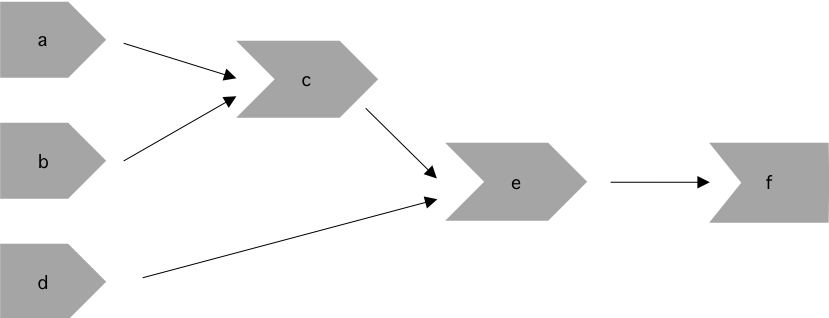
\includegraphics[width=5.20833in,height=\textheight]{images/4.3.6.1-s1.png}
\caption{reactive graph - server 1}
\end{figure}

For \texttt{server2} we have the following objects:

\begin{itemize}
\tightlist
\item
  inputs: \texttt{input\$y1}, \texttt{input\$y2}, \texttt{input\$x1}, \texttt{input\$x2}, \texttt{input\$x3}
\item
  reactives: \texttt{y()} and \texttt{x()}
\item
  outputs: \texttt{output\$z}
\end{itemize}

Inputs \texttt{input\$y1} and \texttt{input\$y2} are needed to create the reactive \texttt{y()}. In
addition, inputs \texttt{input\$x1}, \texttt{input\$x2}, and \texttt{input\$x3} are required to create
the reactive \texttt{x()}. The output depends on both \texttt{x()} and \texttt{y()}.

\begin{figure}
\centering
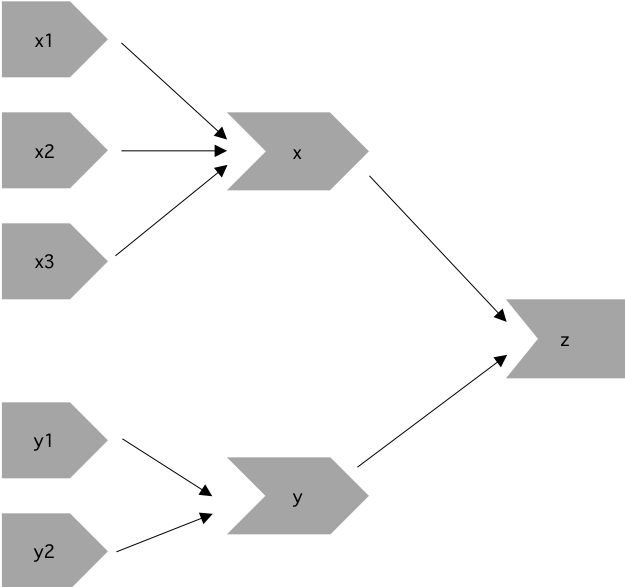
\includegraphics[width=4.16667in,height=\textheight]{images/4.3.6.1-s2.png}
\caption{reactive graph - server 2}
\end{figure}

For \texttt{server3} we have the following objects:

\begin{itemize}
\tightlist
\item
  inputs: \texttt{input\$a}, \texttt{input\$b}, \texttt{input\$c}, \texttt{input\$d}
\item
  reactives: \texttt{a()}, \texttt{b()}, \texttt{c()}, \texttt{d()}
\end{itemize}

As we can see below, \texttt{a()} relies on \texttt{input\$a}, \texttt{b()} relies on both \texttt{a()} and
\texttt{input\$b}, and \texttt{c()} relies on both \texttt{b()} and \texttt{input\$c}. The final output
depends on both \texttt{c()} and \texttt{input\$d}.

\begin{figure}
\centering
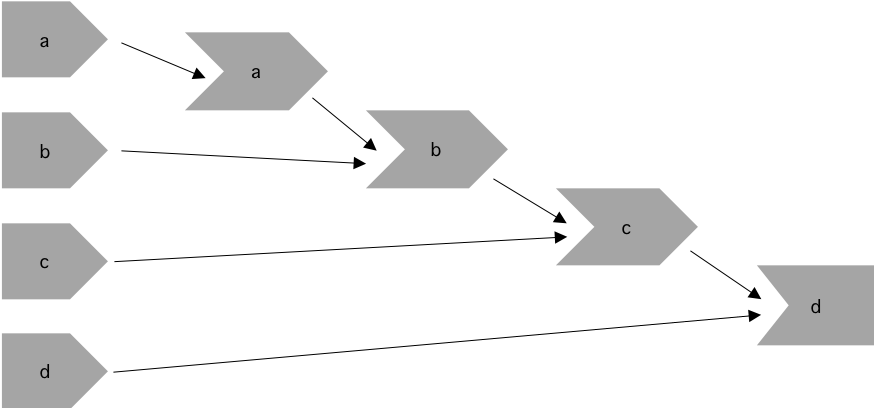
\includegraphics[width=6.25in,height=\textheight]{images/4.3.6.1-s3.png}
\caption{reactive graph - server 3}
\end{figure}

\end{solution}

\hypertarget{exercise-4.3.6.2}{%
\subsection*{Exercise 4.3.6.2}\label{exercise-4.3.6.2}}
\addcontentsline{toc}{subsection}{Exercise 4.3.6.2}

Why will this code fail?

\begin{Shaded}
\begin{Highlighting}[]
\NormalTok{var }\OtherTok{\textless{}{-}} \FunctionTok{reactive}\NormalTok{(df[input}\SpecialCharTok{$}\NormalTok{var])}
\NormalTok{range }\OtherTok{\textless{}{-}} \FunctionTok{reactive}\NormalTok{(}\FunctionTok{range}\NormalTok{(}\FunctionTok{var}\NormalTok{(), }\AttributeTok{na.rm =} \ConstantTok{TRUE}\NormalTok{))}
\end{Highlighting}
\end{Shaded}

Why is \texttt{var()} a bad name for a reactive?

\begin{solution}
\leavevmode

\hypertarget{solution-16}{%
\subsubsection*{Solution}\label{solution-16}}
\addcontentsline{toc}{subsubsection}{Solution}

This code doesn't work because we called our reactive \texttt{range}, so when we call the \texttt{range} function we're actually calling our new reactive. If we change the name of the reactive from \texttt{range} to \texttt{col\_range} then the code will work. Similarly, \texttt{var()} is not a good name for a reactive because it's already a function to compute the variance of \texttt{x}! \texttt{?cor::var}

\begin{Shaded}
\begin{Highlighting}[]
\FunctionTok{library}\NormalTok{(shiny)}

\NormalTok{df }\OtherTok{\textless{}{-}}\NormalTok{ mtcars}

\NormalTok{ui }\OtherTok{\textless{}{-}} \FunctionTok{fluidPage}\NormalTok{(}
    \FunctionTok{selectInput}\NormalTok{(}\StringTok{"var"}\NormalTok{, }\ConstantTok{NULL}\NormalTok{, }\AttributeTok{choices =} \FunctionTok{colnames}\NormalTok{(df)),}
    \FunctionTok{verbatimTextOutput}\NormalTok{(}\StringTok{"debug"}\NormalTok{)}
\NormalTok{)}

\NormalTok{server }\OtherTok{\textless{}{-}} \ControlFlowTok{function}\NormalTok{(input, output, session) \{}
\NormalTok{    col\_var }\OtherTok{\textless{}{-}} \FunctionTok{reactive}\NormalTok{( df[input}\SpecialCharTok{$}\NormalTok{var] )}
\NormalTok{    col\_range }\OtherTok{\textless{}{-}} \FunctionTok{reactive}\NormalTok{(\{ }\FunctionTok{range}\NormalTok{(}\FunctionTok{col\_var}\NormalTok{(), }\AttributeTok{na.rm =} \ConstantTok{TRUE}\NormalTok{ ) \})}
\NormalTok{    output}\SpecialCharTok{$}\NormalTok{debug }\OtherTok{\textless{}{-}} \FunctionTok{renderPrint}\NormalTok{(\{ }\FunctionTok{col\_range}\NormalTok{() \})}

\NormalTok{\}}

\FunctionTok{shinyApp}\NormalTok{(}\AttributeTok{ui =}\NormalTok{ ui, }\AttributeTok{server =}\NormalTok{ server)}
\end{Highlighting}
\end{Shaded}

\end{solution}

\hypertarget{exercise-4.4.6.1}{%
\subsection*{Exercise 4.4.6.1}\label{exercise-4.4.6.1}}
\addcontentsline{toc}{subsection}{Exercise 4.4.6.1}

Use reactive expressions to reduce the duplicated code in the following simple
apps.

\begin{solution}
\leavevmode

\hypertarget{solution-17}{%
\subsubsection*{Solution}\label{solution-17}}
\addcontentsline{toc}{subsubsection}{Solution}

Unclear about the apps mentioned in the exercise.

\end{solution}

\hypertarget{case-study-er-injuries}{%
\chapter{Case Study: ER Injuries}\label{case-study-er-injuries}}

\hypertarget{exercise-5.8.1}{%
\subsection*{Exercise 5.8.1}\label{exercise-5.8.1}}
\addcontentsline{toc}{subsection}{Exercise 5.8.1}

Draw the reactive graph for each app.

\begin{solution}
\leavevmode

\hypertarget{solution-18}{%
\subsubsection*{Solution}\label{solution-18}}
\addcontentsline{toc}{subsubsection}{Solution}

\hypertarget{prototype}{%
\paragraph*{Prototype}\label{prototype}}
\addcontentsline{toc}{paragraph}{Prototype}

The prototype application has a single input, \texttt{input\$code}, which is used to
generate the \texttt{selected()} reactive. This reactive is used directly in 3
outputs, \texttt{output\$diag}, \texttt{output\$body\_part}, and \texttt{output\$location}, and it is
also used indirectly in the \texttt{output\$age\_sex} plot via the \texttt{summary()} reactive.

\begin{figure}
\centering
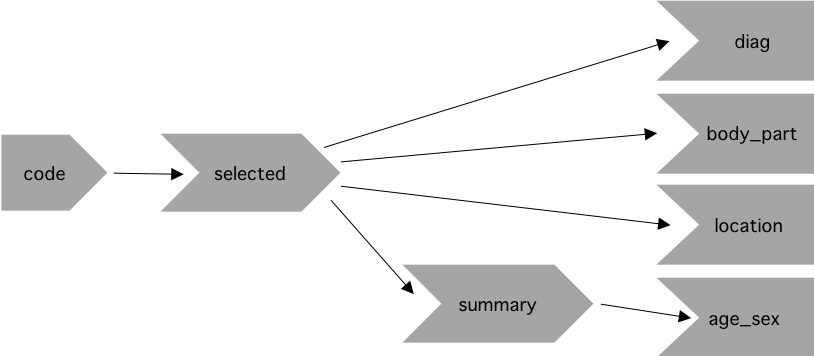
\includegraphics[width=5.20833in,height=\textheight]{images/5.8.1-prototype.png}
\caption{reactive graph - prototype app}
\end{figure}

\hypertarget{rate-vs.-count}{%
\paragraph*{Rate vs.~Count}\label{rate-vs.-count}}
\addcontentsline{toc}{paragraph}{Rate vs.~Count}

Building on the prototype, we create a second input \texttt{input\$y} which is used
along with the \texttt{summary()} reactive to create the \texttt{output\$age\_sex} plot.

\begin{figure}
\centering
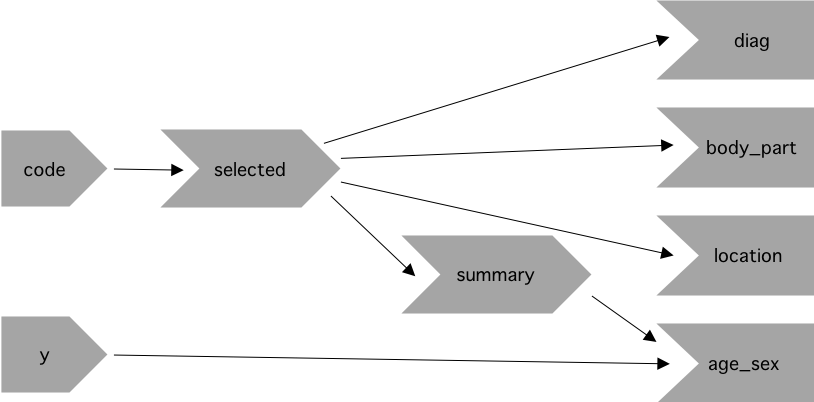
\includegraphics[width=5.20833in,height=\textheight]{images/5.8.1-ratecount.png}
\caption{reactive graph - rate vs.~count app}
\end{figure}

\hypertarget{narrative}{%
\paragraph*{Narrative}\label{narrative}}
\addcontentsline{toc}{paragraph}{Narrative}

Building on the application once more, we create an \texttt{output\$narrative} that
depends on the \texttt{selected()} reactive and a new input, \texttt{input\$story}.

\begin{figure}
\centering
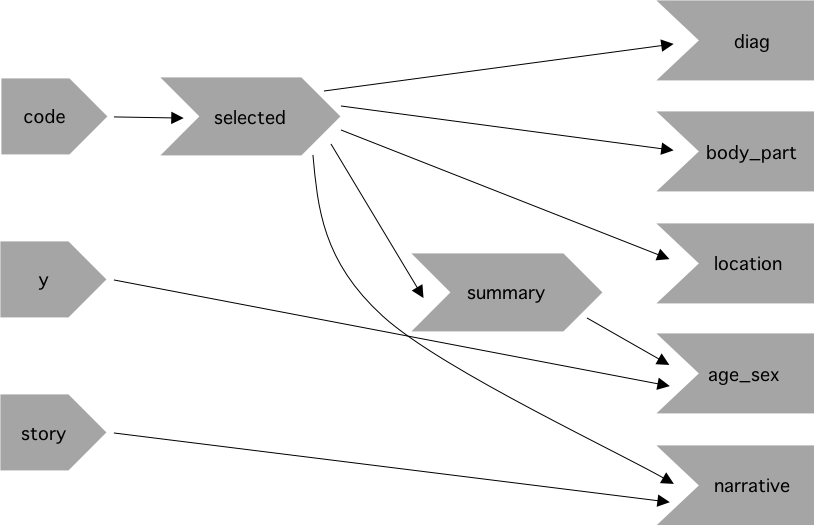
\includegraphics[width=5.20833in,height=\textheight]{images/5.8.1-narrative.png}
\caption{reactive graph - narrative app}
\end{figure}

\end{solution}

\hypertarget{exercise-5.8.2}{%
\subsection*{Exercise 5.8.2}\label{exercise-5.8.2}}
\addcontentsline{toc}{subsection}{Exercise 5.8.2}

What happens if you flip \texttt{fct\_infreq()} and \texttt{fct\_lump()} in the code that
reduces the summary tables?

\begin{solution}
\leavevmode

\hypertarget{solution-19}{%
\subsubsection*{Solution}\label{solution-19}}
\addcontentsline{toc}{subsubsection}{Solution}

As in the book, we will use the datasets \texttt{injuries}, \texttt{products}, and
\texttt{population} appearing here:
\url{https://github.com/hadley/mastering-shiny/blob/main/neiss/data.R}.

Flipping the order of \texttt{fct\_infreq()} and \texttt{fct\_lump()} will only change the
factor levels order. In particular, the function \texttt{fct\_infreq()} orders the
factor levels by frequency, and the function \texttt{fct\_lump()} also orders the
factor levels by frequency but it will only keep the top \texttt{n} factors and label
the rest as \texttt{Other}.

Let us look at the top five levels in terms of count within the \texttt{diag} column
in the \texttt{injuries} dataset:

\begin{Shaded}
\begin{Highlighting}[]
\NormalTok{injuries }\SpecialCharTok{\%\textgreater{}\%}
  \FunctionTok{group\_by}\NormalTok{(diag) }\SpecialCharTok{\%\textgreater{}\%}
  \FunctionTok{count}\NormalTok{() }\SpecialCharTok{\%\textgreater{}\%}
  \FunctionTok{arrange}\NormalTok{(}\SpecialCharTok{{-}}\NormalTok{n) }\SpecialCharTok{\%\textgreater{}\%}
  \FunctionTok{head}\NormalTok{(}\DecValTok{5}\NormalTok{)}
\end{Highlighting}
\end{Shaded}

\begin{verbatim}
## # A tibble: 5 x 2
## # Groups:   diag [5]
##   diag                      n
##   <chr>                 <int>
## 1 Other Or Not Stated   44937
## 2 Fracture              43093
## 3 Laceration            39230
## 4 Strain, Sprain        37002
## 5 Contusion Or Abrasion 35259
\end{verbatim}

If we apply \texttt{fct\_infreq()} first, then it will reorder the factor levels in
descending order as seen in the previous output. If afterwards we apply
\texttt{fct\_lump()}, then it will lump together everything after the nth most commonly
seen level.

\begin{Shaded}
\begin{Highlighting}[]
\NormalTok{diag }\OtherTok{\textless{}{-}}\NormalTok{ injuries }\SpecialCharTok{\%\textgreater{}\%}
  \FunctionTok{mutate}\NormalTok{(}\AttributeTok{diag =} \FunctionTok{fct\_lump}\NormalTok{(}\FunctionTok{fct\_infreq}\NormalTok{(diag), }\AttributeTok{n =} \DecValTok{5}\NormalTok{)) }\SpecialCharTok{\%\textgreater{}\%}
  \FunctionTok{pull}\NormalTok{(diag)}

\FunctionTok{levels}\NormalTok{(diag)}
\end{Highlighting}
\end{Shaded}

\begin{verbatim}
## [1] "Other Or Not Stated"   "Fracture"              "Laceration"           
## [4] "Strain, Sprain"        "Contusion Or Abrasion" "Other"
\end{verbatim}

Conversely, if we apply \texttt{fct\_lump()} first, then it will label the most
frequently seen factor level as ``Other''. If afterwards we apply \texttt{fct\_infreq()},
then it will label the first level as ``Other'' and not as ``Other Or Not Stated'',
which was the case for the previous code.

\begin{Shaded}
\begin{Highlighting}[]
\NormalTok{diag }\OtherTok{\textless{}{-}}\NormalTok{ injuries }\SpecialCharTok{\%\textgreater{}\%}
  \FunctionTok{mutate}\NormalTok{(}\AttributeTok{diag =} \FunctionTok{fct\_infreq}\NormalTok{(}\FunctionTok{fct\_lump}\NormalTok{(diag, }\AttributeTok{n =} \DecValTok{5}\NormalTok{))) }\SpecialCharTok{\%\textgreater{}\%}
  \FunctionTok{pull}\NormalTok{(diag)}

\FunctionTok{levels}\NormalTok{(diag)}
\end{Highlighting}
\end{Shaded}

\begin{verbatim}
## [1] "Other"                 "Other Or Not Stated"   "Fracture"             
## [4] "Laceration"            "Strain, Sprain"        "Contusion Or Abrasion"
\end{verbatim}

\end{solution}

\hypertarget{exercise-5.8.3}{%
\subsection*{Exercise 5.8.3}\label{exercise-5.8.3}}
\addcontentsline{toc}{subsection}{Exercise 5.8.3}

Add an input control that lets the user decide how many rows to show in the
summary tables.

\begin{solution}
\leavevmode

\hypertarget{solution-20}{%
\subsubsection*{Solution}\label{solution-20}}
\addcontentsline{toc}{subsubsection}{Solution}

Our function \texttt{count\_top} is responsible for grouping our variables into a set
number of factors, lumping the rest of the values into ``Other''. The function
has an argument \texttt{n} which is set to \texttt{5}. By creating a \texttt{numericInput} called
\texttt{rows} we can let the user set the number of \texttt{fct\_infreq} dynamically. However,
because \texttt{fct\_infreq} is the number of factors + \texttt{Other}, we need to subtract 1
from what the user selects in order to display the number of rows they input.

\begin{Shaded}
\begin{Highlighting}[]
\FunctionTok{library}\NormalTok{(shiny)}
\FunctionTok{library}\NormalTok{(forcats)}
\FunctionTok{library}\NormalTok{(dplyr)}
\FunctionTok{library}\NormalTok{(ggplot2)}

\CommentTok{\# Note: these exercises use the datasets \textasciigrave{}injuries\textasciigrave{}, \textasciigrave{}products\textasciigrave{}, and}
\CommentTok{\# \textasciigrave{}population\textasciigrave{} as created here:}
\CommentTok{\# https://github.com/hadley/mastering{-}shiny/blob/main/neiss/data.R}

\NormalTok{count\_top }\OtherTok{\textless{}{-}} \ControlFlowTok{function}\NormalTok{(df, var, }\AttributeTok{n =} \DecValTok{5}\NormalTok{) \{}
\NormalTok{  df }\SpecialCharTok{\%\textgreater{}\%}
    \FunctionTok{mutate}\NormalTok{(\{\{ var \}\} }\SpecialCharTok{:}\ErrorTok{=} \FunctionTok{fct\_lump}\NormalTok{(}\FunctionTok{fct\_infreq}\NormalTok{(\{\{ var \}\}), }\AttributeTok{n =}\NormalTok{ n)) }\SpecialCharTok{\%\textgreater{}\%}
    \FunctionTok{group\_by}\NormalTok{(\{\{ var \}\}) }\SpecialCharTok{\%\textgreater{}\%}
    \FunctionTok{summarise}\NormalTok{(}\AttributeTok{n =} \FunctionTok{as.integer}\NormalTok{(}\FunctionTok{sum}\NormalTok{(weight)))}
\NormalTok{\}}

\NormalTok{ui }\OtherTok{\textless{}{-}} \FunctionTok{fluidPage}\NormalTok{(}
  \FunctionTok{fluidRow}\NormalTok{(}
    \FunctionTok{column}\NormalTok{(}\DecValTok{8}\NormalTok{, }\FunctionTok{selectInput}\NormalTok{(}\StringTok{"code"}\NormalTok{, }\StringTok{"Product"}\NormalTok{,}
                          \AttributeTok{choices =} \FunctionTok{setNames}\NormalTok{(products}\SpecialCharTok{$}\NormalTok{prod\_code, products}\SpecialCharTok{$}\NormalTok{title),}
                          \AttributeTok{width =} \StringTok{"100\%"}\NormalTok{)}
\NormalTok{    ),}
    \FunctionTok{column}\NormalTok{(}\DecValTok{2}\NormalTok{, }\FunctionTok{numericInput}\NormalTok{(}\StringTok{"rows"}\NormalTok{, }\StringTok{"Number of Rows"}\NormalTok{,}
                           \AttributeTok{min =} \DecValTok{1}\NormalTok{, }\AttributeTok{max =} \DecValTok{10}\NormalTok{, }\AttributeTok{value =} \DecValTok{5}\NormalTok{)),}
    \FunctionTok{column}\NormalTok{(}\DecValTok{2}\NormalTok{, }\FunctionTok{selectInput}\NormalTok{(}\StringTok{"y"}\NormalTok{, }\StringTok{"Y Axis"}\NormalTok{, }\FunctionTok{c}\NormalTok{(}\StringTok{"rate"}\NormalTok{, }\StringTok{"count"}\NormalTok{)))}
\NormalTok{  ),}
  \FunctionTok{fluidRow}\NormalTok{(}
    \FunctionTok{column}\NormalTok{(}\DecValTok{4}\NormalTok{, }\FunctionTok{tableOutput}\NormalTok{(}\StringTok{"diag"}\NormalTok{)),}
    \FunctionTok{column}\NormalTok{(}\DecValTok{4}\NormalTok{, }\FunctionTok{tableOutput}\NormalTok{(}\StringTok{"body\_part"}\NormalTok{)),}
    \FunctionTok{column}\NormalTok{(}\DecValTok{4}\NormalTok{, }\FunctionTok{tableOutput}\NormalTok{(}\StringTok{"location"}\NormalTok{))}
\NormalTok{  ),}
  \FunctionTok{fluidRow}\NormalTok{(}
    \FunctionTok{column}\NormalTok{(}\DecValTok{12}\NormalTok{, }\FunctionTok{plotOutput}\NormalTok{(}\StringTok{"age\_sex"}\NormalTok{))}
\NormalTok{  ),}
  \FunctionTok{fluidRow}\NormalTok{(}
    \FunctionTok{column}\NormalTok{(}\DecValTok{2}\NormalTok{, }\FunctionTok{actionButton}\NormalTok{(}\StringTok{"story"}\NormalTok{, }\StringTok{"Tell me a story"}\NormalTok{)),}
    \FunctionTok{column}\NormalTok{(}\DecValTok{10}\NormalTok{, }\FunctionTok{textOutput}\NormalTok{(}\StringTok{"narrative"}\NormalTok{))}
\NormalTok{  )}
\NormalTok{)}

\NormalTok{server }\OtherTok{\textless{}{-}} \ControlFlowTok{function}\NormalTok{(input, output, session) \{}
\NormalTok{  selected }\OtherTok{\textless{}{-}} \FunctionTok{reactive}\NormalTok{(injuries }\SpecialCharTok{\%\textgreater{}\%} \FunctionTok{filter}\NormalTok{(prod\_code }\SpecialCharTok{==}\NormalTok{ input}\SpecialCharTok{$}\NormalTok{code))}
  
  \CommentTok{\# Find the maximum possible of rows.}
\NormalTok{  max\_no\_rows }\OtherTok{\textless{}{-}} \FunctionTok{reactive}\NormalTok{(}
    \FunctionTok{max}\NormalTok{(}\FunctionTok{length}\NormalTok{(}\FunctionTok{unique}\NormalTok{(}\FunctionTok{selected}\NormalTok{()}\SpecialCharTok{$}\NormalTok{diag)),}
        \FunctionTok{length}\NormalTok{(}\FunctionTok{unique}\NormalTok{(}\FunctionTok{selected}\NormalTok{()}\SpecialCharTok{$}\NormalTok{body\_part)),}
        \FunctionTok{length}\NormalTok{(}\FunctionTok{unique}\NormalTok{(}\FunctionTok{selected}\NormalTok{()}\SpecialCharTok{$}\NormalTok{location)))}
\NormalTok{  )}
  
  \CommentTok{\# Update the maximum value for the numericInput based on max\_no\_rows().}
  \FunctionTok{observeEvent}\NormalTok{(input}\SpecialCharTok{$}\NormalTok{code, \{}
    \FunctionTok{updateNumericInput}\NormalTok{(session, }\StringTok{"rows"}\NormalTok{, }\AttributeTok{max =} \FunctionTok{max\_no\_rows}\NormalTok{())}
\NormalTok{  \})}
  
\NormalTok{  table\_rows }\OtherTok{\textless{}{-}} \FunctionTok{reactive}\NormalTok{(input}\SpecialCharTok{$}\NormalTok{rows }\SpecialCharTok{{-}} \DecValTok{1}\NormalTok{)}
  
\NormalTok{  output}\SpecialCharTok{$}\NormalTok{diag }\OtherTok{\textless{}{-}} \FunctionTok{renderTable}\NormalTok{(}
    \FunctionTok{count\_top}\NormalTok{(}\FunctionTok{selected}\NormalTok{(), diag, }\AttributeTok{n =} \FunctionTok{table\_rows}\NormalTok{()), }\AttributeTok{width =} \StringTok{"100\%"}\NormalTok{)}
  
\NormalTok{  output}\SpecialCharTok{$}\NormalTok{body\_part }\OtherTok{\textless{}{-}} \FunctionTok{renderTable}\NormalTok{(}
    \FunctionTok{count\_top}\NormalTok{(}\FunctionTok{selected}\NormalTok{(), body\_part, }\AttributeTok{n =} \FunctionTok{table\_rows}\NormalTok{()), }\AttributeTok{width =} \StringTok{"100\%"}\NormalTok{)}
  
\NormalTok{  output}\SpecialCharTok{$}\NormalTok{location }\OtherTok{\textless{}{-}} \FunctionTok{renderTable}\NormalTok{(}
    \FunctionTok{count\_top}\NormalTok{(}\FunctionTok{selected}\NormalTok{(), location, }\AttributeTok{n =} \FunctionTok{table\_rows}\NormalTok{()), }\AttributeTok{width =} \StringTok{"100\%"}\NormalTok{)}
  
\NormalTok{  summary }\OtherTok{\textless{}{-}} \FunctionTok{reactive}\NormalTok{(\{}
    \FunctionTok{selected}\NormalTok{() }\SpecialCharTok{\%\textgreater{}\%}
      \FunctionTok{count}\NormalTok{(age, sex, }\AttributeTok{wt =}\NormalTok{ weight) }\SpecialCharTok{\%\textgreater{}\%}
      \FunctionTok{left\_join}\NormalTok{(population, }\AttributeTok{by =} \FunctionTok{c}\NormalTok{(}\StringTok{"age"}\NormalTok{, }\StringTok{"sex"}\NormalTok{)) }\SpecialCharTok{\%\textgreater{}\%}
      \FunctionTok{mutate}\NormalTok{(}\AttributeTok{rate =}\NormalTok{ n }\SpecialCharTok{/}\NormalTok{ population }\SpecialCharTok{*} \FloatTok{1e4}\NormalTok{)}
\NormalTok{  \})}
  
\NormalTok{  output}\SpecialCharTok{$}\NormalTok{age\_sex }\OtherTok{\textless{}{-}} \FunctionTok{renderPlot}\NormalTok{(\{}
    \ControlFlowTok{if}\NormalTok{ (input}\SpecialCharTok{$}\NormalTok{y }\SpecialCharTok{==} \StringTok{"count"}\NormalTok{) \{}
      \FunctionTok{summary}\NormalTok{() }\SpecialCharTok{\%\textgreater{}\%}
        \FunctionTok{ggplot}\NormalTok{(}\FunctionTok{aes}\NormalTok{(age, n, }\AttributeTok{colour =}\NormalTok{ sex)) }\SpecialCharTok{+}
        \FunctionTok{geom\_line}\NormalTok{() }\SpecialCharTok{+}
        \FunctionTok{labs}\NormalTok{(}\AttributeTok{y =} \StringTok{"Estimated number of injuries"}\NormalTok{) }\SpecialCharTok{+}
        \FunctionTok{theme\_grey}\NormalTok{(}\DecValTok{15}\NormalTok{)}
\NormalTok{    \} }\ControlFlowTok{else}\NormalTok{ \{}
      \FunctionTok{summary}\NormalTok{() }\SpecialCharTok{\%\textgreater{}\%}
        \FunctionTok{ggplot}\NormalTok{(}\FunctionTok{aes}\NormalTok{(age, rate, }\AttributeTok{colour =}\NormalTok{ sex)) }\SpecialCharTok{+}
        \FunctionTok{geom\_line}\NormalTok{(}\AttributeTok{na.rm =} \ConstantTok{TRUE}\NormalTok{) }\SpecialCharTok{+}
        \FunctionTok{labs}\NormalTok{(}\AttributeTok{y =} \StringTok{"Injuries per 10,000 people"}\NormalTok{) }\SpecialCharTok{+}
        \FunctionTok{theme\_grey}\NormalTok{(}\DecValTok{15}\NormalTok{)}
\NormalTok{    \}}
\NormalTok{  \})}
  
\NormalTok{  output}\SpecialCharTok{$}\NormalTok{narrative }\OtherTok{\textless{}{-}} \FunctionTok{renderText}\NormalTok{(\{}
\NormalTok{    input}\SpecialCharTok{$}\NormalTok{story}
    \FunctionTok{selected}\NormalTok{() }\SpecialCharTok{\%\textgreater{}\%} \FunctionTok{pull}\NormalTok{(narrative) }\SpecialCharTok{\%\textgreater{}\%} \FunctionTok{sample}\NormalTok{(}\DecValTok{1}\NormalTok{)}
\NormalTok{  \})}
\NormalTok{\}}

\FunctionTok{shinyApp}\NormalTok{(ui, server)}
\end{Highlighting}
\end{Shaded}

\end{solution}

\hypertarget{exercise-5.8.4}{%
\subsection*{Exercise 5.8.4}\label{exercise-5.8.4}}
\addcontentsline{toc}{subsection}{Exercise 5.8.4}

Provide a way to step through every narrative systematically with forward and
backward buttons.

Advanced: Make the list of narratives ``circular'' so that advancing forward from
the last narrative takes you to the first.

\begin{solution}
\leavevmode

\hypertarget{solution-21}{%
\subsubsection*{Solution}\label{solution-21}}
\addcontentsline{toc}{subsubsection}{Solution}

We can add two action buttons \texttt{prev\_story} and \texttt{next\_story} to iterate through the
narrative. We can leverage the fact that whenever you click an action button in Shiny, the button stores how many times that button has been clicked. To caculate the index of the current story, we can subtract the stored count of the \texttt{next\_story} button from the \texttt{previous\_story} button. Then, by using the modulus operator, we can increase the current position in the narrative while never go beyond the interval {[}1, length of the narrative{]}.

\begin{Shaded}
\begin{Highlighting}[]
\FunctionTok{library}\NormalTok{(shiny)}
\FunctionTok{library}\NormalTok{(forcats)}
\FunctionTok{library}\NormalTok{(dplyr)}
\FunctionTok{library}\NormalTok{(ggplot2)}

\CommentTok{\# Note: these exercises use the datasets \textasciigrave{}injuries\textasciigrave{}, \textasciigrave{}products\textasciigrave{}, and}
\CommentTok{\# \textasciigrave{}population\textasciigrave{} as created here:}
\CommentTok{\# https://github.com/hadley/mastering{-}shiny/blob/main/neiss/data.R}

\NormalTok{count\_top }\OtherTok{\textless{}{-}} \ControlFlowTok{function}\NormalTok{(df, var, }\AttributeTok{n =} \DecValTok{5}\NormalTok{) \{}
\NormalTok{  df }\SpecialCharTok{\%\textgreater{}\%}
    \FunctionTok{mutate}\NormalTok{(\{\{ var \}\} }\SpecialCharTok{:}\ErrorTok{=} \FunctionTok{fct\_lump}\NormalTok{(}\FunctionTok{fct\_infreq}\NormalTok{(\{\{ var \}\}), }\AttributeTok{n =}\NormalTok{ n)) }\SpecialCharTok{\%\textgreater{}\%}
    \FunctionTok{group\_by}\NormalTok{(\{\{ var \}\}) }\SpecialCharTok{\%\textgreater{}\%}
    \FunctionTok{summarise}\NormalTok{(}\AttributeTok{n =} \FunctionTok{as.integer}\NormalTok{(}\FunctionTok{sum}\NormalTok{(weight)))}
\NormalTok{\}}

\NormalTok{ui }\OtherTok{\textless{}{-}} \FunctionTok{fluidPage}\NormalTok{(}
  \FunctionTok{fluidRow}\NormalTok{(}
    \FunctionTok{column}\NormalTok{(}\DecValTok{8}\NormalTok{, }\FunctionTok{selectInput}\NormalTok{(}\StringTok{"code"}\NormalTok{, }\StringTok{"Product"}\NormalTok{,}
                          \AttributeTok{choices =} \FunctionTok{setNames}\NormalTok{(products}\SpecialCharTok{$}\NormalTok{prod\_code, products}\SpecialCharTok{$}\NormalTok{title),}
                          \AttributeTok{width =} \StringTok{"100\%"}\NormalTok{)}
\NormalTok{    ),}
    \FunctionTok{column}\NormalTok{(}\DecValTok{2}\NormalTok{, }\FunctionTok{numericInput}\NormalTok{(}\StringTok{"rows"}\NormalTok{, }\StringTok{"Number of Rows"}\NormalTok{,}
                           \AttributeTok{min =} \DecValTok{1}\NormalTok{, }\AttributeTok{max =} \DecValTok{10}\NormalTok{, }\AttributeTok{value =} \DecValTok{5}\NormalTok{)),}
    \FunctionTok{column}\NormalTok{(}\DecValTok{2}\NormalTok{, }\FunctionTok{selectInput}\NormalTok{(}\StringTok{"y"}\NormalTok{, }\StringTok{"Y Axis"}\NormalTok{, }\FunctionTok{c}\NormalTok{(}\StringTok{"rate"}\NormalTok{, }\StringTok{"count"}\NormalTok{)))}
\NormalTok{  ),}
  \FunctionTok{fluidRow}\NormalTok{(}
    \FunctionTok{column}\NormalTok{(}\DecValTok{4}\NormalTok{, }\FunctionTok{tableOutput}\NormalTok{(}\StringTok{"diag"}\NormalTok{)),}
    \FunctionTok{column}\NormalTok{(}\DecValTok{4}\NormalTok{, }\FunctionTok{tableOutput}\NormalTok{(}\StringTok{"body\_part"}\NormalTok{)),}
    \FunctionTok{column}\NormalTok{(}\DecValTok{4}\NormalTok{, }\FunctionTok{tableOutput}\NormalTok{(}\StringTok{"location"}\NormalTok{))}
\NormalTok{  ),}
  \FunctionTok{fluidRow}\NormalTok{(}
    \FunctionTok{column}\NormalTok{(}\DecValTok{12}\NormalTok{, }\FunctionTok{plotOutput}\NormalTok{(}\StringTok{"age\_sex"}\NormalTok{))}
\NormalTok{  ),}
  \FunctionTok{fluidRow}\NormalTok{(}
    \FunctionTok{column}\NormalTok{(}\DecValTok{2}\NormalTok{, }\FunctionTok{actionButton}\NormalTok{(}\StringTok{"prev\_story"}\NormalTok{, }\StringTok{"Previous story"}\NormalTok{)),}
    \FunctionTok{column}\NormalTok{(}\DecValTok{2}\NormalTok{, }\FunctionTok{actionButton}\NormalTok{(}\StringTok{"next\_story"}\NormalTok{, }\StringTok{"Next story"}\NormalTok{)),}
    \FunctionTok{column}\NormalTok{(}\DecValTok{8}\NormalTok{, }\FunctionTok{textOutput}\NormalTok{(}\StringTok{"narrative"}\NormalTok{))}
\NormalTok{  )}
\NormalTok{)}

\NormalTok{server }\OtherTok{\textless{}{-}} \ControlFlowTok{function}\NormalTok{(input, output, session) \{}
\NormalTok{  selected }\OtherTok{\textless{}{-}} \FunctionTok{reactive}\NormalTok{(injuries }\SpecialCharTok{\%\textgreater{}\%} \FunctionTok{filter}\NormalTok{(prod\_code }\SpecialCharTok{==}\NormalTok{ input}\SpecialCharTok{$}\NormalTok{code))}
  
  \CommentTok{\# Find the maximum possible of rows.}
\NormalTok{  max\_no\_rows }\OtherTok{\textless{}{-}} \FunctionTok{reactive}\NormalTok{(}
    \FunctionTok{max}\NormalTok{(}\FunctionTok{length}\NormalTok{(}\FunctionTok{unique}\NormalTok{(}\FunctionTok{selected}\NormalTok{()}\SpecialCharTok{$}\NormalTok{diag)),}
        \FunctionTok{length}\NormalTok{(}\FunctionTok{unique}\NormalTok{(}\FunctionTok{selected}\NormalTok{()}\SpecialCharTok{$}\NormalTok{body\_part)),}
        \FunctionTok{length}\NormalTok{(}\FunctionTok{unique}\NormalTok{(}\FunctionTok{selected}\NormalTok{()}\SpecialCharTok{$}\NormalTok{location)))}
\NormalTok{  )}
  
  \CommentTok{\# Update the maximum value for the numericInput based on max\_no\_rows().}
  \FunctionTok{observeEvent}\NormalTok{(input}\SpecialCharTok{$}\NormalTok{code, \{}
    \FunctionTok{updateNumericInput}\NormalTok{(session, }\StringTok{"rows"}\NormalTok{, }\AttributeTok{max =} \FunctionTok{max\_no\_rows}\NormalTok{())}
\NormalTok{  \})}
  
\NormalTok{  table\_rows }\OtherTok{\textless{}{-}} \FunctionTok{reactive}\NormalTok{(input}\SpecialCharTok{$}\NormalTok{rows }\SpecialCharTok{{-}} \DecValTok{1}\NormalTok{)}
  
\NormalTok{  output}\SpecialCharTok{$}\NormalTok{diag }\OtherTok{\textless{}{-}} \FunctionTok{renderTable}\NormalTok{(}
    \FunctionTok{count\_top}\NormalTok{(}\FunctionTok{selected}\NormalTok{(), diag, }\AttributeTok{n =} \FunctionTok{table\_rows}\NormalTok{()), }\AttributeTok{width =} \StringTok{"100\%"}\NormalTok{)}
  
\NormalTok{  output}\SpecialCharTok{$}\NormalTok{body\_part }\OtherTok{\textless{}{-}} \FunctionTok{renderTable}\NormalTok{(}
    \FunctionTok{count\_top}\NormalTok{(}\FunctionTok{selected}\NormalTok{(), body\_part, }\AttributeTok{n =} \FunctionTok{table\_rows}\NormalTok{()), }\AttributeTok{width =} \StringTok{"100\%"}\NormalTok{)}
  
\NormalTok{  output}\SpecialCharTok{$}\NormalTok{location }\OtherTok{\textless{}{-}} \FunctionTok{renderTable}\NormalTok{(}
    \FunctionTok{count\_top}\NormalTok{(}\FunctionTok{selected}\NormalTok{(), location, }\AttributeTok{n =} \FunctionTok{table\_rows}\NormalTok{()), }\AttributeTok{width =} \StringTok{"100\%"}\NormalTok{)}
  
\NormalTok{  summary }\OtherTok{\textless{}{-}} \FunctionTok{reactive}\NormalTok{(\{}
    \FunctionTok{selected}\NormalTok{() }\SpecialCharTok{\%\textgreater{}\%}
      \FunctionTok{count}\NormalTok{(age, sex, }\AttributeTok{wt =}\NormalTok{ weight) }\SpecialCharTok{\%\textgreater{}\%}
      \FunctionTok{left\_join}\NormalTok{(population, }\AttributeTok{by =} \FunctionTok{c}\NormalTok{(}\StringTok{"age"}\NormalTok{, }\StringTok{"sex"}\NormalTok{)) }\SpecialCharTok{\%\textgreater{}\%}
      \FunctionTok{mutate}\NormalTok{(}\AttributeTok{rate =}\NormalTok{ n }\SpecialCharTok{/}\NormalTok{ population }\SpecialCharTok{*} \FloatTok{1e4}\NormalTok{)}
\NormalTok{  \})}
  
\NormalTok{  output}\SpecialCharTok{$}\NormalTok{age\_sex }\OtherTok{\textless{}{-}} \FunctionTok{renderPlot}\NormalTok{(\{}
    \ControlFlowTok{if}\NormalTok{ (input}\SpecialCharTok{$}\NormalTok{y }\SpecialCharTok{==} \StringTok{"count"}\NormalTok{) \{}
      \FunctionTok{summary}\NormalTok{() }\SpecialCharTok{\%\textgreater{}\%}
        \FunctionTok{ggplot}\NormalTok{(}\FunctionTok{aes}\NormalTok{(age, n, }\AttributeTok{colour =}\NormalTok{ sex)) }\SpecialCharTok{+}
        \FunctionTok{geom\_line}\NormalTok{() }\SpecialCharTok{+}
        \FunctionTok{labs}\NormalTok{(}\AttributeTok{y =} \StringTok{"Estimated number of injuries"}\NormalTok{) }\SpecialCharTok{+}
        \FunctionTok{theme\_grey}\NormalTok{(}\DecValTok{15}\NormalTok{)}
\NormalTok{    \} }\ControlFlowTok{else}\NormalTok{ \{}
      \FunctionTok{summary}\NormalTok{() }\SpecialCharTok{\%\textgreater{}\%}
        \FunctionTok{ggplot}\NormalTok{(}\FunctionTok{aes}\NormalTok{(age, rate, }\AttributeTok{colour =}\NormalTok{ sex)) }\SpecialCharTok{+}
        \FunctionTok{geom\_line}\NormalTok{(}\AttributeTok{na.rm =} \ConstantTok{TRUE}\NormalTok{) }\SpecialCharTok{+}
        \FunctionTok{labs}\NormalTok{(}\AttributeTok{y =} \StringTok{"Injuries per 10,000 people"}\NormalTok{) }\SpecialCharTok{+}
        \FunctionTok{theme\_grey}\NormalTok{(}\DecValTok{15}\NormalTok{)}
\NormalTok{    \}}
\NormalTok{  \})}
  
  \CommentTok{\# Store the maximum posible number of stories.}
\NormalTok{  max\_no\_stories }\OtherTok{\textless{}{-}} \FunctionTok{reactive}\NormalTok{(}\FunctionTok{length}\NormalTok{(}\FunctionTok{selected}\NormalTok{()}\SpecialCharTok{$}\NormalTok{narrative))}
  
  \CommentTok{\# Reactive used to save the current position in the narrative list.}
\NormalTok{  story }\OtherTok{\textless{}{-}} \FunctionTok{reactiveVal}\NormalTok{(}\DecValTok{1}\NormalTok{)}
  
  \CommentTok{\# Reset the story counter if the user changes the product code. }
  \FunctionTok{observeEvent}\NormalTok{(input}\SpecialCharTok{$}\NormalTok{code, \{}
    \FunctionTok{story}\NormalTok{(}\DecValTok{1}\NormalTok{)}
\NormalTok{  \})}
  
  \CommentTok{\# When the user clicks "Next story", increase the current position in the}
  \CommentTok{\# narrative but never go beyond the interval [1, length of the narrative].}
  \CommentTok{\# Note that the mod function (\%\%) is keeping \textasciigrave{}current\textasciigrave{}\textasciigrave{} within this interval.}
  \FunctionTok{observeEvent}\NormalTok{(input}\SpecialCharTok{$}\NormalTok{next\_story, \{}
    \FunctionTok{story}\NormalTok{((}\FunctionTok{story}\NormalTok{() }\SpecialCharTok{\%\%} \FunctionTok{max\_no\_stories}\NormalTok{()) }\SpecialCharTok{+} \DecValTok{1}\NormalTok{)}
\NormalTok{  \})}
  
  \CommentTok{\# When the user clicks "Previous story" decrease the current position in the}
  \CommentTok{\# narrative. Note that we also take advantage of the mod function.}
  \FunctionTok{observeEvent}\NormalTok{(input}\SpecialCharTok{$}\NormalTok{prev\_story, \{}
    \FunctionTok{story}\NormalTok{(((}\FunctionTok{story}\NormalTok{() }\SpecialCharTok{{-}} \DecValTok{2}\NormalTok{) }\SpecialCharTok{\%\%} \FunctionTok{max\_no\_stories}\NormalTok{()) }\SpecialCharTok{+} \DecValTok{1}\NormalTok{)}
\NormalTok{  \})}
  
\NormalTok{  output}\SpecialCharTok{$}\NormalTok{narrative }\OtherTok{\textless{}{-}} \FunctionTok{renderText}\NormalTok{(\{}
    \FunctionTok{selected}\NormalTok{()}\SpecialCharTok{$}\NormalTok{narrative[}\FunctionTok{story}\NormalTok{()]}
\NormalTok{  \})}
\NormalTok{\}}

\FunctionTok{shinyApp}\NormalTok{(ui, server)}
\end{Highlighting}
\end{Shaded}

\end{solution}

\hypertarget{workflow}{%
\chapter{Workflow}\label{workflow}}

There are no exercises in this chapter.

\hypertarget{graphics}{%
\chapter{Graphics}\label{graphics}}

\hypertarget{exercise-7.6.1}{%
\subsection*{Exercise 7.6.1}\label{exercise-7.6.1}}
\addcontentsline{toc}{subsection}{Exercise 7.6.1}

Make a plot with click handle that shows all the data returned in the input.

\begin{solution}
\leavevmode

\hypertarget{solution-22}{%
\subsubsection*{Solution}\label{solution-22}}
\addcontentsline{toc}{subsubsection}{Solution}

We can use the \texttt{allRows} argument in \texttt{nearPoints} to see the entire data and
add a boolean column that will be true \texttt{TRUE} for the given point (i.e., row)
that was clicked.

\begin{Shaded}
\begin{Highlighting}[]
\FunctionTok{library}\NormalTok{(shiny)}
\FunctionTok{library}\NormalTok{(ggplot2)}

\NormalTok{ui }\OtherTok{\textless{}{-}} \FunctionTok{fluidPage}\NormalTok{(}
  \FunctionTok{plotOutput}\NormalTok{(}\StringTok{"plot"}\NormalTok{, }\AttributeTok{click =} \StringTok{"plot\_click"}\NormalTok{),}
  \FunctionTok{tableOutput}\NormalTok{(}\StringTok{"data"}\NormalTok{)}
\NormalTok{)}

\NormalTok{server }\OtherTok{\textless{}{-}} \ControlFlowTok{function}\NormalTok{(input, output, session) \{}
\NormalTok{  output}\SpecialCharTok{$}\NormalTok{plot }\OtherTok{\textless{}{-}} \FunctionTok{renderPlot}\NormalTok{(\{}
    \FunctionTok{ggplot}\NormalTok{(mtcars, }\FunctionTok{aes}\NormalTok{(wt, mpg)) }\SpecialCharTok{+} \FunctionTok{geom\_point}\NormalTok{()}
\NormalTok{  \}, }\AttributeTok{res =} \DecValTok{96}\NormalTok{)}
  
\NormalTok{  output}\SpecialCharTok{$}\NormalTok{data }\OtherTok{\textless{}{-}} \FunctionTok{renderTable}\NormalTok{(\{}
    \FunctionTok{nearPoints}\NormalTok{(mtcars, input}\SpecialCharTok{$}\NormalTok{plot\_click, }\AttributeTok{allRows =} \ConstantTok{TRUE}\NormalTok{)}
\NormalTok{  \})}
\NormalTok{\}}

\FunctionTok{shinyApp}\NormalTok{(ui, server)}
\end{Highlighting}
\end{Shaded}

\end{solution}

\hypertarget{exercise-7.6.2}{%
\subsection*{Exercise 7.6.2}\label{exercise-7.6.2}}
\addcontentsline{toc}{subsection}{Exercise 7.6.2}

Make a plot with click, dblclick, hover, and brush output handlers and nicely
display the current selection in the sidebar. Plot the plot in the main panel.

\begin{solution}
\leavevmode

\hypertarget{solution-23}{%
\subsubsection*{Solution}\label{solution-23}}
\addcontentsline{toc}{subsubsection}{Solution}

We can use the \texttt{nearPoints} function to extract the data from \texttt{plot\_click},
\texttt{plot\_dbl}, and \texttt{plot\_hover}. We need to use the function \texttt{brushedPoints} to
extract the points within the \texttt{plot\_brush} area.

To `nicely' display the current selection, we will use \texttt{dataTableOutput}.

\begin{Shaded}
\begin{Highlighting}[]
\FunctionTok{library}\NormalTok{(shiny)}
\FunctionTok{library}\NormalTok{(ggplot2)}

\CommentTok{\# Set options for rendering DataTables.}
\NormalTok{options }\OtherTok{\textless{}{-}} \FunctionTok{list}\NormalTok{(}
  \AttributeTok{autoWidth =} \ConstantTok{FALSE}\NormalTok{,}
  \AttributeTok{searching =} \ConstantTok{FALSE}\NormalTok{,}
  \AttributeTok{ordering =} \ConstantTok{FALSE}\NormalTok{,}
  \AttributeTok{lengthChange =} \ConstantTok{FALSE}\NormalTok{,}
  \AttributeTok{lengthMenu =} \ConstantTok{FALSE}\NormalTok{,}
  \AttributeTok{pageLength =} \DecValTok{5}\NormalTok{, }\CommentTok{\# Only show 5 rows per page.}
  \AttributeTok{paging =} \ConstantTok{TRUE}\NormalTok{, }\CommentTok{\# Enable pagination. Must be set for pageLength to work.}
  \AttributeTok{info =} \ConstantTok{FALSE}
\NormalTok{)}

\NormalTok{ui }\OtherTok{\textless{}{-}} \FunctionTok{fluidPage}\NormalTok{(}
  
  \FunctionTok{sidebarLayout}\NormalTok{(}
    \FunctionTok{sidebarPanel}\NormalTok{(}
      \AttributeTok{width =} \DecValTok{6}\NormalTok{,}
      
      \FunctionTok{h4}\NormalTok{(}\StringTok{"Selected Points"}\NormalTok{),}
      \FunctionTok{dataTableOutput}\NormalTok{(}\StringTok{"click"}\NormalTok{), }\FunctionTok{br}\NormalTok{(),}

      \FunctionTok{h4}\NormalTok{(}\StringTok{"Double Clicked Points"}\NormalTok{),}
      \FunctionTok{dataTableOutput}\NormalTok{(}\StringTok{"dbl"}\NormalTok{), }\FunctionTok{br}\NormalTok{(),}
      
      \FunctionTok{h4}\NormalTok{(}\StringTok{"Hovered Points"}\NormalTok{),}
      \FunctionTok{dataTableOutput}\NormalTok{(}\StringTok{"hover"}\NormalTok{), }\FunctionTok{br}\NormalTok{(),}
      
      \FunctionTok{h4}\NormalTok{(}\StringTok{"Brushed Points"}\NormalTok{),}
      \FunctionTok{dataTableOutput}\NormalTok{(}\StringTok{"brush"}\NormalTok{)}
\NormalTok{    ),}
    
    \FunctionTok{mainPanel}\NormalTok{(}\AttributeTok{width =} \DecValTok{6}\NormalTok{,}
              \FunctionTok{plotOutput}\NormalTok{(}\StringTok{"plot"}\NormalTok{,}
                         \AttributeTok{click =} \StringTok{"plot\_click"}\NormalTok{,}
                         \AttributeTok{dblclick =} \StringTok{"plot\_dbl"}\NormalTok{,}
                         \AttributeTok{hover =} \StringTok{"plot\_hover"}\NormalTok{,}
                         \AttributeTok{brush =} \StringTok{"plot\_brush"}\NormalTok{)}
\NormalTok{    )}
\NormalTok{  )}
\NormalTok{)}

\NormalTok{server }\OtherTok{\textless{}{-}} \ControlFlowTok{function}\NormalTok{(input, output, session) \{}
  
\NormalTok{  output}\SpecialCharTok{$}\NormalTok{plot }\OtherTok{\textless{}{-}} \FunctionTok{renderPlot}\NormalTok{(\{}
    \FunctionTok{ggplot}\NormalTok{(iris, }\FunctionTok{aes}\NormalTok{(Sepal.Length, Sepal.Width)) }\SpecialCharTok{+} \FunctionTok{geom\_point}\NormalTok{()}
\NormalTok{  \}, }\AttributeTok{res =} \DecValTok{96}\NormalTok{)}
  
\NormalTok{  output}\SpecialCharTok{$}\NormalTok{click }\OtherTok{\textless{}{-}} \FunctionTok{renderDataTable}\NormalTok{(}
    \FunctionTok{nearPoints}\NormalTok{(iris, input}\SpecialCharTok{$}\NormalTok{plot\_click),}
    \AttributeTok{options =}\NormalTok{ options)}
  
\NormalTok{  output}\SpecialCharTok{$}\NormalTok{hover }\OtherTok{\textless{}{-}} \FunctionTok{renderDataTable}\NormalTok{(}
    \FunctionTok{nearPoints}\NormalTok{(iris, input}\SpecialCharTok{$}\NormalTok{plot\_hover),}
    \AttributeTok{options =}\NormalTok{ options)}
  
\NormalTok{  output}\SpecialCharTok{$}\NormalTok{dbl }\OtherTok{\textless{}{-}} \FunctionTok{renderDataTable}\NormalTok{(}
    \FunctionTok{nearPoints}\NormalTok{(iris, input}\SpecialCharTok{$}\NormalTok{plot\_dbl),}
    \AttributeTok{options =}\NormalTok{ options)}
  
\NormalTok{  output}\SpecialCharTok{$}\NormalTok{brush }\OtherTok{\textless{}{-}} \FunctionTok{renderDataTable}\NormalTok{(}
    \FunctionTok{brushedPoints}\NormalTok{(iris, input}\SpecialCharTok{$}\NormalTok{plot\_brush),}
    \AttributeTok{options =}\NormalTok{ options)}
\NormalTok{\}}

\FunctionTok{shinyApp}\NormalTok{(ui, server)}
\end{Highlighting}
\end{Shaded}

\end{solution}

\hypertarget{exercise-7.6.3}{%
\subsection*{Exercise 7.6.3}\label{exercise-7.6.3}}
\addcontentsline{toc}{subsection}{Exercise 7.6.3}

Compute the limits of the distance scale using the size of the plot.

\begin{Shaded}
\begin{Highlighting}[]
\NormalTok{output\_size }\OtherTok{\textless{}{-}} \ControlFlowTok{function}\NormalTok{(id) \{}
  \FunctionTok{reactive}\NormalTok{(}\FunctionTok{c}\NormalTok{(}
\NormalTok{    session}\SpecialCharTok{$}\NormalTok{clientData[[}\FunctionTok{paste0}\NormalTok{(}\StringTok{"output\_"}\NormalTok{, id, }\StringTok{"\_width"}\NormalTok{)]],}
\NormalTok{    session}\SpecialCharTok{$}\NormalTok{clientData[[}\FunctionTok{paste0}\NormalTok{(}\StringTok{"output\_"}\NormalTok{, id, }\StringTok{"\_height"}\NormalTok{)]]}
\NormalTok{  ))}
\NormalTok{\}}
\end{Highlighting}
\end{Shaded}

\begin{solution}
\leavevmode

\hypertarget{solution-24}{%
\subsubsection*{Solution}\label{solution-24}}
\addcontentsline{toc}{subsubsection}{Solution}

Let us use the plot's width and height to estimate the scale limits for our
plot.

To verify that the recommended limits are correct, click around the plot
and watch how the distance scale changes on the legend. These values should
oscillate between the recommended limits.

Resize the browser's window to change the width and height reactives.

\begin{Shaded}
\begin{Highlighting}[]
\FunctionTok{library}\NormalTok{(shiny)}
\FunctionTok{library}\NormalTok{(ggplot2)}

\NormalTok{df }\OtherTok{\textless{}{-}} \FunctionTok{data.frame}\NormalTok{(}\AttributeTok{x =} \FunctionTok{rnorm}\NormalTok{(}\DecValTok{100}\NormalTok{), }\AttributeTok{y =} \FunctionTok{rnorm}\NormalTok{(}\DecValTok{100}\NormalTok{))}

\NormalTok{ui }\OtherTok{\textless{}{-}} \FunctionTok{fluidPage}\NormalTok{(}
  \FunctionTok{plotOutput}\NormalTok{(}\StringTok{"plot"}\NormalTok{, }\AttributeTok{click =} \StringTok{"plot\_click"}\NormalTok{),}
  \FunctionTok{textOutput}\NormalTok{(}\StringTok{"width"}\NormalTok{),}
  \FunctionTok{textOutput}\NormalTok{(}\StringTok{"height"}\NormalTok{),}
  \FunctionTok{textOutput}\NormalTok{(}\StringTok{"scale"}\NormalTok{)}
\NormalTok{)}

\NormalTok{server }\OtherTok{\textless{}{-}} \ControlFlowTok{function}\NormalTok{(input, output, session) \{}
  
  \CommentTok{\# Save the plot\textquotesingle{}s widht and height.}
\NormalTok{  width }\OtherTok{\textless{}{-}} \FunctionTok{reactive}\NormalTok{(session}\SpecialCharTok{$}\NormalTok{clientData[[}\StringTok{"output\_plot\_width"}\NormalTok{]])}
\NormalTok{  height }\OtherTok{\textless{}{-}} \FunctionTok{reactive}\NormalTok{(session}\SpecialCharTok{$}\NormalTok{clientData[[}\StringTok{"output\_plot\_height"}\NormalTok{]])}
  
  \CommentTok{\# Print the plot\textquotesingle{}s width, the plot\textquotesingle{}s height, and the suggested scale limits.}
\NormalTok{  output}\SpecialCharTok{$}\NormalTok{width }\OtherTok{\textless{}{-}} \FunctionTok{renderText}\NormalTok{(}\FunctionTok{paste0}\NormalTok{(}\StringTok{"Plot\textquotesingle{}s width: "}\NormalTok{, }\FunctionTok{width}\NormalTok{()))}
\NormalTok{  output}\SpecialCharTok{$}\NormalTok{height }\OtherTok{\textless{}{-}} \FunctionTok{renderText}\NormalTok{(}\FunctionTok{paste0}\NormalTok{(}\StringTok{"Plot\textquotesingle{}s height: "}\NormalTok{, }\FunctionTok{height}\NormalTok{()))}
\NormalTok{  output}\SpecialCharTok{$}\NormalTok{scale }\OtherTok{\textless{}{-}} \FunctionTok{renderText}\NormalTok{(\{}
    \FunctionTok{paste0}\NormalTok{(}\StringTok{"Recommended limits: (0, "}\NormalTok{, }\FunctionTok{max}\NormalTok{(}\FunctionTok{height}\NormalTok{(), }\FunctionTok{width}\NormalTok{()), }\StringTok{")"}\NormalTok{)}
\NormalTok{  \})}
  
  \CommentTok{\# Store the distance computed by the click event.}
\NormalTok{  dist }\OtherTok{\textless{}{-}} \FunctionTok{reactiveVal}\NormalTok{(}\FunctionTok{rep}\NormalTok{(}\DecValTok{1}\NormalTok{, }\FunctionTok{nrow}\NormalTok{(df)))}
  
  \CommentTok{\# Update the dist reactive as needed.}
  \FunctionTok{observeEvent}\NormalTok{(input}\SpecialCharTok{$}\NormalTok{plot\_click, \{}
    \FunctionTok{req}\NormalTok{(input}\SpecialCharTok{$}\NormalTok{plot\_click)}
    \FunctionTok{dist}\NormalTok{(}\FunctionTok{nearPoints}\NormalTok{(df, input}\SpecialCharTok{$}\NormalTok{plot\_click, }\AttributeTok{allRows =} \ConstantTok{TRUE}\NormalTok{, }\AttributeTok{addDist =} \ConstantTok{TRUE}\NormalTok{)}\SpecialCharTok{$}\NormalTok{dist\_)}
\NormalTok{  \})}
  
\NormalTok{  output}\SpecialCharTok{$}\NormalTok{plot }\OtherTok{\textless{}{-}} \FunctionTok{renderPlot}\NormalTok{(\{}
\NormalTok{    df}\SpecialCharTok{$}\NormalTok{dist }\OtherTok{\textless{}{-}} \FunctionTok{dist}\NormalTok{()}
    \FunctionTok{ggplot}\NormalTok{(df, }\FunctionTok{aes}\NormalTok{(x, y, }\AttributeTok{size =}\NormalTok{ dist)) }\SpecialCharTok{+}
      \FunctionTok{geom\_point}\NormalTok{()}
\NormalTok{  \})}
\NormalTok{\}}

\FunctionTok{shinyApp}\NormalTok{(ui, server)}
\end{Highlighting}
\end{Shaded}

\end{solution}

\hypertarget{user-feedback}{%
\chapter{User Feedback}\label{user-feedback}}

There are no exercises in this chapter.

\hypertarget{uploads-and-downloads}{%
\chapter{Uploads and Downloads}\label{uploads-and-downloads}}

\hypertarget{exercise-9.4.1}{%
\subsection*{Exercise 9.4.1}\label{exercise-9.4.1}}
\addcontentsline{toc}{subsection}{Exercise 9.4.1}

Use the \href{https://ambient.data-imaginist.com}{ambient} package by Thomas Lin
Pedersen to generate \href{https://ambient.data-imaginist.com/reference/noise_worley.html}{worley noise}
and download a PNG of it.

\begin{solution}
\leavevmode

\hypertarget{solution-25}{%
\subsubsection*{Solution}\label{solution-25}}
\addcontentsline{toc}{subsubsection}{Solution}

A general method for saving a png file is to select the png driver using the
function \texttt{png()}. The only argument the driver needs is a filename (this will
be stored relative to your current working directory!). You will not see the
plot when running the \texttt{plot} function because it is being saved to that file
instead. When we're done plotting, we used the \texttt{dev.off()} command to close the
connection to the driver.

\begin{Shaded}
\begin{Highlighting}[]
\FunctionTok{library}\NormalTok{(ambient)}
\NormalTok{noise }\OtherTok{\textless{}{-}}\NormalTok{ ambient}\SpecialCharTok{::}\FunctionTok{noise\_worley}\NormalTok{(}\FunctionTok{c}\NormalTok{(}\DecValTok{100}\NormalTok{, }\DecValTok{100}\NormalTok{))}

\FunctionTok{png}\NormalTok{(}\StringTok{"noise\_plot.png"}\NormalTok{)}
\FunctionTok{plot}\NormalTok{(}\FunctionTok{as.raster}\NormalTok{(}\FunctionTok{normalise}\NormalTok{(noise)))}
\FunctionTok{dev.off}\NormalTok{()}
\end{Highlighting}
\end{Shaded}

\end{solution}

\hypertarget{exercise-9.4.2}{%
\subsection*{Exercise 9.4.2}\label{exercise-9.4.2}}
\addcontentsline{toc}{subsection}{Exercise 9.4.2}

Create an app that lets you upload a csv file, select a variable, and then
perform a \texttt{t.test()} on that variable. After the user has uploaded the csv
file, you'll need to use \texttt{updateSelectInput()} to fill in the available
variables. See Section
\href{https://mastering-shiny.org/action-dynamic.html\#updating-inputs}{10.1}
for details.

\begin{solution}
\leavevmode

\hypertarget{solution-26}{%
\subsubsection*{Solution}\label{solution-26}}
\addcontentsline{toc}{subsubsection}{Solution}

We can use the \texttt{fileInput} widget with the \texttt{accept} argument set to \texttt{.csv} to
allow only the upload of csv files. In the \texttt{server} function we save the
uploaded data to the the \texttt{data} reactive and use it to update \texttt{input\$variable},
which displays variable (i.e.~numeric data column) choices. Note that we put
the \texttt{updateSelectInput} within an observe event because we need the
\texttt{input\$variable} to change if the user selects another file.

\begin{Shaded}
\begin{Highlighting}[]
\FunctionTok{library}\NormalTok{(shiny)}

\NormalTok{ui }\OtherTok{\textless{}{-}} \FunctionTok{fluidPage}\NormalTok{(}
  \FunctionTok{sidebarLayout}\NormalTok{(}
    \FunctionTok{sidebarPanel}\NormalTok{(}
      \FunctionTok{fileInput}\NormalTok{(}\StringTok{"file"}\NormalTok{, }\StringTok{"Upload CSV"}\NormalTok{, }\AttributeTok{accept =} \StringTok{".csv"}\NormalTok{), }\CommentTok{\# file widget}
      \FunctionTok{selectInput}\NormalTok{(}\StringTok{"variable"}\NormalTok{, }\StringTok{"Select Variable"}\NormalTok{, }\AttributeTok{choices =} \ConstantTok{NULL}\NormalTok{) }\CommentTok{\# select widget}
\NormalTok{    ),}
    \FunctionTok{mainPanel}\NormalTok{(}
      \FunctionTok{verbatimTextOutput}\NormalTok{(}\StringTok{"results"}\NormalTok{) }\CommentTok{\# t{-}test results}
\NormalTok{    )}
\NormalTok{  )}
\NormalTok{)}

\NormalTok{server }\OtherTok{\textless{}{-}} \ControlFlowTok{function}\NormalTok{(input, output,session) \{}
  
  \CommentTok{\# get data from file}
\NormalTok{  data }\OtherTok{\textless{}{-}} \FunctionTok{reactive}\NormalTok{(\{}
    \FunctionTok{req}\NormalTok{(input}\SpecialCharTok{$}\NormalTok{file)}
    
    \CommentTok{\# as shown in the book, lets make sure the uploaded file is a csv}
\NormalTok{    ext }\OtherTok{\textless{}{-}}\NormalTok{ tools}\SpecialCharTok{::}\FunctionTok{file\_ext}\NormalTok{(input}\SpecialCharTok{$}\NormalTok{file}\SpecialCharTok{$}\NormalTok{name)}
    \FunctionTok{validate}\NormalTok{(}\FunctionTok{need}\NormalTok{(ext }\SpecialCharTok{==} \StringTok{"csv"}\NormalTok{, }\StringTok{"Invalid file. Please upload a .csv file"}\NormalTok{))}
    
\NormalTok{    dataset }\OtherTok{\textless{}{-}}\NormalTok{ vroom}\SpecialCharTok{::}\FunctionTok{vroom}\NormalTok{(input}\SpecialCharTok{$}\NormalTok{file}\SpecialCharTok{$}\NormalTok{datapath, }\AttributeTok{delim =} \StringTok{","}\NormalTok{)}
    
    \CommentTok{\# let the user know if the data contains no numeric column}
    \FunctionTok{validate}\NormalTok{(}\FunctionTok{need}\NormalTok{(}\FunctionTok{ncol}\NormalTok{(dplyr}\SpecialCharTok{::}\FunctionTok{select\_if}\NormalTok{(dataset, is.numeric)) }\SpecialCharTok{!=} \DecValTok{0}\NormalTok{,}
                  \StringTok{"This dataset has no numeric columns."}\NormalTok{))}
\NormalTok{    dataset}
\NormalTok{  \})}
  
  \CommentTok{\# create the select input based on the numeric columns in the dataframe}
  \FunctionTok{observeEvent}\NormalTok{(input}\SpecialCharTok{$}\NormalTok{file, \{}
    \FunctionTok{req}\NormalTok{(}\FunctionTok{data}\NormalTok{())}
\NormalTok{    num\_cols }\OtherTok{\textless{}{-}}\NormalTok{ dplyr}\SpecialCharTok{::}\FunctionTok{select\_if}\NormalTok{(}\FunctionTok{data}\NormalTok{(), is.numeric)}
    \FunctionTok{updateSelectInput}\NormalTok{(session, }\StringTok{"variable"}\NormalTok{, }\AttributeTok{choices =} \FunctionTok{colnames}\NormalTok{(num\_cols))}
\NormalTok{  \})}
  
  \CommentTok{\# print t{-}test results}
\NormalTok{  output}\SpecialCharTok{$}\NormalTok{results }\OtherTok{\textless{}{-}} \FunctionTok{renderPrint}\NormalTok{(\{}
    \ControlFlowTok{if}\NormalTok{(}\SpecialCharTok{!}\FunctionTok{is.null}\NormalTok{(input}\SpecialCharTok{$}\NormalTok{variable))}
      \FunctionTok{t.test}\NormalTok{(}\FunctionTok{data}\NormalTok{()[input}\SpecialCharTok{$}\NormalTok{variable])}
\NormalTok{  \})}
\NormalTok{\}}

\FunctionTok{shinyApp}\NormalTok{(ui, server)}
\end{Highlighting}
\end{Shaded}

\end{solution}

\hypertarget{exercise-9.4.3}{%
\subsection*{Exercise 9.4.3}\label{exercise-9.4.3}}
\addcontentsline{toc}{subsection}{Exercise 9.4.3}

Create an app that lets the user upload a csv file, select one variable,
draw a histogram, and then download the histogram. For an additional challenge,
allow the user to select from .png, .pdf, and .svg output formats.

\begin{solution}
\leavevmode

\hypertarget{solution-27}{%
\subsubsection*{Solution}\label{solution-27}}
\addcontentsline{toc}{subsubsection}{Solution}

Adapting the code from the example above, rather than print a t-test output, we
save the plot in a reactive and use it to display the plot/download. We can use
the \texttt{ggsave} function to switch between \texttt{input\$extension} types.

\begin{Shaded}
\begin{Highlighting}[]
\FunctionTok{library}\NormalTok{(shiny)}
\FunctionTok{library}\NormalTok{(ggplot2)}

\NormalTok{ui }\OtherTok{\textless{}{-}} \FunctionTok{fluidPage}\NormalTok{(}
  \FunctionTok{tagList}\NormalTok{(}
    \FunctionTok{br}\NormalTok{(), }\FunctionTok{br}\NormalTok{(),}
    \FunctionTok{column}\NormalTok{(}\DecValTok{4}\NormalTok{,}
           \FunctionTok{wellPanel}\NormalTok{(}
             \FunctionTok{fileInput}\NormalTok{(}\StringTok{"file"}\NormalTok{, }\StringTok{"Upload CSV"}\NormalTok{, }\AttributeTok{accept =} \StringTok{".csv"}\NormalTok{),}
             \FunctionTok{selectInput}\NormalTok{(}\StringTok{"variable"}\NormalTok{, }\StringTok{"Select Variable"}\NormalTok{, }\AttributeTok{choices =} \ConstantTok{NULL}\NormalTok{),}
\NormalTok{           ),}
           \FunctionTok{wellPanel}\NormalTok{(}
             \FunctionTok{radioButtons}\NormalTok{(}\StringTok{"extension"}\NormalTok{, }\StringTok{"Save As:"}\NormalTok{,}
                          \AttributeTok{choices =} \FunctionTok{c}\NormalTok{(}\StringTok{"png"}\NormalTok{, }\StringTok{"pdf"}\NormalTok{, }\StringTok{"svg"}\NormalTok{), }\AttributeTok{inline =} \ConstantTok{TRUE}\NormalTok{),}
             \FunctionTok{downloadButton}\NormalTok{(}\StringTok{"download"}\NormalTok{, }\StringTok{"Save Plot"}\NormalTok{)}
\NormalTok{           )}
\NormalTok{    ),}
    \FunctionTok{column}\NormalTok{(}\DecValTok{8}\NormalTok{, }\FunctionTok{plotOutput}\NormalTok{(}\StringTok{"results"}\NormalTok{))}
\NormalTok{  )}
\NormalTok{)}

\NormalTok{server }\OtherTok{\textless{}{-}} \ControlFlowTok{function}\NormalTok{(input, output,session) \{}
  
  \CommentTok{\# get data from file}
\NormalTok{  data }\OtherTok{\textless{}{-}} \FunctionTok{reactive}\NormalTok{(\{}
    \FunctionTok{req}\NormalTok{(input}\SpecialCharTok{$}\NormalTok{file)}
    
    \CommentTok{\# as shown in the book, lets make sure the uploaded file is a csv}
\NormalTok{    ext }\OtherTok{\textless{}{-}}\NormalTok{ tools}\SpecialCharTok{::}\FunctionTok{file\_ext}\NormalTok{(input}\SpecialCharTok{$}\NormalTok{file}\SpecialCharTok{$}\NormalTok{name)}
    \FunctionTok{validate}\NormalTok{(}\FunctionTok{need}\NormalTok{(ext }\SpecialCharTok{==} \StringTok{"csv"}\NormalTok{, }\StringTok{"Invalid file. Please upload a .csv file"}\NormalTok{))}
    
\NormalTok{    dataset }\OtherTok{\textless{}{-}}\NormalTok{ vroom}\SpecialCharTok{::}\FunctionTok{vroom}\NormalTok{(input}\SpecialCharTok{$}\NormalTok{file}\SpecialCharTok{$}\NormalTok{datapath, }\AttributeTok{delim =} \StringTok{","}\NormalTok{)}
    
    \CommentTok{\# let the user know if the data contains no numeric column}
    \FunctionTok{validate}\NormalTok{(}\FunctionTok{need}\NormalTok{(}\FunctionTok{ncol}\NormalTok{(dplyr}\SpecialCharTok{::}\FunctionTok{select\_if}\NormalTok{(dataset, is.numeric)) }\SpecialCharTok{!=} \DecValTok{0}\NormalTok{,}
                  \StringTok{"This dataset has no numeric columns."}\NormalTok{))}
\NormalTok{    dataset}
\NormalTok{  \})}
  
  \CommentTok{\# create the select input based on the numeric columns in the dataframe}
  \FunctionTok{observeEvent}\NormalTok{( input}\SpecialCharTok{$}\NormalTok{file, \{}
    \FunctionTok{req}\NormalTok{(}\FunctionTok{data}\NormalTok{())}
\NormalTok{    num\_cols }\OtherTok{\textless{}{-}}\NormalTok{ dplyr}\SpecialCharTok{::}\FunctionTok{select\_if}\NormalTok{(}\FunctionTok{data}\NormalTok{(), is.numeric)}
    \FunctionTok{updateSelectInput}\NormalTok{(session, }\StringTok{"variable"}\NormalTok{, }\AttributeTok{choices =} \FunctionTok{colnames}\NormalTok{(num\_cols))}
\NormalTok{  \})}
  
  \CommentTok{\# plot histogram}
\NormalTok{  plot\_output }\OtherTok{\textless{}{-}} \FunctionTok{reactive}\NormalTok{(\{}
    \FunctionTok{req}\NormalTok{(}\SpecialCharTok{!}\FunctionTok{is.null}\NormalTok{(input}\SpecialCharTok{$}\NormalTok{variable))}
    
    \FunctionTok{ggplot}\NormalTok{(}\FunctionTok{data}\NormalTok{()) }\SpecialCharTok{+}
      \FunctionTok{aes\_string}\NormalTok{(}\AttributeTok{x =}\NormalTok{ input}\SpecialCharTok{$}\NormalTok{variable) }\SpecialCharTok{+}
      \FunctionTok{geom\_histogram}\NormalTok{()}
\NormalTok{  \})}
  
\NormalTok{  output}\SpecialCharTok{$}\NormalTok{results }\OtherTok{\textless{}{-}} \FunctionTok{renderPlot}\NormalTok{(}\FunctionTok{plot\_output}\NormalTok{())}
  
  \CommentTok{\# save histogram using downloadHandler and plot output type}
\NormalTok{  output}\SpecialCharTok{$}\NormalTok{download }\OtherTok{\textless{}{-}} \FunctionTok{downloadHandler}\NormalTok{(}
    \AttributeTok{filename =} \ControlFlowTok{function}\NormalTok{() \{}
      \FunctionTok{paste}\NormalTok{(}\StringTok{"histogram"}\NormalTok{, input}\SpecialCharTok{$}\NormalTok{extension, }\AttributeTok{sep =} \StringTok{"."}\NormalTok{)}
\NormalTok{    \},}
    \AttributeTok{content =} \ControlFlowTok{function}\NormalTok{(file)\{}
      \FunctionTok{ggsave}\NormalTok{(file, }\FunctionTok{plot\_output}\NormalTok{(), }\AttributeTok{device =}\NormalTok{ input}\SpecialCharTok{$}\NormalTok{extension)}
\NormalTok{    \}}
\NormalTok{  )}
\NormalTok{\}}

\FunctionTok{shinyApp}\NormalTok{(ui, server)}
\end{Highlighting}
\end{Shaded}

\end{solution}

\hypertarget{exercise-9.4.4}{%
\subsection*{Exercise 9.4.4}\label{exercise-9.4.4}}
\addcontentsline{toc}{subsection}{Exercise 9.4.4}

Write an app that allows the user to create a Lego mosaic from any .png file
using Ryan Timpe's \href{https://github.com/ryantimpe/brickr}{brickr} package. Once
you've completed the basics, add controls to allow the user to select the size
of the mosaic (in bricks), and choose whether to use ``universal'' or ``generic''
colour palettes.

\begin{solution}
\leavevmode

\hypertarget{solution-28}{%
\subsubsection*{Solution}\label{solution-28}}
\addcontentsline{toc}{subsubsection}{Solution}

Instead of limiting our file selection to a csv as above, here we are going to
limit our input to a png. We'll use the \texttt{png::readPNG} function to read in our
file, and specify the size/color of our mosaic in \texttt{brickr}'s \texttt{image\_to\_mosaic}
function. Read more about the package and examples
\href{https://github.com/ryantimpe/brickr}{here}.

\begin{Shaded}
\begin{Highlighting}[]
\FunctionTok{library}\NormalTok{(shiny)}
\FunctionTok{library}\NormalTok{(brickr)}
\FunctionTok{library}\NormalTok{(png)}

\CommentTok{\# Function to provide user feedback (checkout Chapter 8 for more info).}
\NormalTok{notify }\OtherTok{\textless{}{-}} \ControlFlowTok{function}\NormalTok{(msg, }\AttributeTok{id =} \ConstantTok{NULL}\NormalTok{) \{}
  \FunctionTok{showNotification}\NormalTok{(msg, }\AttributeTok{id =}\NormalTok{ id, }\AttributeTok{duration =} \ConstantTok{NULL}\NormalTok{, }\AttributeTok{closeButton =} \ConstantTok{FALSE}\NormalTok{)}
\NormalTok{\}}

\NormalTok{ui }\OtherTok{\textless{}{-}} \FunctionTok{fluidPage}\NormalTok{(}
  \FunctionTok{sidebarLayout}\NormalTok{(}
    \FunctionTok{sidebarPanel}\NormalTok{(}
      \FunctionTok{fluidRow}\NormalTok{(}
        \FunctionTok{fileInput}\NormalTok{(}\StringTok{"myFile"}\NormalTok{, }\StringTok{"Upload a PNG file"}\NormalTok{, }\AttributeTok{accept =} \FunctionTok{c}\NormalTok{(}\StringTok{\textquotesingle{}image/png\textquotesingle{}}\NormalTok{)),}
        \FunctionTok{sliderInput}\NormalTok{(}\StringTok{"size"}\NormalTok{, }\StringTok{"Select size:"}\NormalTok{, }\AttributeTok{min =} \DecValTok{1}\NormalTok{, }\AttributeTok{max =} \DecValTok{100}\NormalTok{, }\AttributeTok{value =} \DecValTok{35}\NormalTok{),}
        \FunctionTok{radioButtons}\NormalTok{(}\StringTok{"color"}\NormalTok{, }\StringTok{"Select color palette:"}\NormalTok{, }\AttributeTok{choices =} \FunctionTok{c}\NormalTok{(}\StringTok{"universal"}\NormalTok{, }\StringTok{"generic"}\NormalTok{))}
\NormalTok{      )}
\NormalTok{    ),}
    \FunctionTok{mainPanel}\NormalTok{(}
      \FunctionTok{plotOutput}\NormalTok{(}\StringTok{"result"}\NormalTok{))}
\NormalTok{  )}
\NormalTok{)}

\NormalTok{server }\OtherTok{\textless{}{-}} \ControlFlowTok{function}\NormalTok{(input, output) \{}

\NormalTok{  imageFile }\OtherTok{\textless{}{-}} \FunctionTok{reactive}\NormalTok{(\{}
    \ControlFlowTok{if}\NormalTok{(}\SpecialCharTok{!}\FunctionTok{is.null}\NormalTok{(input}\SpecialCharTok{$}\NormalTok{myFile))}
\NormalTok{      png}\SpecialCharTok{::}\FunctionTok{readPNG}\NormalTok{(input}\SpecialCharTok{$}\NormalTok{myFile}\SpecialCharTok{$}\NormalTok{datapath)}
\NormalTok{  \})}

\NormalTok{  output}\SpecialCharTok{$}\NormalTok{result }\OtherTok{\textless{}{-}} \FunctionTok{renderPlot}\NormalTok{(\{}
    \FunctionTok{req}\NormalTok{(}\FunctionTok{imageFile}\NormalTok{())}

\NormalTok{    id }\OtherTok{\textless{}{-}} \FunctionTok{notify}\NormalTok{(}\StringTok{"Transforming image..."}\NormalTok{)}
    \FunctionTok{on.exit}\NormalTok{(}\FunctionTok{removeNotification}\NormalTok{(id), }\AttributeTok{add =} \ConstantTok{TRUE}\NormalTok{)}

    \FunctionTok{imageFile}\NormalTok{() }\SpecialCharTok{\%\textgreater{}\%}
      \FunctionTok{image\_to\_mosaic}\NormalTok{(}\AttributeTok{img\_size =}\NormalTok{ input}\SpecialCharTok{$}\NormalTok{size, }\AttributeTok{color\_palette =}\NormalTok{ input}\SpecialCharTok{$}\NormalTok{color) }\SpecialCharTok{\%\textgreater{}\%}
      \FunctionTok{build\_mosaic}\NormalTok{()}
\NormalTok{  \})}
\NormalTok{\}}

\FunctionTok{shinyApp}\NormalTok{(ui, server)}
\end{Highlighting}
\end{Shaded}

\end{solution}

\hypertarget{dynamic-ui}{%
\chapter{Dynamic UI}\label{dynamic-ui}}

\hypertarget{exercise-10.1.5.1}{%
\subsection*{Exercise 10.1.5.1}\label{exercise-10.1.5.1}}
\addcontentsline{toc}{subsection}{Exercise 10.1.5.1}

Complete the user interface below with a server function that updates \texttt{input\$date} so that you can only select dates in \texttt{input\$year}.

\begin{Shaded}
\begin{Highlighting}[]
\NormalTok{ui }\OtherTok{\textless{}{-}} \FunctionTok{fluidPage}\NormalTok{(}
  \FunctionTok{numericInput}\NormalTok{(}\StringTok{"year"}\NormalTok{, }\StringTok{"year"}\NormalTok{, }\AttributeTok{value =} \DecValTok{2020}\NormalTok{),}
  \FunctionTok{dateInput}\NormalTok{(}\StringTok{"date"}\NormalTok{, }\StringTok{"date"}\NormalTok{)}
\NormalTok{)}
\end{Highlighting}
\end{Shaded}

\begin{solution}
\leavevmode

\hypertarget{solution-29}{%
\subsubsection*{Solution}\label{solution-29}}
\addcontentsline{toc}{subsubsection}{Solution}

This solution was a little wonky because it required shinyjs for the dateInput to properly update. I \href{https://github.com/rstudio/shiny/issues/2798}{opened up an issue here} since I think this is not the most intuitive answer.

\begin{Shaded}
\begin{Highlighting}[]
\FunctionTok{library}\NormalTok{(shiny)}
\FunctionTok{library}\NormalTok{(shinyjs)}

\NormalTok{ui }\OtherTok{\textless{}{-}} \FunctionTok{fluidPage}\NormalTok{(}
  \FunctionTok{useShinyjs}\NormalTok{() ,}
  \FunctionTok{numericInput}\NormalTok{(}\StringTok{"year"}\NormalTok{, }\StringTok{"year"}\NormalTok{, }\AttributeTok{value =} \DecValTok{2020}\NormalTok{),}
  \FunctionTok{dateInput}\NormalTok{(}\StringTok{"date"}\NormalTok{, }\StringTok{"date"}\NormalTok{, }\AttributeTok{value =} \FunctionTok{Sys.Date}\NormalTok{())}
\NormalTok{)}

\NormalTok{server }\OtherTok{\textless{}{-}} \ControlFlowTok{function}\NormalTok{(input, output, session) \{}
  
  \FunctionTok{observeEvent}\NormalTok{(input}\SpecialCharTok{$}\NormalTok{year, \{}
    
    \FunctionTok{req}\NormalTok{(input}\SpecialCharTok{$}\NormalTok{year) }\CommentTok{\# stop if year is blank}
\NormalTok{    daterange }\OtherTok{\textless{}{-}} \FunctionTok{range}\NormalTok{(}\FunctionTok{as.Date}\NormalTok{(}\FunctionTok{paste0}\NormalTok{(input}\SpecialCharTok{$}\NormalTok{year, }\StringTok{"{-}01{-}01"}\NormalTok{)),}\FunctionTok{as.Date}\NormalTok{(}\FunctionTok{paste0}\NormalTok{(input}\SpecialCharTok{$}\NormalTok{year, }\StringTok{"{-}12{-}31"}\NormalTok{)))}
    \FunctionTok{updateDateInput}\NormalTok{(session, }\StringTok{"date"}\NormalTok{, }\AttributeTok{min =}\NormalTok{ daterange[}\DecValTok{1}\NormalTok{], }\AttributeTok{max =}\NormalTok{ daterange[}\DecValTok{2}\NormalTok{] )}
    \FunctionTok{delay}\NormalTok{(}\DecValTok{250}\NormalTok{,  }\CommentTok{\# delay 250ms}
          \FunctionTok{updateDateInput}\NormalTok{(session,}\StringTok{"date"}\NormalTok{,}
                          \AttributeTok{value =}\NormalTok{ daterange[}\DecValTok{1}\NormalTok{]}
\NormalTok{          ))}
\NormalTok{  \})}
\NormalTok{\}}

\FunctionTok{shinyApp}\NormalTok{(}\AttributeTok{ui =}\NormalTok{ ui, }\AttributeTok{server =}\NormalTok{ server)}
\end{Highlighting}
\end{Shaded}

\end{solution}

\hypertarget{exercise-10.1.5.2}{%
\subsection*{Exercise 10.1.5.2}\label{exercise-10.1.5.2}}
\addcontentsline{toc}{subsection}{Exercise 10.1.5.2}

Complete the user interface below with a server function that updates \texttt{input\$county} choices based on \texttt{input\$state}. For an added challenge, also change the label from ``County'' to ``Parrish'' for Louisana and ``Borrough'' for ``Alaska''.

\begin{Shaded}
\begin{Highlighting}[]
\FunctionTok{library}\NormalTok{(openintro)}
\NormalTok{states }\OtherTok{\textless{}{-}} \FunctionTok{unique}\NormalTok{(county}\SpecialCharTok{$}\NormalTok{state)}

\NormalTok{ui }\OtherTok{\textless{}{-}} \FunctionTok{fluidPage}\NormalTok{(}
  \FunctionTok{selectInput}\NormalTok{(}\StringTok{"state"}\NormalTok{, }\StringTok{"State"}\NormalTok{, }\AttributeTok{choices =}\NormalTok{ states),}
  \FunctionTok{selectInput}\NormalTok{(}\StringTok{"county"}\NormalTok{, }\StringTok{"County"}\NormalTok{, }\AttributeTok{choices =} \ConstantTok{NULL}\NormalTok{)}
\NormalTok{)}
\end{Highlighting}
\end{Shaded}

\begin{solution}
\leavevmode

\hypertarget{solution-30}{%
\subsubsection*{Solution}\label{solution-30}}
\addcontentsline{toc}{subsubsection}{Solution}

We can use \texttt{updateSelectInput} to filter the county choices based on the user selected state. By making the label of \texttt{input\$county} a reactive, we can use \texttt{switch} to change the label when either Alaska or Louisiana is selected.

\begin{Shaded}
\begin{Highlighting}[]
\FunctionTok{library}\NormalTok{(shiny)}
\FunctionTok{library}\NormalTok{(tidyverse)}
\FunctionTok{library}\NormalTok{(openintro)}

\NormalTok{states }\OtherTok{\textless{}{-}} \FunctionTok{unique}\NormalTok{(county}\SpecialCharTok{$}\NormalTok{state)}
\NormalTok{counties }\OtherTok{\textless{}{-}} \FunctionTok{unique}\NormalTok{(county}\SpecialCharTok{$}\NormalTok{state)}

\NormalTok{ui }\OtherTok{\textless{}{-}} \FunctionTok{fluidPage}\NormalTok{(}
  \FunctionTok{selectInput}\NormalTok{(}\StringTok{"state"}\NormalTok{, }\StringTok{"State"}\NormalTok{, }\AttributeTok{choices =}\NormalTok{ states),}
  \FunctionTok{selectInput}\NormalTok{(}\StringTok{"county"}\NormalTok{, }\StringTok{"County"}\NormalTok{, }\AttributeTok{choices =} \ConstantTok{NULL}\NormalTok{)}
\NormalTok{)}


\NormalTok{server }\OtherTok{\textless{}{-}} \ControlFlowTok{function}\NormalTok{(input, output, session) \{}
  
\NormalTok{  label }\OtherTok{\textless{}{-}} \FunctionTok{reactive}\NormalTok{(\{}
    \ControlFlowTok{switch}\NormalTok{(input}\SpecialCharTok{$}\NormalTok{state,}
           \StringTok{"Alaska"} \OtherTok{=} \StringTok{"Burrough"}\NormalTok{,}
           \StringTok{"Louisiana"} \OtherTok{=} \StringTok{"Parish"}\NormalTok{,}
           \StringTok{"County"}\NormalTok{)}
\NormalTok{  \})}
   
  \FunctionTok{observeEvent}\NormalTok{( input}\SpecialCharTok{$}\NormalTok{state, \{}
    \FunctionTok{updateSelectInput}\NormalTok{(session, }\StringTok{"county"}\NormalTok{, }\AttributeTok{label =} \FunctionTok{label}\NormalTok{(),}
                      \AttributeTok{choices =}\NormalTok{ county }\SpecialCharTok{\%\textgreater{}\%} 
                        \FunctionTok{filter}\NormalTok{(state }\SpecialCharTok{==}\NormalTok{ input}\SpecialCharTok{$}\NormalTok{state) }\SpecialCharTok{\%\textgreater{}\%}
                        \FunctionTok{select}\NormalTok{(name) }\SpecialCharTok{\%\textgreater{}\%}
                        \FunctionTok{distinct}\NormalTok{())}
\NormalTok{  \})}

\NormalTok{\}}


\FunctionTok{shinyApp}\NormalTok{(}\AttributeTok{ui =}\NormalTok{ ui, }\AttributeTok{server =}\NormalTok{ server)}
\end{Highlighting}
\end{Shaded}

\end{solution}

\hypertarget{exercise-10.1.5.3}{%
\subsection*{Exercise 10.1.5.3}\label{exercise-10.1.5.3}}
\addcontentsline{toc}{subsection}{Exercise 10.1.5.3}

Complete the user interface below with a server function that updates \texttt{input\$country} choices based on the \texttt{input\$continent}. Use \texttt{output\$data} to display all matching rows.

\begin{Shaded}
\begin{Highlighting}[]
\FunctionTok{library}\NormalTok{(gapminder)}
\NormalTok{continents }\OtherTok{\textless{}{-}} \FunctionTok{unique}\NormalTok{(gapminder}\SpecialCharTok{$}\NormalTok{continent)}

\NormalTok{ui }\OtherTok{\textless{}{-}} \FunctionTok{fluidPage}\NormalTok{(}
  \FunctionTok{selectInput}\NormalTok{(}\StringTok{"continent"}\NormalTok{, }\StringTok{"Continent"}\NormalTok{, }\AttributeTok{choices =}\NormalTok{ continents), }
  \FunctionTok{selectInput}\NormalTok{(}\StringTok{"country"}\NormalTok{, }\StringTok{"Country"}\NormalTok{, }\AttributeTok{choices =} \ConstantTok{NULL}\NormalTok{),}
  \FunctionTok{tableOutput}\NormalTok{(}\StringTok{"data"}\NormalTok{)}
\NormalTok{)}
\end{Highlighting}
\end{Shaded}

\begin{solution}
\leavevmode

\hypertarget{solution-31}{%
\subsubsection*{Solution}\label{solution-31}}
\addcontentsline{toc}{subsubsection}{Solution}

As the question above, we are filtering the country input based on the continent by using \texttt{updateSelectInput} in the server. By storing the selected data in a reactive, \texttt{selected\_data()} we can use the same filtered dataset for our \texttt{selectInput} and the table, reducing code redundancy.

\begin{Shaded}
\begin{Highlighting}[]
\FunctionTok{library}\NormalTok{(shiny)}

\FunctionTok{library}\NormalTok{(gapminder)}
\NormalTok{continents }\OtherTok{\textless{}{-}} \FunctionTok{unique}\NormalTok{(gapminder}\SpecialCharTok{$}\NormalTok{continent)}

\NormalTok{ui }\OtherTok{\textless{}{-}} \FunctionTok{fluidPage}\NormalTok{(}
  \FunctionTok{selectInput}\NormalTok{(}\StringTok{"continent"}\NormalTok{, }\StringTok{"Continent"}\NormalTok{, }\AttributeTok{choices =} \FunctionTok{c}\NormalTok{(}\StringTok{""}\NormalTok{, }\FunctionTok{as.character}\NormalTok{(continents))), }
  \FunctionTok{selectInput}\NormalTok{(}\StringTok{"country"}\NormalTok{, }\StringTok{"Country"}\NormalTok{, }\AttributeTok{choices =} \ConstantTok{NULL}\NormalTok{),}
  \FunctionTok{tableOutput}\NormalTok{(}\StringTok{"data"}\NormalTok{)}
\NormalTok{)}

\NormalTok{server }\OtherTok{\textless{}{-}} \ControlFlowTok{function}\NormalTok{(input, output, session) \{}
  
\NormalTok{  selected\_data }\OtherTok{\textless{}{-}} \FunctionTok{reactive}\NormalTok{(\{}
    \ControlFlowTok{if}\NormalTok{(input}\SpecialCharTok{$}\NormalTok{continent }\SpecialCharTok{\%in\%}\NormalTok{ continents) \{}
\NormalTok{      gapminder }\SpecialCharTok{\%\textgreater{}\%} 
      \FunctionTok{filter}\NormalTok{(continent }\SpecialCharTok{==}\NormalTok{ input}\SpecialCharTok{$}\NormalTok{continent)}
\NormalTok{    \} }\ControlFlowTok{else}\NormalTok{ \{}
\NormalTok{      gapminder}
\NormalTok{    \}}
\NormalTok{  \})}
  
  \FunctionTok{observeEvent}\NormalTok{( input}\SpecialCharTok{$}\NormalTok{continent, \{}
    \FunctionTok{updateSelectInput}\NormalTok{(session, }\StringTok{"country"}\NormalTok{, }\StringTok{"Country"}\NormalTok{,}
                      \AttributeTok{choices =} \FunctionTok{selected\_data}\NormalTok{() }\SpecialCharTok{\%\textgreater{}\%} 
                        \FunctionTok{select}\NormalTok{(country) }\SpecialCharTok{\%\textgreater{}\%}
                        \FunctionTok{distinct}\NormalTok{())}
\NormalTok{  \})}
  
\NormalTok{  output}\SpecialCharTok{$}\NormalTok{data }\OtherTok{\textless{}{-}} \FunctionTok{renderTable}\NormalTok{(\{ }
    \FunctionTok{selected\_data}\NormalTok{() }\SpecialCharTok{\%\textgreater{}\%} 
      \FunctionTok{filter}\NormalTok{(country }\SpecialCharTok{==}\NormalTok{ input}\SpecialCharTok{$}\NormalTok{country) }
\NormalTok{  \})}
\NormalTok{\}}

\FunctionTok{shinyApp}\NormalTok{(}\AttributeTok{ui =}\NormalTok{ ui, }\AttributeTok{server =}\NormalTok{ server)}
\end{Highlighting}
\end{Shaded}

\end{solution}

\hypertarget{exercise-10.1.5.4}{%
\subsection*{Exercise 10.1.5.4}\label{exercise-10.1.5.4}}
\addcontentsline{toc}{subsection}{Exercise 10.1.5.4}

Extend the previous app so that you can also choose to select no continent, and hence see all countries. You'll need to add ``\,'' to the list of choices, and then handle that specially when filtering.

\begin{solution}
\leavevmode

\hypertarget{solution-32}{%
\subsubsection*{Solution}\label{solution-32}}
\addcontentsline{toc}{subsubsection}{Solution}

Initially setting the choices to \texttt{c("",\ as.character(continents))} allows the user to see all the Country options prior to a continent being selected. That said, once a continent is selected this \texttt{""} option is no longer available.

\begin{Shaded}
\begin{Highlighting}[]
\FunctionTok{library}\NormalTok{(shiny)}

\FunctionTok{library}\NormalTok{(gapminder)}
\NormalTok{continents }\OtherTok{\textless{}{-}} \FunctionTok{unique}\NormalTok{(gapminder}\SpecialCharTok{$}\NormalTok{continent)}

\NormalTok{ui }\OtherTok{\textless{}{-}} \FunctionTok{fluidPage}\NormalTok{(}
  \FunctionTok{selectInput}\NormalTok{(}\StringTok{"continent"}\NormalTok{, }\StringTok{"Continent"}\NormalTok{, }\AttributeTok{choices =} \FunctionTok{c}\NormalTok{(}\StringTok{""}\NormalTok{, }\FunctionTok{as.character}\NormalTok{(continents))), }
   \CommentTok{\# @tanho63:}
  \CommentTok{\# selectInput("continent", "Continent", choices = c("All", as.character(continents))), }
  \FunctionTok{selectInput}\NormalTok{(}\StringTok{"country"}\NormalTok{, }\StringTok{"Country"}\NormalTok{, }\AttributeTok{choices =} \ConstantTok{NULL}\NormalTok{),}
  \FunctionTok{tableOutput}\NormalTok{(}\StringTok{"data"}\NormalTok{)}
\NormalTok{)}


\NormalTok{server }\OtherTok{\textless{}{-}} \ControlFlowTok{function}\NormalTok{(input, output, session) \{}
  
\NormalTok{  selected\_data }\OtherTok{\textless{}{-}} \FunctionTok{reactive}\NormalTok{(\{}
    \ControlFlowTok{if}\NormalTok{(input}\SpecialCharTok{$}\NormalTok{continent }\SpecialCharTok{\%in\%}\NormalTok{ continents) \{}
\NormalTok{      gapminder }\SpecialCharTok{\%\textgreater{}\%} 
      \FunctionTok{filter}\NormalTok{(continent }\SpecialCharTok{==}\NormalTok{ input}\SpecialCharTok{$}\NormalTok{continent)}
\NormalTok{    \} }\ControlFlowTok{else}\NormalTok{ \{}
\NormalTok{      gapminder}
\NormalTok{    \}}
\NormalTok{  \})}
  
  \FunctionTok{observeEvent}\NormalTok{( input}\SpecialCharTok{$}\NormalTok{continent, \{}
    
    \CommentTok{\# @tanho63:}
    \FunctionTok{updateSelectInput}\NormalTok{(session, }\StringTok{"country"}\NormalTok{,}
                      \AttributeTok{choices =} \FunctionTok{unique}\NormalTok{(}\FunctionTok{selected\_data}\NormalTok{()}\SpecialCharTok{$}\NormalTok{country))}
\NormalTok{  \})}
  
\NormalTok{  output}\SpecialCharTok{$}\NormalTok{data }\OtherTok{\textless{}{-}} \FunctionTok{renderTable}\NormalTok{(\{ }
    \FunctionTok{selected\_data}\NormalTok{() }\SpecialCharTok{\%\textgreater{}\%} 
      \FunctionTok{filter}\NormalTok{(country }\SpecialCharTok{==}\NormalTok{ input}\SpecialCharTok{$}\NormalTok{country) }
\NormalTok{  \})}

\NormalTok{\}}


\FunctionTok{shinyApp}\NormalTok{(}\AttributeTok{ui =}\NormalTok{ ui, }\AttributeTok{server =}\NormalTok{ server)}
\end{Highlighting}
\end{Shaded}

\end{solution}

\hypertarget{exercise-10.1.5.5}{%
\subsection*{Exercise 10.1.5.5}\label{exercise-10.1.5.5}}
\addcontentsline{toc}{subsection}{Exercise 10.1.5.5}

What is at the heart of the problem described at \url{https://community.rstudio.com/t/29307}?

\begin{solution}
\leavevmode

\hypertarget{solution-33}{%
\subsubsection*{Solution}\label{solution-33}}
\addcontentsline{toc}{subsubsection}{Solution}

Updating all three sliders creates a circular reference!

\end{solution}

\hypertarget{exercise-10.2.3.1}{%
\subsection*{Exercise 10.2.3.1}\label{exercise-10.2.3.1}}
\addcontentsline{toc}{subsection}{Exercise 10.2.3.1}

Use a hidden tabset to show additional controls only if the user checks an ``advanced'' check box.

\begin{solution}
\leavevmode

\hypertarget{solution-34}{%
\subsubsection*{Solution}\label{solution-34}}
\addcontentsline{toc}{subsubsection}{Solution}

\begin{Shaded}
\begin{Highlighting}[]
\FunctionTok{library}\NormalTok{(shiny)}

\NormalTok{ui }\OtherTok{\textless{}{-}} \FunctionTok{fluidPage}\NormalTok{(}
  \FunctionTok{sidebarLayout}\NormalTok{(}
    \FunctionTok{sidebarPanel}\NormalTok{(}
      \FunctionTok{checkboxInput}\NormalTok{(}\StringTok{"moreControls"}\NormalTok{, }
        \AttributeTok{label =} \StringTok{"Show advanced controls?"}\NormalTok{,}
        \AttributeTok{value =} \ConstantTok{FALSE}
\NormalTok{      )}
\NormalTok{    ),}
    \FunctionTok{mainPanel}\NormalTok{(}
      \FunctionTok{tabsetPanel}\NormalTok{(}
        \AttributeTok{id =} \StringTok{"basic"}\NormalTok{,}
        \AttributeTok{type =} \StringTok{"hidden"}\NormalTok{,}
        \FunctionTok{tabPanelBody}\NormalTok{(}\StringTok{"panel1"}\NormalTok{,}
          \FunctionTok{numericInput}\NormalTok{(}\StringTok{"basicControl"}\NormalTok{, }\AttributeTok{label =} \StringTok{"Basic:"}\NormalTok{, }\DecValTok{0}\NormalTok{),}
\NormalTok{        )}
\NormalTok{      ),}
      \FunctionTok{tabsetPanel}\NormalTok{(}
        \AttributeTok{id =} \StringTok{"advanced"}\NormalTok{,}
        \AttributeTok{type =} \StringTok{"hidden"}\NormalTok{,}
        \FunctionTok{tabPanelBody}\NormalTok{(}\StringTok{"emptyPanel"}\NormalTok{, }\AttributeTok{style =} \StringTok{"display: none"}\NormalTok{),}
        \FunctionTok{tabPanelBody}\NormalTok{(}\StringTok{"panel2"}\NormalTok{,}
          \FunctionTok{numericInput}\NormalTok{(}\StringTok{"advancedCotrol"}\NormalTok{, }\AttributeTok{label =} \StringTok{"Advanced:"}\NormalTok{, }\DecValTok{1}\NormalTok{)}
\NormalTok{        )}
\NormalTok{      )}
\NormalTok{    )}
\NormalTok{  )}
\NormalTok{)}

\NormalTok{server }\OtherTok{\textless{}{-}} \ControlFlowTok{function}\NormalTok{(input, output, session) \{}
  \FunctionTok{observeEvent}\NormalTok{(input}\SpecialCharTok{$}\NormalTok{moreControls, \{}
    \ControlFlowTok{if}\NormalTok{ (input}\SpecialCharTok{$}\NormalTok{moreControls) \{}
      \FunctionTok{updateTabsetPanel}\NormalTok{(session, }\StringTok{"advanced"}\NormalTok{, }\AttributeTok{selected =} \StringTok{"panel2"}\NormalTok{)}
\NormalTok{    \} }\ControlFlowTok{else}\NormalTok{ \{}
      \FunctionTok{updateTabsetPanel}\NormalTok{(session, }\StringTok{"advanced"}\NormalTok{, }\AttributeTok{selected =} \StringTok{"emptyPanel"}\NormalTok{)}
\NormalTok{    \}}
\NormalTok{  \})}
\NormalTok{\}}

\FunctionTok{shinyApp}\NormalTok{(ui, server)}
\end{Highlighting}
\end{Shaded}

\end{solution}

\hypertarget{exercise-10.2.3.2}{%
\subsection*{Exercise 10.2.3.2}\label{exercise-10.2.3.2}}
\addcontentsline{toc}{subsection}{Exercise 10.2.3.2}

Create an app that plots \texttt{ggplot(diamonds,\ aes(carat))} but allows the user to choose which geom to use: \texttt{geom\_histogram()}, \texttt{geom\_freqpoly()}, or \texttt{geom\_density()}. Use a hidden tabset to allow the user to select different arguments depending on the geom: \texttt{geom\_histogram()} and \texttt{geom\_freqpoly()} have a \texttt{binwidth} argument; \texttt{geom\_density()} has a \texttt{bw} argument.

\begin{solution}
\leavevmode

\hypertarget{solution-35}{%
\subsubsection*{Solution}\label{solution-35}}
\addcontentsline{toc}{subsubsection}{Solution}

\begin{Shaded}
\begin{Highlighting}[]
\FunctionTok{library}\NormalTok{(shiny)}
\FunctionTok{library}\NormalTok{(ggplot2)}

\NormalTok{ui }\OtherTok{\textless{}{-}} \FunctionTok{fluidPage}\NormalTok{(}
  \FunctionTok{sidebarLayout}\NormalTok{(}
    \FunctionTok{sidebarPanel}\NormalTok{(}
      \FunctionTok{selectInput}\NormalTok{(}\StringTok{"geom"}\NormalTok{, }\StringTok{"Geom function to use"}\NormalTok{, }
        \AttributeTok{choices =} \FunctionTok{c}\NormalTok{(}\StringTok{"histogram"}\NormalTok{, }\StringTok{"freqpoly"}\NormalTok{, }\StringTok{"density"}\NormalTok{)}
\NormalTok{      ),}
      \FunctionTok{tabsetPanel}\NormalTok{(}
        \AttributeTok{id =} \StringTok{"params"}\NormalTok{,}
        \AttributeTok{type =} \StringTok{"hidden"}\NormalTok{,}
        \FunctionTok{tabPanel}\NormalTok{(}\StringTok{"histogram"}\NormalTok{,}
          \FunctionTok{numericInput}\NormalTok{(}\StringTok{"hist\_bw"}\NormalTok{, }
            \AttributeTok{label =} \StringTok{"Binwidth"}\NormalTok{, }\AttributeTok{value =} \FloatTok{0.1}\NormalTok{, }
            \AttributeTok{min =} \FloatTok{0.1}\NormalTok{, }\AttributeTok{max =} \DecValTok{5}\NormalTok{, }\AttributeTok{step =} \FloatTok{0.1}
\NormalTok{          )}
\NormalTok{        ),}
        \FunctionTok{tabPanel}\NormalTok{(}\StringTok{"freqpoly"}\NormalTok{, }
          \FunctionTok{numericInput}\NormalTok{(}\StringTok{"freqpoly\_bw"}\NormalTok{, }
            \AttributeTok{label =} \StringTok{"Binwidth"}\NormalTok{, }\AttributeTok{value =} \FloatTok{0.1}\NormalTok{, }
            \AttributeTok{min =} \FloatTok{0.1}\NormalTok{, }\AttributeTok{max =} \DecValTok{5}\NormalTok{, }\AttributeTok{step =} \FloatTok{0.1}
\NormalTok{          )}
\NormalTok{        ),}
        \FunctionTok{tabPanel}\NormalTok{(}\StringTok{"density"}\NormalTok{,}
          \FunctionTok{numericInput}\NormalTok{(}\StringTok{"density\_bw"}\NormalTok{, }
            \AttributeTok{label =} \StringTok{"Standard deviation of smoothing kernel"}\NormalTok{,}
            \AttributeTok{value =} \FloatTok{0.01}\NormalTok{, }\AttributeTok{min =} \FloatTok{0.01}\NormalTok{, }\AttributeTok{max =} \DecValTok{1}\NormalTok{, }\AttributeTok{step =} \FloatTok{0.01}
\NormalTok{          )}
\NormalTok{        )}
\NormalTok{      )}
\NormalTok{    ),}
    \FunctionTok{mainPanel}\NormalTok{(}
      \FunctionTok{plotOutput}\NormalTok{(}\StringTok{"gg"}\NormalTok{)}
\NormalTok{    )}
\NormalTok{  )}
\NormalTok{)}

\NormalTok{server }\OtherTok{\textless{}{-}} \ControlFlowTok{function}\NormalTok{(input, output, session) \{}
  \FunctionTok{observeEvent}\NormalTok{(input}\SpecialCharTok{$}\NormalTok{geom, \{}
    \FunctionTok{updateTabsetPanel}\NormalTok{(}\AttributeTok{inputId =} \StringTok{"params"}\NormalTok{, }\AttributeTok{selected =}\NormalTok{ input}\SpecialCharTok{$}\NormalTok{geom)}
\NormalTok{  \}) }
  
\NormalTok{  gg\_args }\OtherTok{\textless{}{-}} \FunctionTok{reactive}\NormalTok{(\{}
    \ControlFlowTok{switch}\NormalTok{(input}\SpecialCharTok{$}\NormalTok{geom, }
      \AttributeTok{histogram =} \FunctionTok{geom\_histogram}\NormalTok{(}\AttributeTok{binwidth =}\NormalTok{ input}\SpecialCharTok{$}\NormalTok{hist\_bw),}
      \AttributeTok{freqpoly =} \FunctionTok{geom\_freqpoly}\NormalTok{(}\AttributeTok{binwidth =}\NormalTok{ input}\SpecialCharTok{$}\NormalTok{freqpoly\_bw),}
      \AttributeTok{density =} \FunctionTok{geom\_density}\NormalTok{(}\AttributeTok{bw =}\NormalTok{ input}\SpecialCharTok{$}\NormalTok{density\_bw)}
\NormalTok{    )}
\NormalTok{  \})}
  
\NormalTok{  output}\SpecialCharTok{$}\NormalTok{gg }\OtherTok{\textless{}{-}} \FunctionTok{renderPlot}\NormalTok{(\{}
    \FunctionTok{ggplot}\NormalTok{(diamonds, }\FunctionTok{aes}\NormalTok{(carat)) }\SpecialCharTok{+}
    \FunctionTok{gg\_args}\NormalTok{()}
\NormalTok{  \})}
\NormalTok{\}}

\FunctionTok{shinyApp}\NormalTok{(ui, server)}
\end{Highlighting}
\end{Shaded}

\end{solution}

\hypertarget{exercise-10.2.3.3}{%
\subsection*{Exercise 10.2.3.3}\label{exercise-10.2.3.3}}
\addcontentsline{toc}{subsection}{Exercise 10.2.3.3}

Modify the app you created in the previous exercise to allow the user to choose whether each geom is shown or not (i.e.~instead of always using one geom, they can picked 0, 1, 2, or 3). Make sure that you can control the binwidth of the histogram and frequency polygon independently.

\begin{solution}
\leavevmode

\hypertarget{solution-36}{%
\subsubsection*{Solution}\label{solution-36}}
\addcontentsline{toc}{subsubsection}{Solution}

\begin{Shaded}
\begin{Highlighting}[]
\FunctionTok{library}\NormalTok{(shiny)}
\FunctionTok{library}\NormalTok{(ggplot2)}

\NormalTok{geom\_choices }\OtherTok{\textless{}{-}} \FunctionTok{c}\NormalTok{(}\StringTok{"histogram"}\NormalTok{, }\StringTok{"freqpoly"}\NormalTok{, }\StringTok{"density"}\NormalTok{)}

\CommentTok{\# {-}{-}{-}{-}{-}{-}{-}{-}{-}{-}{-}{-}{-}{-}{-}{-}{-}{-}{-}{-}{-}{-}{-}{-}{-}{-}{-}{-}{-}{-}{-}{-}{-}{-}{-}{-}{-}{-}{-}{-}{-}{-}{-}{-}{-}{-}{-} \#}
\CommentTok{\#    Generate the necessary code (as a string)    \#}
\CommentTok{\#    for ggplot, after having chosen one of       \#}
\CommentTok{\#    the available geom functions in the ui       \#}
\CommentTok{\# {-}{-}{-}{-}{-}{-}{-}{-}{-}{-}{-}{-}{-}{-}{-}{-}{-}{-}{-}{-}{-}{-}{-}{-}{-}{-}{-}{-}{-}{-}{-}{-}{-}{-}{-}{-}{-}{-}{-}{-}{-}{-}{-}{-}{-}{-}{-} \#}
\CommentTok{\# A list could be used, working only with the three}
\CommentTok{\# provided geom choices, but a fuction will be used,}
\CommentTok{\# to provide a template for a possible generalization }
\CommentTok{\# when working with more geom choices and parameters.}

\NormalTok{geom\_choice\_code }\OtherTok{\textless{}{-}} \ControlFlowTok{function}\NormalTok{(geom\_choice) \{}
  \CommentTok{\# Using \%in\% could be a more general case,}
  \CommentTok{\# considering more possible geom options.}
  \ControlFlowTok{if}\NormalTok{ (geom\_choice }\SpecialCharTok{==} \StringTok{"density"}\NormalTok{) \{ }
    \FunctionTok{return}\NormalTok{(}\FunctionTok{paste0}\NormalTok{(}
      \CommentTok{\# Simple density}
      \CommentTok{\# "geom\_", geom\_choice, "(bw = input$", geom\_choice, "\_bw)"}
      
      \CommentTok{\# Match density to the histogram\textquotesingle{}s y{-}scale}
      \StringTok{"geom\_density(}
\StringTok{        color = \textquotesingle{}blue\textquotesingle{},}
\StringTok{        bw = input$density\_bw,}
\StringTok{        aes(y = ..density.. * (nrow(diamonds) * input$histogram\_bw))}
\StringTok{      )"}
\NormalTok{    ))}
\NormalTok{  \}}

  \FunctionTok{return}\NormalTok{(}\FunctionTok{paste0}\NormalTok{(}
    \StringTok{"geom\_"}\NormalTok{, geom\_choice, }\StringTok{"("}\NormalTok{, }
    \CommentTok{\# Improve histograms\textquotesingle{} visibility}
    \FunctionTok{ifelse}\NormalTok{(geom\_choice }\SpecialCharTok{==} \StringTok{"histogram"}\NormalTok{, }\StringTok{"fill = \textquotesingle{}transparent\textquotesingle{}, color = \textquotesingle{}red\textquotesingle{}, "}\NormalTok{, }\StringTok{""}\NormalTok{),}

    \StringTok{"binwidth = input$"}\NormalTok{, geom\_choice, }\StringTok{"\_bw)"}
\NormalTok{  ))}
\NormalTok{\}}


\NormalTok{ui }\OtherTok{\textless{}{-}} \FunctionTok{fluidPage}\NormalTok{(}
  \FunctionTok{sidebarLayout}\NormalTok{(}
    \FunctionTok{sidebarPanel}\NormalTok{(}
      \FunctionTok{selectInput}\NormalTok{(}\StringTok{"geom"}\NormalTok{, }
        \AttributeTok{label =} \StringTok{"Geom function to use"}\NormalTok{, }\AttributeTok{multiple =} \ConstantTok{TRUE}\NormalTok{,}
        \AttributeTok{choices =}\NormalTok{ geom\_choices, }\AttributeTok{selected =} \StringTok{"histogram"}
\NormalTok{      ),}
      \FunctionTok{tabsetPanel}\NormalTok{(}
        \AttributeTok{id =} \StringTok{"histogram"}\NormalTok{,}
        \AttributeTok{type =} \StringTok{"hidden"}\NormalTok{,}
        \FunctionTok{tabPanelBody}\NormalTok{(}\StringTok{"histogram\_empty"}\NormalTok{, }\AttributeTok{style =} \StringTok{"display: none"}\NormalTok{),}
        \FunctionTok{tabPanelBody}\NormalTok{(}\StringTok{"histogram\_params"}\NormalTok{,}
          \CommentTok{\# This parameter will also be used to scale the y{-}axis}
          \CommentTok{\# when plotting density, so that all graphics}
          \CommentTok{\# have a similar y{-}axis of "count"}
          \FunctionTok{numericInput}\NormalTok{(}\StringTok{"histogram\_bw"}\NormalTok{, }
            \AttributeTok{label =} \StringTok{"Histogram\textquotesingle{}s binwidth"}\NormalTok{, }\AttributeTok{value =} \FloatTok{0.15}\NormalTok{, }
            \AttributeTok{min =} \FloatTok{0.1}\NormalTok{, }\AttributeTok{max =} \DecValTok{5}\NormalTok{, }\AttributeTok{step =} \FloatTok{0.1}
\NormalTok{          )}
\NormalTok{        )}
\NormalTok{        ),}
      \FunctionTok{tabsetPanel}\NormalTok{(}
        \AttributeTok{id =} \StringTok{"freqpoly"}\NormalTok{,}
        \AttributeTok{type =} \StringTok{"hidden"}\NormalTok{,}
        \FunctionTok{tabPanelBody}\NormalTok{(}\StringTok{"freqpoly\_empty"}\NormalTok{, }\AttributeTok{style =} \StringTok{"display: none"}\NormalTok{),}
        \FunctionTok{tabPanelBody}\NormalTok{(}\StringTok{"freqpoly\_params"}\NormalTok{, }
          \FunctionTok{numericInput}\NormalTok{(}\StringTok{"freqpoly\_bw"}\NormalTok{, }
            \AttributeTok{label =} \StringTok{"freqpoly\textquotesingle{}s binwidth"}\NormalTok{, }\AttributeTok{value =} \FloatTok{0.15}\NormalTok{, }
            \AttributeTok{min =} \FloatTok{0.1}\NormalTok{, }\AttributeTok{max =} \DecValTok{5}\NormalTok{, }\AttributeTok{step =} \FloatTok{0.1}
\NormalTok{          )}
\NormalTok{        )}
\NormalTok{      ),}
      \FunctionTok{tabsetPanel}\NormalTok{(}
        \AttributeTok{id =} \StringTok{"density"}\NormalTok{,}
        \AttributeTok{type =} \StringTok{"hidden"}\NormalTok{,}
        \FunctionTok{tabPanelBody}\NormalTok{(}\StringTok{"density\_empty"}\NormalTok{, }\AttributeTok{style =} \StringTok{"display: none"}\NormalTok{),}
        \FunctionTok{tabPanelBody}\NormalTok{(}\StringTok{"density\_params"}\NormalTok{,}
          \FunctionTok{numericInput}\NormalTok{(}\StringTok{"density\_bw"}\NormalTok{, }
            \AttributeTok{label =} \StringTok{"Standard deviation of smoothing kernel"}\NormalTok{,}
            \AttributeTok{value =} \FloatTok{0.15}\NormalTok{, }\AttributeTok{min =} \FloatTok{0.01}\NormalTok{, }\AttributeTok{max =} \DecValTok{1}\NormalTok{, }\AttributeTok{step =} \FloatTok{0.01}
\NormalTok{          )}
\NormalTok{        )}
\NormalTok{      )}
\NormalTok{    ),}
    \FunctionTok{mainPanel}\NormalTok{(}
      \FunctionTok{plotOutput}\NormalTok{(}\StringTok{"gg"}\NormalTok{)}
\NormalTok{    )}
\NormalTok{  )}
\NormalTok{)}

\NormalTok{server }\OtherTok{\textless{}{-}} \ControlFlowTok{function}\NormalTok{(input, output, session) \{}
  \CommentTok{\# {-}{-}{-}{-}{-}{-}{-}{-}{-}{-}{-}{-}{-}{-}{-}{-}{-}{-}{-}{-}{-}{-}{-}{-}{-}{-}{-}{-}{-}{-}{-}{-}{-}{-}{-}{-}{-}{-}{-}{-}{-}{-} \#}
  \CommentTok{\# Update inputs\textquotesingle{} visibility in sidebar panel \#}
  \CommentTok{\# {-}{-}{-}{-}{-}{-}{-}{-}{-}{-}{-}{-}{-}{-}{-}{-}{-}{-}{-}{-}{-}{-}{-}{-}{-}{-}{-}{-}{-}{-}{-}{-}{-}{-}{-}{-}{-}{-}{-}{-}{-}{-} \#}
  \FunctionTok{observeEvent}\NormalTok{(input}\SpecialCharTok{$}\NormalTok{geom, \{}
    \CommentTok{\# Get non selected geom functions, in order}
    \CommentTok{\# to hide their respective parameters}
\NormalTok{    non\_selected }\OtherTok{\textless{}{-}} \FunctionTok{setdiff}\NormalTok{(geom\_choices, input}\SpecialCharTok{$}\NormalTok{geom)}
\NormalTok{    purrr}\SpecialCharTok{::}\FunctionTok{map}\NormalTok{(}
\NormalTok{      geom\_choices, }
      \SpecialCharTok{\textasciitilde{}} \FunctionTok{updateTabsetPanel}\NormalTok{(}
        \AttributeTok{inputId =}\NormalTok{ .x, }
        \AttributeTok{selected =} \FunctionTok{paste0}\NormalTok{(}
\NormalTok{          .x, }
          \FunctionTok{ifelse}\NormalTok{(.x }\SpecialCharTok{\%in\%}\NormalTok{ non\_selected, }\StringTok{"\_empty"}\NormalTok{, }\StringTok{"\_params"}\NormalTok{)}
\NormalTok{        )}
\NormalTok{      )}
\NormalTok{    )}
    \CommentTok{\# Run this code also when the select input is cleared}
\NormalTok{  \}, }\AttributeTok{ignoreNULL =} \ConstantTok{FALSE}\NormalTok{) }
  
  \CommentTok{\# {-}{-}{-}{-}{-}{-}{-}{-}{-}{-}{-}{-}{-}{-}{-}{-}{-}{-}{-}{-}{-}{-}{-}{-} \#}
  \CommentTok{\# Retrieve code for ggplot \#}
  \CommentTok{\# {-}{-}{-}{-}{-}{-}{-}{-}{-}{-}{-}{-}{-}{-}{-}{-}{-}{-}{-}{-}{-}{-}{-}{-} \#}
\NormalTok{  gg\_args }\OtherTok{\textless{}{-}} \FunctionTok{reactive}\NormalTok{(\{}
    \FunctionTok{req}\NormalTok{(input}\SpecialCharTok{$}\NormalTok{geom)}

\NormalTok{    purrr}\SpecialCharTok{::}\FunctionTok{map\_chr}\NormalTok{(input}\SpecialCharTok{$}\NormalTok{geom, geom\_choice\_code) }\SpecialCharTok{|\textgreater{}}
      \FunctionTok{paste}\NormalTok{(}\AttributeTok{collapse =} \StringTok{" + "}\NormalTok{)}
\NormalTok{  \})}
  
\NormalTok{  output}\SpecialCharTok{$}\NormalTok{gg }\OtherTok{\textless{}{-}} \FunctionTok{renderPlot}\NormalTok{(\{}
    \FunctionTok{eval}\NormalTok{(}\FunctionTok{parse}\NormalTok{(}\AttributeTok{text =} \FunctionTok{paste0}\NormalTok{(}
      \StringTok{"ggplot(diamonds, aes(carat)) + "}\NormalTok{,}
      \FunctionTok{gg\_args}\NormalTok{(), }\StringTok{" + "}\NormalTok{,}
      \StringTok{"labs(y = \textquotesingle{}Count\textquotesingle{})"}
\NormalTok{    )))}
\NormalTok{  \})}
\NormalTok{\}}

\FunctionTok{shinyApp}\NormalTok{(ui, server)}
\end{Highlighting}
\end{Shaded}

\end{solution}

\hypertarget{exercise-10.3.4.1}{%
\subsection*{Exercise 10.3.4.1}\label{exercise-10.3.4.1}}
\addcontentsline{toc}{subsection}{Exercise 10.3.4.1}

Take this very simple app based on the initial example in the chapter:

\begin{Shaded}
\begin{Highlighting}[]
\NormalTok{ui }\OtherTok{\textless{}{-}} \FunctionTok{fluidPage}\NormalTok{(}
  \FunctionTok{selectInput}\NormalTok{(}\StringTok{"type"}\NormalTok{, }\StringTok{"type"}\NormalTok{, }\FunctionTok{c}\NormalTok{(}\StringTok{"slider"}\NormalTok{, }\StringTok{"numeric"}\NormalTok{)),}
  \FunctionTok{uiOutput}\NormalTok{(}\StringTok{"numeric"}\NormalTok{)}
\NormalTok{)}
\NormalTok{server }\OtherTok{\textless{}{-}} \ControlFlowTok{function}\NormalTok{(input, output, session) \{}
\NormalTok{  output}\SpecialCharTok{$}\NormalTok{numeric }\OtherTok{\textless{}{-}} \FunctionTok{renderUI}\NormalTok{(\{}
    \ControlFlowTok{if}\NormalTok{ (input}\SpecialCharTok{$}\NormalTok{type }\SpecialCharTok{==} \StringTok{"slider"}\NormalTok{) \{}
      \FunctionTok{sliderInput}\NormalTok{(}\StringTok{"n"}\NormalTok{, }\StringTok{"n"}\NormalTok{, }\AttributeTok{value =} \DecValTok{0}\NormalTok{, }\AttributeTok{min =} \DecValTok{0}\NormalTok{, }\AttributeTok{max =} \DecValTok{100}\NormalTok{)}
\NormalTok{    \} }\ControlFlowTok{else}\NormalTok{ \{}
      \FunctionTok{numericInput}\NormalTok{(}\StringTok{"n"}\NormalTok{, }\StringTok{"n"}\NormalTok{, }\AttributeTok{value =} \DecValTok{0}\NormalTok{, }\AttributeTok{min =} \DecValTok{0}\NormalTok{, }\AttributeTok{max =} \DecValTok{100}\NormalTok{)  }
\NormalTok{    \}}
\NormalTok{  \})}
\NormalTok{\}}
\end{Highlighting}
\end{Shaded}

How could you instead implement it using dynamic visibility? If you implement dynamic visibility, how could you keep the values in sync when you change the controls?

\begin{solution}
\leavevmode

\hypertarget{solution-37}{%
\subsubsection*{Solution}\label{solution-37}}
\addcontentsline{toc}{subsubsection}{Solution}

\begin{Shaded}
\begin{Highlighting}[]
\FunctionTok{library}\NormalTok{(shiny)}
\NormalTok{parameter\_tabs }\OtherTok{\textless{}{-}} \FunctionTok{tagList}\NormalTok{(}
\NormalTok{  tags}\SpecialCharTok{$}\FunctionTok{style}\NormalTok{(}\StringTok{"\#params \{ display:none; \}"}\NormalTok{),}
  \FunctionTok{tabsetPanel}\NormalTok{(}\AttributeTok{id =} \StringTok{"params"}\NormalTok{,}
              \FunctionTok{tabPanel}\NormalTok{(}\StringTok{"slider"}\NormalTok{,}
                       \FunctionTok{sliderInput}\NormalTok{(}\StringTok{"my\_slider"}\NormalTok{, }\StringTok{"n"}\NormalTok{, }\AttributeTok{value =} \DecValTok{0}\NormalTok{, }\AttributeTok{min =} \DecValTok{0}\NormalTok{, }\AttributeTok{max =} \DecValTok{100}\NormalTok{)}
\NormalTok{              ),}
              \FunctionTok{tabPanel}\NormalTok{(}\StringTok{"numeric"}\NormalTok{, }
                       \FunctionTok{numericInput}\NormalTok{(}\StringTok{"my\_numeric"}\NormalTok{, }\StringTok{"n"}\NormalTok{, }\AttributeTok{value =} \DecValTok{0}\NormalTok{, }\AttributeTok{min =} \DecValTok{0}\NormalTok{, }\AttributeTok{max =} \DecValTok{100}\NormalTok{)  }
\NormalTok{              )}
\NormalTok{  )}
\NormalTok{)}

\NormalTok{ui }\OtherTok{\textless{}{-}} \FunctionTok{fluidPage}\NormalTok{(}
  \FunctionTok{sidebarLayout}\NormalTok{(}
    \FunctionTok{sidebarPanel}\NormalTok{(}
      \FunctionTok{selectInput}\NormalTok{(}\StringTok{"my\_selector"}\NormalTok{, }\StringTok{"Input Type"}\NormalTok{, }
                  \AttributeTok{choices =} \FunctionTok{c}\NormalTok{(}\StringTok{"slider"}\NormalTok{, }\StringTok{"numeric"}\NormalTok{)}
\NormalTok{      ),}
\NormalTok{      parameter\_tabs,}
\NormalTok{    ),}
    \FunctionTok{mainPanel}\NormalTok{()}
\NormalTok{  )}
\NormalTok{)}

\NormalTok{server }\OtherTok{\textless{}{-}} \ControlFlowTok{function}\NormalTok{(input, output, session) \{}
  
  \CommentTok{\# if slider changes, update numeric}
  \FunctionTok{observeEvent}\NormalTok{( input}\SpecialCharTok{$}\NormalTok{my\_slider, \{}
    \FunctionTok{updateNumericInput}\NormalTok{(session, }\StringTok{"my\_numeric"}\NormalTok{, }\AttributeTok{value =} \FunctionTok{isolate}\NormalTok{(input}\SpecialCharTok{$}\NormalTok{my\_slider))}
\NormalTok{  \})}
  
  \CommentTok{\# if numeric changes update slider}
  \FunctionTok{observeEvent}\NormalTok{( input}\SpecialCharTok{$}\NormalTok{my\_numeric, \{}
    \FunctionTok{updateSliderInput}\NormalTok{(session, }\StringTok{"my\_slider"}\NormalTok{, }\AttributeTok{value =} \FunctionTok{isolate}\NormalTok{(input}\SpecialCharTok{$}\NormalTok{my\_numeric))}
\NormalTok{  \})}
  
  \FunctionTok{observeEvent}\NormalTok{(input}\SpecialCharTok{$}\NormalTok{my\_selector, \{}
    \FunctionTok{updateTabsetPanel}\NormalTok{(session, }\StringTok{"params"}\NormalTok{, }\AttributeTok{selected =}\NormalTok{ input}\SpecialCharTok{$}\NormalTok{my\_selector)}
\NormalTok{  \}) }
  
\NormalTok{\}}

\FunctionTok{shinyApp}\NormalTok{(}\AttributeTok{ui =}\NormalTok{ ui, }\AttributeTok{server =}\NormalTok{ server)}
\end{Highlighting}
\end{Shaded}

\end{solution}

\hypertarget{exercise-10.3.4.2}{%
\subsection*{Exercise 10.3.4.2}\label{exercise-10.3.4.2}}
\addcontentsline{toc}{subsection}{Exercise 10.3.4.2}

Explain how this app works. Why does the password disappear when you click the enter password button for the second time?

\begin{Shaded}
\begin{Highlighting}[]
\NormalTok{ui }\OtherTok{\textless{}{-}} \FunctionTok{fluidPage}\NormalTok{(}
  \FunctionTok{actionButton}\NormalTok{(}\StringTok{"go"}\NormalTok{, }\StringTok{"Enter password"}\NormalTok{),}
  \FunctionTok{textOutput}\NormalTok{(}\StringTok{"text"}\NormalTok{)}
\NormalTok{)}
\NormalTok{server }\OtherTok{\textless{}{-}} \ControlFlowTok{function}\NormalTok{(input, output, session) \{}
  \FunctionTok{observeEvent}\NormalTok{(input}\SpecialCharTok{$}\NormalTok{go, \{}
    \FunctionTok{showModal}\NormalTok{(}\FunctionTok{modalDialog}\NormalTok{(}
      \FunctionTok{passwordInput}\NormalTok{(}\StringTok{"password"}\NormalTok{, }\ConstantTok{NULL}\NormalTok{),}
      \AttributeTok{title =} \StringTok{"Please enter your password"}
\NormalTok{    ))}
\NormalTok{  \})}

\NormalTok{  output}\SpecialCharTok{$}\NormalTok{text }\OtherTok{\textless{}{-}} \FunctionTok{renderText}\NormalTok{(\{}
    \ControlFlowTok{if}\NormalTok{ (}\SpecialCharTok{!}\FunctionTok{isTruthy}\NormalTok{(input}\SpecialCharTok{$}\NormalTok{password)) \{}
      \StringTok{"No password"}
\NormalTok{    \} }\ControlFlowTok{else}\NormalTok{ \{}
      \StringTok{"Password entered"}
\NormalTok{    \}}
\NormalTok{  \})}
\NormalTok{\}}
\end{Highlighting}
\end{Shaded}

\hypertarget{exercise-10.3.4.3}{%
\subsection*{Exercise 10.3.4.3}\label{exercise-10.3.4.3}}
\addcontentsline{toc}{subsection}{Exercise 10.3.4.3}

Add support for date and date-time columns \texttt{make\_ui()} and \texttt{filter\_var()}.

\begin{solution}
\leavevmode

\hypertarget{solution-38}{%
\subsubsection*{Solution}\label{solution-38}}
\addcontentsline{toc}{subsubsection}{Solution}

In order to complete this, I had to

\begin{enumerate}
\def\labelenumi{\arabic{enumi})}
\tightlist
\item
  make a new dummy dataframe I called \texttt{x} in order to test for dates
\item
  include checking for \texttt{is.Date} in the \texttt{make\_ui} and \texttt{filter\_var} functions
\item
  Change \texttt{tableOutput} and \texttt{renderTable} to \texttt{DT::renderTableOutput} and \texttt{DT::renderTableOutput} because \texttt{renderTable} was rendering the dates as numbers and I think this could be because it uses \texttt{xtable()} for HTML table rendering?
\end{enumerate}

\begin{Shaded}
\begin{Highlighting}[]
\CommentTok{\# 8.4.3.2}
\FunctionTok{library}\NormalTok{(shiny)}
\FunctionTok{library}\NormalTok{(purrr)}
\FunctionTok{library}\NormalTok{(tidyverse)}

\NormalTok{make\_ui }\OtherTok{\textless{}{-}} \ControlFlowTok{function}\NormalTok{(x, var) \{}
  \ControlFlowTok{if}\NormalTok{ (}\FunctionTok{is.numeric}\NormalTok{(x)) \{}
\NormalTok{    rng }\OtherTok{\textless{}{-}} \FunctionTok{range}\NormalTok{(x, }\AttributeTok{na.rm =} \ConstantTok{TRUE}\NormalTok{)}
    \FunctionTok{sliderInput}\NormalTok{(var, var, }\AttributeTok{min =}\NormalTok{ rng[}\DecValTok{1}\NormalTok{], }\AttributeTok{max =}\NormalTok{ rng[}\DecValTok{2}\NormalTok{], }\AttributeTok{value =}\NormalTok{ rng)}
\NormalTok{  \} }\ControlFlowTok{else} \ControlFlowTok{if}\NormalTok{ (}\FunctionTok{is.factor}\NormalTok{(x)) \{}
\NormalTok{    levs }\OtherTok{\textless{}{-}} \FunctionTok{levels}\NormalTok{(x)}
    \FunctionTok{selectInput}\NormalTok{(var, var, }\AttributeTok{choices =}\NormalTok{ levs, }\AttributeTok{selected =}\NormalTok{ levs, }\AttributeTok{multiple =} \ConstantTok{TRUE}\NormalTok{)}
\NormalTok{  \} }\ControlFlowTok{else} \ControlFlowTok{if}\NormalTok{ (lubridate}\SpecialCharTok{::}\FunctionTok{is.Date}\NormalTok{(x)) \{}
\NormalTok{    rng }\OtherTok{\textless{}{-}} \FunctionTok{range}\NormalTok{(x, }\AttributeTok{na.rm =} \ConstantTok{TRUE}\NormalTok{)}
    \FunctionTok{dateInput}\NormalTok{(var, var, }\AttributeTok{min =}\NormalTok{ rng[}\DecValTok{1}\NormalTok{], }\AttributeTok{max =}\NormalTok{ rng[}\DecValTok{2}\NormalTok{], }\AttributeTok{value =}\NormalTok{ rng[}\DecValTok{1}\NormalTok{])}
\NormalTok{  \} }\ControlFlowTok{else}\NormalTok{ \{}
    \CommentTok{\# No control, so don\textquotesingle{}t filter}
    \ConstantTok{NULL}
\NormalTok{  \}}
\NormalTok{\}}


\NormalTok{filter\_var }\OtherTok{\textless{}{-}} \ControlFlowTok{function}\NormalTok{(x, val) \{}
  \ControlFlowTok{if}\NormalTok{ (}\FunctionTok{is.numeric}\NormalTok{(x)) \{}
    \SpecialCharTok{!}\FunctionTok{is.na}\NormalTok{(x) }\SpecialCharTok{\&}\NormalTok{ x }\SpecialCharTok{\textgreater{}=}\NormalTok{ val[}\DecValTok{1}\NormalTok{] }\SpecialCharTok{\&}\NormalTok{ x }\SpecialCharTok{\textless{}=}\NormalTok{ val[}\DecValTok{2}\NormalTok{]}
\NormalTok{  \} }\ControlFlowTok{else} \ControlFlowTok{if}\NormalTok{ (}\FunctionTok{is.factor}\NormalTok{(x)) \{}
\NormalTok{    x }\SpecialCharTok{\%in\%}\NormalTok{ val}
\NormalTok{  \} }\ControlFlowTok{else} \ControlFlowTok{if}\NormalTok{ (lubridate}\SpecialCharTok{::}\FunctionTok{is.Date}\NormalTok{(x)) \{}
\NormalTok{    x }\SpecialCharTok{\%in\%}\NormalTok{ val}
\NormalTok{  \} }\ControlFlowTok{else}\NormalTok{ \{}
    \ConstantTok{TRUE}
\NormalTok{  \}}
\NormalTok{\}}

\FunctionTok{library}\NormalTok{(shiny)}

\NormalTok{dfs }\OtherTok{\textless{}{-}} \FunctionTok{keep}\NormalTok{(}\FunctionTok{ls}\NormalTok{(}\StringTok{"package:datasets"}\NormalTok{), }\SpecialCharTok{\textasciitilde{}} \FunctionTok{is.data.frame}\NormalTok{(}\FunctionTok{get}\NormalTok{(.x, }\StringTok{"package:datasets"}\NormalTok{)))}

\CommentTok{\# add a dataframe with dates in it since I cant find one in the datasets above}
\CommentTok{\# rep 5 dates five times, each include 1 factor a{-}e}
\NormalTok{x }\OtherTok{\textless{}{-}} \FunctionTok{data.frame}\NormalTok{(}\AttributeTok{date =} \FunctionTok{c}\NormalTok{(}\FunctionTok{rep}\NormalTok{(}\FunctionTok{as.Date}\NormalTok{(}\StringTok{"2020/1/1"}\NormalTok{), }\DecValTok{5}\NormalTok{),}
                         \FunctionTok{rep}\NormalTok{(}\FunctionTok{as.Date}\NormalTok{(}\StringTok{"2020/2/2"}\NormalTok{), }\DecValTok{5}\NormalTok{),}
                         \FunctionTok{rep}\NormalTok{(}\FunctionTok{as.Date}\NormalTok{(}\StringTok{"2020/3/3"}\NormalTok{), }\DecValTok{5}\NormalTok{),}
                         \FunctionTok{rep}\NormalTok{(}\FunctionTok{as.Date}\NormalTok{(}\StringTok{"2020/4/4"}\NormalTok{), }\DecValTok{5}\NormalTok{),}
                         \FunctionTok{rep}\NormalTok{(}\FunctionTok{as.Date}\NormalTok{(}\StringTok{"2020/5/5"}\NormalTok{), }\DecValTok{5}\NormalTok{)),}
                \AttributeTok{fac =} \FunctionTok{as.factor}\NormalTok{(}\FunctionTok{c}\NormalTok{(}\StringTok{"a"}\NormalTok{, }\StringTok{"b"}\NormalTok{, }\StringTok{"c"}\NormalTok{, }\StringTok{"d"}\NormalTok{, }\StringTok{"e"}\NormalTok{)))}

\NormalTok{ui }\OtherTok{\textless{}{-}} \FunctionTok{fluidPage}\NormalTok{(}
  \FunctionTok{sidebarLayout}\NormalTok{(}
    \FunctionTok{sidebarPanel}\NormalTok{(}
      \CommentTok{\#selectInput("dataset", label = "Dataset", choices = c(dfs, "x")),}
      \FunctionTok{uiOutput}\NormalTok{(}\StringTok{"filter"}\NormalTok{)}
\NormalTok{    ),}
    \FunctionTok{mainPanel}\NormalTok{(}
\NormalTok{      DT}\SpecialCharTok{::}\FunctionTok{dataTableOutput}\NormalTok{(}\StringTok{"data"}\NormalTok{)}
\NormalTok{    )}
\NormalTok{  )}
\NormalTok{)}

\NormalTok{server }\OtherTok{\textless{}{-}} \ControlFlowTok{function}\NormalTok{(input, output, session) \{}
  
  \CommentTok{\# data is either my dummy dataset or from datasets}
\NormalTok{  data }\OtherTok{\textless{}{-}} \FunctionTok{reactive}\NormalTok{(x)}
  
\NormalTok{  vars }\OtherTok{\textless{}{-}} \FunctionTok{reactive}\NormalTok{(}\FunctionTok{names}\NormalTok{(}\FunctionTok{data}\NormalTok{()))}
  
\NormalTok{  output}\SpecialCharTok{$}\NormalTok{filter }\OtherTok{\textless{}{-}} \FunctionTok{renderUI}\NormalTok{(}
    \CommentTok{\# take eahc column name and make ui}
    \CommentTok{\# data()[[.x]] is each column}
    \CommentTok{\# and .x is each column name (vars())}
    \FunctionTok{map}\NormalTok{(}\FunctionTok{vars}\NormalTok{(), }\SpecialCharTok{\textasciitilde{}} \FunctionTok{make\_ui}\NormalTok{(}\FunctionTok{data}\NormalTok{()[[.x]], .x))}
\NormalTok{  )}
  
\NormalTok{  selected }\OtherTok{\textless{}{-}} \FunctionTok{reactive}\NormalTok{(\{}
    \CommentTok{\# take each column name and filer var}
    \CommentTok{\# with the first argument the column in the data}
    \CommentTok{\# and the second argument the input$vars()}
    \CommentTok{\# so for date check that input[[date]] in data[[1]]}
\NormalTok{    each\_var }\OtherTok{\textless{}{-}} \FunctionTok{map}\NormalTok{(}\FunctionTok{vars}\NormalTok{(), }\SpecialCharTok{\textasciitilde{}} \FunctionTok{filter\_var}\NormalTok{(}\FunctionTok{data}\NormalTok{()[[.x]], input[[.x]]))}
    
    \CommentTok{\# notes from @mapaulacaldas}
    \CommentTok{\# collapse list of TRUE and FALSE using \textasciigrave{}\&\textasciigrave{}}
    \CommentTok{\# conditions \textless{}{-} list(TRUE, TRUE, TRUE, FALSE)}
    \CommentTok{\# purrr::reduce(conditions, \textasciigrave{}\&\textasciigrave{}) ==}
    \CommentTok{\# ((conditions[[1]] \& conditions[[2]]) \& conditions[[3]]) \& conditions[[4]]}
    \FunctionTok{reduce}\NormalTok{(each\_var, }\StringTok{\textasciigrave{}}\AttributeTok{\&}\StringTok{\textasciigrave{}}\NormalTok{)}
\NormalTok{  \})}
  
  \CommentTok{\# subset the data by the vars that are true}
\NormalTok{  output}\SpecialCharTok{$}\NormalTok{data }\OtherTok{\textless{}{-}}\NormalTok{ DT}\SpecialCharTok{::}\FunctionTok{renderDataTable}\NormalTok{(}\FunctionTok{data}\NormalTok{()[}\FunctionTok{selected}\NormalTok{(), ])}
\NormalTok{\}}
\CommentTok{\# Run the application }
\FunctionTok{shinyApp}\NormalTok{(}\AttributeTok{ui =}\NormalTok{ ui, }\AttributeTok{server =}\NormalTok{ server)}
\end{Highlighting}
\end{Shaded}

\end{solution}

\hypertarget{exercise-10.3.4.4}{%
\subsection*{Exercise 10.3.4.4}\label{exercise-10.3.4.4}}
\addcontentsline{toc}{subsection}{Exercise 10.3.4.4}

(Advanced) If you know the S3 OOP system, consider how you could replace the if blocks in \texttt{make\_ui()} and \texttt{filter\_var()} with generic functions.

\begin{solution}
\leavevmode

\hypertarget{solution-39}{%
\subsubsection*{Solution}\label{solution-39}}
\addcontentsline{toc}{subsubsection}{Solution}

\begin{Shaded}
\begin{Highlighting}[]
\FunctionTok{library}\NormalTok{(shiny)}
\FunctionTok{library}\NormalTok{(purrr)}

\NormalTok{make\_ui }\OtherTok{\textless{}{-}} \ControlFlowTok{function}\NormalTok{(obj, var) \{ }\FunctionTok{UseMethod}\NormalTok{(}\StringTok{"make\_ui"}\NormalTok{) \}}

\NormalTok{make\_ui.numeric }\OtherTok{\textless{}{-}} \ControlFlowTok{function}\NormalTok{(x, var) \{}
\NormalTok{  rng }\OtherTok{\textless{}{-}} \FunctionTok{range}\NormalTok{(x, }\AttributeTok{na.rm =} \ConstantTok{TRUE}\NormalTok{)}
  \FunctionTok{sliderInput}\NormalTok{(var, var, }\AttributeTok{min =}\NormalTok{ rng[}\DecValTok{1}\NormalTok{], }\AttributeTok{max =}\NormalTok{ rng[}\DecValTok{2}\NormalTok{], }\AttributeTok{value =}\NormalTok{ rng)}
\NormalTok{\}}

\NormalTok{make\_ui.factor }\OtherTok{\textless{}{-}} \ControlFlowTok{function}\NormalTok{(x, var) \{ }
\NormalTok{  levs }\OtherTok{\textless{}{-}} \FunctionTok{levels}\NormalTok{(x) }
  \FunctionTok{selectInput}\NormalTok{(var, var, }\AttributeTok{choices =}\NormalTok{ levs, }\AttributeTok{selected =}\NormalTok{ levs, }\AttributeTok{multiple =} \ConstantTok{TRUE}\NormalTok{)}
\NormalTok{\}}

\NormalTok{make\_ui.default }\OtherTok{\textless{}{-}} \ControlFlowTok{function}\NormalTok{(x, var) \{ }\ConstantTok{NULL}\NormalTok{ \}}

\NormalTok{filter\_var }\OtherTok{\textless{}{-}} \ControlFlowTok{function}\NormalTok{(x, val) \{ }\FunctionTok{UseMethod}\NormalTok{(}\StringTok{"filter\_var"}\NormalTok{) \}}
\NormalTok{filter\_var.numeric }\OtherTok{\textless{}{-}} \ControlFlowTok{function}\NormalTok{(x, val) \{ }\SpecialCharTok{!}\FunctionTok{is.na}\NormalTok{(x) }\SpecialCharTok{\&}\NormalTok{ x }\SpecialCharTok{\textgreater{}=}\NormalTok{ val[}\DecValTok{1}\NormalTok{] }\SpecialCharTok{\&}\NormalTok{ x }\SpecialCharTok{\textless{}=}\NormalTok{ val[}\DecValTok{2}\NormalTok{] \}}
\NormalTok{filter\_var.factor }\OtherTok{\textless{}{-}} \ControlFlowTok{function}\NormalTok{(x, val) \{ x }\SpecialCharTok{\%in\%}\NormalTok{ val \}}
\NormalTok{filter\_var.default }\OtherTok{\textless{}{-}} \ControlFlowTok{function}\NormalTok{(x, val) \{ }\ConstantTok{TRUE}\NormalTok{ \}}

\NormalTok{dfs }\OtherTok{\textless{}{-}} \FunctionTok{keep}\NormalTok{(}\FunctionTok{ls}\NormalTok{(}\StringTok{"package:datasets"}\NormalTok{), }\SpecialCharTok{\textasciitilde{}} \FunctionTok{is.data.frame}\NormalTok{(}\FunctionTok{get}\NormalTok{(.x, }\StringTok{"package:datasets"}\NormalTok{)))}

\NormalTok{ui }\OtherTok{\textless{}{-}} \FunctionTok{fluidPage}\NormalTok{(}
  \FunctionTok{sidebarLayout}\NormalTok{(}
    \FunctionTok{sidebarPanel}\NormalTok{(}
      \FunctionTok{selectInput}\NormalTok{(}\StringTok{"dataset"}\NormalTok{, }\AttributeTok{label =} \StringTok{"Dataset"}\NormalTok{, }\AttributeTok{choices =}\NormalTok{ dfs),}
      \FunctionTok{uiOutput}\NormalTok{(}\StringTok{"filter"}\NormalTok{)}
\NormalTok{    ),}
    \FunctionTok{mainPanel}\NormalTok{(}
      \FunctionTok{tableOutput}\NormalTok{(}\StringTok{"data"}\NormalTok{)}
\NormalTok{    )}
\NormalTok{  )}
\NormalTok{)}
\NormalTok{server }\OtherTok{\textless{}{-}} \ControlFlowTok{function}\NormalTok{(input, output, session) \{}
\NormalTok{  data }\OtherTok{\textless{}{-}} \FunctionTok{reactive}\NormalTok{(\{}
    \FunctionTok{get}\NormalTok{(input}\SpecialCharTok{$}\NormalTok{dataset, }\StringTok{"package:datasets"}\NormalTok{)}
\NormalTok{  \})}
  
\NormalTok{  vars }\OtherTok{\textless{}{-}} \FunctionTok{reactive}\NormalTok{(}\FunctionTok{names}\NormalTok{(}\FunctionTok{data}\NormalTok{()))}
  
\NormalTok{  output}\SpecialCharTok{$}\NormalTok{filter }\OtherTok{\textless{}{-}} \FunctionTok{renderUI}\NormalTok{(}
    \FunctionTok{map}\NormalTok{(}\FunctionTok{vars}\NormalTok{(), }\SpecialCharTok{\textasciitilde{}} \FunctionTok{make\_ui}\NormalTok{(}\FunctionTok{data}\NormalTok{()[[.x]], .x))}
\NormalTok{  )}
  
\NormalTok{  selected }\OtherTok{\textless{}{-}} \FunctionTok{reactive}\NormalTok{(\{}
\NormalTok{    each\_var }\OtherTok{\textless{}{-}} \FunctionTok{map}\NormalTok{(}\FunctionTok{vars}\NormalTok{(), }\SpecialCharTok{\textasciitilde{}} \FunctionTok{filter\_var}\NormalTok{(}\FunctionTok{data}\NormalTok{()[[.x]], input[[.x]]))}
    \FunctionTok{reduce}\NormalTok{(each\_var, }\StringTok{\textasciigrave{}}\AttributeTok{\&}\StringTok{\textasciigrave{}}\NormalTok{)}
\NormalTok{  \})}
  
\NormalTok{  output}\SpecialCharTok{$}\NormalTok{data }\OtherTok{\textless{}{-}} \FunctionTok{renderTable}\NormalTok{(}\FunctionTok{head}\NormalTok{(}\FunctionTok{data}\NormalTok{()[}\FunctionTok{selected}\NormalTok{(), ], }\DecValTok{12}\NormalTok{))}
\NormalTok{\}}

\FunctionTok{shinyApp}\NormalTok{(}\AttributeTok{ui =}\NormalTok{ ui, }\AttributeTok{server =}\NormalTok{ server)}
\end{Highlighting}
\end{Shaded}

\end{solution}

\hypertarget{exercise-10.3.4.5}{%
\subsection*{Exercise 10.3.4.5}\label{exercise-10.3.4.5}}
\addcontentsline{toc}{subsection}{Exercise 10.3.4.5}

(Hard) Make a wizard that allows the user to upload their own dataset. The first page should handle the upload. The second should handle reading it, providing one drop down for each variable that lets the user select the column type. The third page should provide some way to get a summary of the dataset.

\begin{solution}
\leavevmode

\hypertarget{solution-40}{%
\subsubsection*{Solution}\label{solution-40}}
\addcontentsline{toc}{subsubsection}{Solution}

I wasn't really sure what was meant by ``some way to get a summary of the dataset'' So I'm just using the summary function.

\begin{Shaded}
\begin{Highlighting}[]
\FunctionTok{library}\NormalTok{(shiny)}
\FunctionTok{library}\NormalTok{(readr)}

\NormalTok{make\_dropdown }\OtherTok{\textless{}{-}} \ControlFlowTok{function}\NormalTok{(name\_of\_vector) \{}
  \FunctionTok{selectInput}\NormalTok{(}\AttributeTok{inputId =}\NormalTok{ name\_of\_vector, }\AttributeTok{label =}\NormalTok{  name\_of\_vector, }\AttributeTok{choices =} 
                \FunctionTok{c}\NormalTok{(}\StringTok{"numeric"}\NormalTok{, }\StringTok{"character"}\NormalTok{, }\StringTok{"logical"}\NormalTok{))}
\NormalTok{\}  }

\NormalTok{ui }\OtherTok{\textless{}{-}} \FunctionTok{fluidPage}\NormalTok{(}
\NormalTok{  tags}\SpecialCharTok{$}\FunctionTok{style}\NormalTok{(}\StringTok{"\#wizard \{ display:none; \}"}\NormalTok{),}
  \FunctionTok{tabsetPanel}\NormalTok{(}\AttributeTok{id =} \StringTok{"wizard"}\NormalTok{,}
              \FunctionTok{tabPanel}\NormalTok{(}\StringTok{"page1"}\NormalTok{, }
                       \FunctionTok{fileInput}\NormalTok{(}\StringTok{"data\_input"}\NormalTok{, }\StringTok{"input"}\NormalTok{),}
                       \FunctionTok{actionButton}\NormalTok{(}\StringTok{"page12"}\NormalTok{, }\StringTok{"next"}\NormalTok{)}
\NormalTok{              ),}
              \FunctionTok{tabPanel}\NormalTok{(}\StringTok{"page2"}\NormalTok{,}
                         \FunctionTok{sidebarLayout}\NormalTok{(}
                           \FunctionTok{sidebarPanel}\NormalTok{(}
                             \FunctionTok{uiOutput}\NormalTok{(}\StringTok{"type\_of"}\NormalTok{)}
\NormalTok{                           ),}
                           \FunctionTok{mainPanel}\NormalTok{(}
                             \FunctionTok{tableOutput}\NormalTok{(}\StringTok{\textquotesingle{}type\_table\textquotesingle{}}\NormalTok{)}
\NormalTok{                           )),}
                       \FunctionTok{actionButton}\NormalTok{(}\StringTok{"page21"}\NormalTok{, }\StringTok{"prev"}\NormalTok{),}
                       \FunctionTok{actionButton}\NormalTok{(}\StringTok{"page23"}\NormalTok{, }\StringTok{"next"}\NormalTok{)}
\NormalTok{              ),}
              \FunctionTok{tabPanel}\NormalTok{(}\StringTok{"page3"}\NormalTok{, }
                       \FunctionTok{tableOutput}\NormalTok{(}\StringTok{"summary\_table"}\NormalTok{),}
                       \FunctionTok{actionButton}\NormalTok{(}\StringTok{"page32"}\NormalTok{, }\StringTok{"prev"}\NormalTok{)}
\NormalTok{              )}
\NormalTok{  )}
\NormalTok{)}

\NormalTok{server }\OtherTok{\textless{}{-}} \ControlFlowTok{function}\NormalTok{(input, output, session) \{}
  
  \DocumentationTok{\#\#\#\#\#\#\#\#\#\#\#\#\#\#\#\# WIZARD  \#\#\#\#\#\#\#\#\#\#\#\#\#\#\#\#\#\#\#\#\#\#\#\#\#\#\#\#\#\#\#}
  
\NormalTok{  switch\_tab }\OtherTok{\textless{}{-}} \ControlFlowTok{function}\NormalTok{(page) \{}
    \FunctionTok{updateTabsetPanel}\NormalTok{(session, }\StringTok{"wizard"}\NormalTok{, }\AttributeTok{selected =}\NormalTok{ page)}
\NormalTok{  \}}
  
  \FunctionTok{observeEvent}\NormalTok{(input}\SpecialCharTok{$}\NormalTok{page12, }\FunctionTok{switch\_tab}\NormalTok{(}\StringTok{"page2"}\NormalTok{))}
  \FunctionTok{observeEvent}\NormalTok{(input}\SpecialCharTok{$}\NormalTok{page21, }\FunctionTok{switch\_tab}\NormalTok{(}\StringTok{"page1"}\NormalTok{))}
  \FunctionTok{observeEvent}\NormalTok{(input}\SpecialCharTok{$}\NormalTok{page23, }\FunctionTok{switch\_tab}\NormalTok{(}\StringTok{"page3"}\NormalTok{))}
  \FunctionTok{observeEvent}\NormalTok{(input}\SpecialCharTok{$}\NormalTok{page32, }\FunctionTok{switch\_tab}\NormalTok{(}\StringTok{"page2"}\NormalTok{))}
  
  \DocumentationTok{\#\#\#\#\#\#\#\#\#\#\#\#\#\#\#\#\#\#\#\#\# FILE INPUT \#\#\#\#\#\#\#\#\#\#\#\#\#\#\#\#\#\#\#\#\#\#\#}
  
\NormalTok{  dat }\OtherTok{\textless{}{-}} \FunctionTok{reactive}\NormalTok{(\{}
    \FunctionTok{req}\NormalTok{(input}\SpecialCharTok{$}\NormalTok{data\_input)}
    \FunctionTok{read.csv}\NormalTok{(input}\SpecialCharTok{$}\NormalTok{data\_input}\SpecialCharTok{$}\NormalTok{datapath)}
\NormalTok{  \})}
  
  \DocumentationTok{\#\#\#\#\#\#\#\#\#\#\#\#\#\#\#\#\#\#\#\#\# TABLE TYPE \#\#\#\#\#\#\#\#\#\#\#\#\#\#\#\#\#\#\#\#\#\#\#}
  
  \CommentTok{\# make a dropdown using the names of each column}
\NormalTok{  output}\SpecialCharTok{$}\NormalTok{type\_of }\OtherTok{\textless{}{-}} \FunctionTok{renderUI}\NormalTok{(\{ }\FunctionTok{map}\NormalTok{(}\FunctionTok{names}\NormalTok{(}\FunctionTok{dat}\NormalTok{()), }\SpecialCharTok{\textasciitilde{}} \FunctionTok{make\_dropdown}\NormalTok{(.x)) \})}
  
  
  \CommentTok{\# switch the type of column based on the input}
  \CommentTok{\# name of vector == "Sepal.Length"}
  \CommentTok{\# vector == Sepal.Length}
\NormalTok{  change\_type }\OtherTok{\textless{}{-}} \ControlFlowTok{function}\NormalTok{(vector, name\_of\_vector) \{}
    \ControlFlowTok{switch}\NormalTok{(input[[name\_of\_vector]],}
           \StringTok{"numeric"} \OtherTok{=}\NormalTok{ vector }\OtherTok{\textless{}{-}} \FunctionTok{as.numeric}\NormalTok{(vector),}
           \StringTok{"character"} \OtherTok{=}\NormalTok{ vector }\OtherTok{\textless{}{-}} \FunctionTok{as.character}\NormalTok{(vector),}
           \StringTok{"logical"} \OtherTok{=}\NormalTok{ vector }\OtherTok{\textless{}{-}} \FunctionTok{as.complex}\NormalTok{(vector)}
\NormalTok{    )}
\NormalTok{  \}}
  
  \CommentTok{\# convert the supplied data to a list}
  \CommentTok{\# use imap because it is a condensed version o map}
  \CommentTok{\# with two arguments == x \& name\_of\_x}
  \CommentTok{\# so we don\textquotesingle{}t need to supply it arguments beyond the list!}
\NormalTok{  df}\OtherTok{\textless{}{-}} \FunctionTok{reactive}\NormalTok{(\{}
    \FunctionTok{dat}\NormalTok{() }\SpecialCharTok{\%\textgreater{}\%} 
      \FunctionTok{as.list}\NormalTok{() }\SpecialCharTok{\%\textgreater{}\%} 
      \FunctionTok{imap}\NormalTok{(change\_type) }\SpecialCharTok{\%\textgreater{}\%} 
      \FunctionTok{as\_tibble}\NormalTok{()}
\NormalTok{  \})}
  
  \CommentTok{\# create an output of the data\textquotesingle{}s names}
  \CommentTok{\# and their types}
\NormalTok{  output}\SpecialCharTok{$}\NormalTok{type\_table }\OtherTok{\textless{}{-}} \FunctionTok{renderTable}\NormalTok{(}\FunctionTok{data.frame}\NormalTok{(}
    \AttributeTok{names =} \FunctionTok{names}\NormalTok{(}\FunctionTok{df}\NormalTok{()),}
    \AttributeTok{type =} \FunctionTok{map\_chr}\NormalTok{(}\FunctionTok{df}\NormalTok{(), }\ControlFlowTok{function}\NormalTok{(x) }\FunctionTok{typeof}\NormalTok{(x)))}
\NormalTok{  )}
  
  \DocumentationTok{\#\#\#\#\#\#\#\#\#\#\#\#\#\#\#\#\#\#\#\#\# TABLE OUTPUT \#\#\#\#\#\#\#\#\#\#\#\#\#\#\#\#\#\#\#\#\#}
  
\NormalTok{  output}\SpecialCharTok{$}\NormalTok{summary\_table }\OtherTok{\textless{}{-}} \FunctionTok{renderTable}\NormalTok{( }\FunctionTok{summary}\NormalTok{(}\FunctionTok{df}\NormalTok{()) )}
\NormalTok{\}}

\FunctionTok{shinyApp}\NormalTok{(}\AttributeTok{ui =}\NormalTok{ ui, }\AttributeTok{server =}\NormalTok{ server)}
\end{Highlighting}
\end{Shaded}

\end{solution}

\hypertarget{bookmarking}{%
\chapter{Bookmarking}\label{bookmarking}}

\hypertarget{exercise-11.3.1}{%
\subsection*{Exercise 11.3.1}\label{exercise-11.3.1}}
\addcontentsline{toc}{subsection}{Exercise 11.3.1}

Generate app for visualising the results of \href{https://ambient.data-imaginist.com/reference/noise_simplex.html}{noise::ambient\_simplex()}. Your app should allow the user to control the frequency, fractal, lacunarity, and gain, and be bookmarkable. How can you ensure the image looks exactly the same when reloaded from the bookmark? (Think about what the seed argument implies).

\begin{solution}
\leavevmode

\hypertarget{solution-41}{%
\subsubsection*{Solution}\label{solution-41}}
\addcontentsline{toc}{subsubsection}{Solution}

For this example, we'll use the bookmarking by setting \texttt{enableBookmarking\ =\ "url"} within the \texttt{shinyApp} function. In order to ensure the simulation is the same each time we re-render the bookmark we'll create a grid to use for points then set the seed to \texttt{42} to ensure the same image is rendered when the bookmark is loaded.

\begin{Shaded}
\begin{Highlighting}[]
\FunctionTok{library}\NormalTok{(shiny)}
\FunctionTok{library}\NormalTok{(ambient)}

\NormalTok{ui }\OtherTok{\textless{}{-}} \ControlFlowTok{function}\NormalTok{(request) \{}
    \FunctionTok{fluidPage}\NormalTok{(}
    \FunctionTok{sidebarLayout}\NormalTok{(}
        \FunctionTok{sidebarPanel}\NormalTok{(}
            \FunctionTok{sliderInput}\NormalTok{(}\StringTok{"frequency"}\NormalTok{, }\StringTok{"Frequency"}\NormalTok{, }\AttributeTok{min =} \DecValTok{0}\NormalTok{, }\AttributeTok{max =} \DecValTok{1}\NormalTok{, }\AttributeTok{value =} \FloatTok{0.01}\NormalTok{),}
            \FunctionTok{selectInput}\NormalTok{(}\StringTok{"fractal"}\NormalTok{, }\StringTok{"Fractal"}\NormalTok{, }\AttributeTok{choices =} \FunctionTok{c}\NormalTok{(}\StringTok{"none"}\NormalTok{, }\StringTok{"fbm"}\NormalTok{, }\StringTok{"billow"}\NormalTok{, }\StringTok{"rigid{-}multi"}\NormalTok{)),}
            \FunctionTok{sliderInput}\NormalTok{(}\StringTok{"gain"}\NormalTok{, }\StringTok{"Gain"}\NormalTok{, }\AttributeTok{min =} \DecValTok{0}\NormalTok{, }\AttributeTok{max =} \DecValTok{1}\NormalTok{, }\AttributeTok{value =} \FloatTok{0.5}\NormalTok{),}
\NormalTok{        ),}
        \FunctionTok{mainPanel}\NormalTok{(}
            \FunctionTok{plotOutput}\NormalTok{(}\StringTok{"result"}\NormalTok{)}
\NormalTok{        )}
\NormalTok{    )}
\NormalTok{  )}
\NormalTok{\}}


\NormalTok{server }\OtherTok{\textless{}{-}} \ControlFlowTok{function}\NormalTok{(input, output, session) \{}

\NormalTok{    grid }\OtherTok{\textless{}{-}} \FunctionTok{long\_grid}\NormalTok{(}\FunctionTok{seq}\NormalTok{(}\DecValTok{1}\NormalTok{, }\DecValTok{10}\NormalTok{, }\AttributeTok{length.out =} \DecValTok{1000}\NormalTok{), }\FunctionTok{seq}\NormalTok{(}\DecValTok{1}\NormalTok{, }\DecValTok{10}\NormalTok{, }\AttributeTok{length.out =} \DecValTok{1000}\NormalTok{))}

\NormalTok{    noise }\OtherTok{\textless{}{-}} \FunctionTok{reactive}\NormalTok{(\{}
\NormalTok{        ambient}\SpecialCharTok{::}\FunctionTok{gen\_simplex}\NormalTok{(}
            \AttributeTok{x =}\NormalTok{ grid}\SpecialCharTok{$}\NormalTok{x,}
            \AttributeTok{y =}\NormalTok{ grid}\SpecialCharTok{$}\NormalTok{y,}
            \AttributeTok{seed =} \DecValTok{42}\NormalTok{,}
            \AttributeTok{frequency =}\NormalTok{ input}\SpecialCharTok{$}\NormalTok{frequency,}
            \AttributeTok{fractal =}\NormalTok{ input}\SpecialCharTok{$}\NormalTok{fractal,}
            \AttributeTok{gain =}\NormalTok{ input}\SpecialCharTok{$}\NormalTok{gain}
\NormalTok{        )}
\NormalTok{    \})}

\NormalTok{    output}\SpecialCharTok{$}\NormalTok{result }\OtherTok{\textless{}{-}} \FunctionTok{renderPlot}\NormalTok{(\{}
        \FunctionTok{plot}\NormalTok{(grid, }\FunctionTok{noise}\NormalTok{())}
\NormalTok{    \})}

    \FunctionTok{observe}\NormalTok{(\{}
        \FunctionTok{reactiveValuesToList}\NormalTok{(input)}
\NormalTok{        session}\SpecialCharTok{$}\FunctionTok{doBookmark}\NormalTok{()}
\NormalTok{    \})}
    \FunctionTok{onBookmarked}\NormalTok{(updateQueryString)}
\NormalTok{\}}

\FunctionTok{shinyApp}\NormalTok{(}\AttributeTok{ui =}\NormalTok{ ui, }\AttributeTok{server =}\NormalTok{ server, }\AttributeTok{enableBookmarking =} \StringTok{"url"}\NormalTok{)}
\end{Highlighting}
\end{Shaded}

\end{solution}

\hypertarget{exercise-11.3.2}{%
\subsection*{Exercise 11.3.2}\label{exercise-11.3.2}}
\addcontentsline{toc}{subsection}{Exercise 11.3.2}

Make a simple app that lets you upload a csv file and then bookmark it. Upload a few files and then look in shiny\_bookmarks. How do the files correspond to the bookmarks? (Hint: you can use readRDS() to look inside the cache files that Shiny is generating).

\begin{solution}
\leavevmode

\hypertarget{solution-42}{%
\subsubsection*{Solution}\label{solution-42}}
\addcontentsline{toc}{subsubsection}{Solution}

By setting the \texttt{state\$values\$data} equal to the \texttt{data} reactive, we can store the contents of the uploaded \texttt{csv}. Looking in the \texttt{shiny\_bookmarks} folder we see an \texttt{input.rds} which has the same 4 arguments as \texttt{input\$file}:

\begin{enumerate}
\def\labelenumi{\arabic{enumi}.}
\tightlist
\item
  \texttt{name}
\item
  \texttt{size}
\item
  \texttt{type}
\item
  \texttt{datapath}
\end{enumerate}

All of these except the \texttt{datapath} are the same as when we upload the file; rather than the temporary location the file is saved to within the shiny session, the datapath becomes \texttt{0.csv}, a csv file created within the same folder are our \texttt{input.RDS}.

\begin{Shaded}
\begin{Highlighting}[]
\FunctionTok{library}\NormalTok{(shiny)}

\NormalTok{ui }\OtherTok{\textless{}{-}} \ControlFlowTok{function}\NormalTok{(request)\{}
    \FunctionTok{fluidPage}\NormalTok{(}
        \FunctionTok{sidebarLayout}\NormalTok{(}
            \FunctionTok{sidebarPanel}\NormalTok{(}
                \FunctionTok{bookmarkButton}\NormalTok{(),}
                \FunctionTok{fileInput}\NormalTok{(}\StringTok{"file"}\NormalTok{, }\StringTok{"Choose CSV File"}\NormalTok{, }\AttributeTok{multiple =} \ConstantTok{TRUE}\NormalTok{,}\AttributeTok{accept =} \StringTok{".csv"}\NormalTok{)}
\NormalTok{                ),}
            \FunctionTok{mainPanel}\NormalTok{(}
                \FunctionTok{tableOutput}\NormalTok{(}\StringTok{"contents"}\NormalTok{)}
\NormalTok{            )}
\NormalTok{        )}
\NormalTok{    )}
\NormalTok{\}}


\NormalTok{server }\OtherTok{\textless{}{-}} \ControlFlowTok{function}\NormalTok{(input, output) \{}

    \CommentTok{\# create reactive of input file}
\NormalTok{    data }\OtherTok{\textless{}{-}} \FunctionTok{reactive}\NormalTok{(\{}
        \FunctionTok{req}\NormalTok{(input}\SpecialCharTok{$}\NormalTok{file)}
        \FunctionTok{read.csv}\NormalTok{(input}\SpecialCharTok{$}\NormalTok{file}\SpecialCharTok{$}\NormalTok{datapath)}
\NormalTok{    \})}

    \CommentTok{\# display head}
\NormalTok{    output}\SpecialCharTok{$}\NormalTok{contents }\OtherTok{\textless{}{-}} \FunctionTok{renderTable}\NormalTok{( }\FunctionTok{head}\NormalTok{(}\FunctionTok{data}\NormalTok{()) )}

    \CommentTok{\# set the state to the df reactive}
    \FunctionTok{onBookmark}\NormalTok{(}\ControlFlowTok{function}\NormalTok{(state)\{}
\NormalTok{        state}\SpecialCharTok{$}\NormalTok{values}\SpecialCharTok{$}\NormalTok{data }\OtherTok{\textless{}{-}} \FunctionTok{data}\NormalTok{()}
\NormalTok{    \})}

    \CommentTok{\# on restore set df to the state}
    \FunctionTok{onRestore}\NormalTok{(}\ControlFlowTok{function}\NormalTok{(state)\{}
\NormalTok{        data }\OtherTok{\textless{}{-}} \FunctionTok{reactive}\NormalTok{(state}\SpecialCharTok{$}\NormalTok{values}\SpecialCharTok{$}\NormalTok{data)}
\NormalTok{    \})}
    \FunctionTok{enableBookmarking}\NormalTok{(}\AttributeTok{store=}\StringTok{"server"}\NormalTok{)}
\NormalTok{\}}

\FunctionTok{shinyApp}\NormalTok{(ui, server)}
\end{Highlighting}
\end{Shaded}

\end{solution}

\hypertarget{tidy-evaluation}{%
\chapter{Tidy Evaluation}\label{tidy-evaluation}}

There are no exercises in this chapter.

\hypertarget{general-guidelines}{%
\chapter{General Guidelines}\label{general-guidelines}}

There are no exercises in this chapter.

\hypertarget{functions}{%
\chapter{Functions}\label{functions}}

\hypertarget{exercise-14.4.1}{%
\subsection*{Exercise 14.4.1}\label{exercise-14.4.1}}
\addcontentsline{toc}{subsection}{Exercise 14.4.1}

The following app plots user selected variables from the msleep dataset for three different types of mammals (carnivores, omnivores, and herbivores), with one tab for each type of mammal. Remove the redundancy in the \texttt{selectInput()} definitions with the use of functions.

\begin{Shaded}
\begin{Highlighting}[]
\FunctionTok{library}\NormalTok{(tidyverse)}

\NormalTok{ui }\OtherTok{\textless{}{-}} \FunctionTok{fluidPage}\NormalTok{(}
  \FunctionTok{selectInput}\NormalTok{(}\AttributeTok{inputId =} \StringTok{"x"}\NormalTok{,}
              \AttributeTok{label =} \StringTok{"X{-}axis:"}\NormalTok{,}
              \AttributeTok{choices =} \FunctionTok{c}\NormalTok{(}\StringTok{"sleep\_total"}\NormalTok{, }\StringTok{"sleep\_rem"}\NormalTok{, }\StringTok{"sleep\_cycle"}\NormalTok{, }
                          \StringTok{"awake"}\NormalTok{, }\StringTok{"brainwt"}\NormalTok{, }\StringTok{"bodywt"}\NormalTok{),}
              \AttributeTok{selected =} \StringTok{"sleep\_rem"}\NormalTok{),}
  \FunctionTok{selectInput}\NormalTok{(}\AttributeTok{inputId =} \StringTok{"y"}\NormalTok{,}
              \AttributeTok{label =} \StringTok{"Y{-}axis:"}\NormalTok{,}
              \AttributeTok{choices =} \FunctionTok{c}\NormalTok{(}\StringTok{"sleep\_total"}\NormalTok{, }\StringTok{"sleep\_rem"}\NormalTok{, }\StringTok{"sleep\_cycle"}\NormalTok{, }
                          \StringTok{"awake"}\NormalTok{, }\StringTok{"brainwt"}\NormalTok{, }\StringTok{"bodywt"}\NormalTok{),}
              \AttributeTok{selected =} \StringTok{"sleep\_total"}\NormalTok{),}
  \FunctionTok{tabsetPanel}\NormalTok{(}\AttributeTok{id =} \StringTok{"vore"}\NormalTok{,}
              \FunctionTok{tabPanel}\NormalTok{(}\StringTok{"Carnivore"}\NormalTok{,}
                       \FunctionTok{plotOutput}\NormalTok{(}\StringTok{"plot\_carni"}\NormalTok{)),}
              \FunctionTok{tabPanel}\NormalTok{(}\StringTok{"Omnivore"}\NormalTok{,}
                       \FunctionTok{plotOutput}\NormalTok{(}\StringTok{"plot\_omni"}\NormalTok{)),}
              \FunctionTok{tabPanel}\NormalTok{(}\StringTok{"Herbivore"}\NormalTok{,}
                       \FunctionTok{plotOutput}\NormalTok{(}\StringTok{"plot\_herbi"}\NormalTok{)))}
\NormalTok{)}

\NormalTok{server }\OtherTok{\textless{}{-}} \ControlFlowTok{function}\NormalTok{(input, output, session) \{}

  \CommentTok{\# make subsets}
\NormalTok{  carni }\OtherTok{\textless{}{-}} \FunctionTok{reactive}\NormalTok{( }\FunctionTok{filter}\NormalTok{(msleep, vore }\SpecialCharTok{==} \StringTok{"carni"}\NormalTok{) )}
\NormalTok{  omni  }\OtherTok{\textless{}{-}} \FunctionTok{reactive}\NormalTok{( }\FunctionTok{filter}\NormalTok{(msleep, vore }\SpecialCharTok{==} \StringTok{"omni"}\NormalTok{)  )}
\NormalTok{  herbi }\OtherTok{\textless{}{-}} \FunctionTok{reactive}\NormalTok{( }\FunctionTok{filter}\NormalTok{(msleep, vore }\SpecialCharTok{==} \StringTok{"herbi"}\NormalTok{) )}

  \CommentTok{\# make plots}
\NormalTok{  output}\SpecialCharTok{$}\NormalTok{plot\_carni }\OtherTok{\textless{}{-}} \FunctionTok{renderPlot}\NormalTok{(\{}
    \FunctionTok{ggplot}\NormalTok{(}\AttributeTok{data =} \FunctionTok{carni}\NormalTok{(), }\FunctionTok{aes\_string}\NormalTok{(}\AttributeTok{x =}\NormalTok{ input}\SpecialCharTok{$}\NormalTok{x, }\AttributeTok{y =}\NormalTok{ input}\SpecialCharTok{$}\NormalTok{y)) }\SpecialCharTok{+}
      \FunctionTok{geom\_point}\NormalTok{()}
\NormalTok{  \}, }\AttributeTok{res =} \DecValTok{96}\NormalTok{)}
\NormalTok{  output}\SpecialCharTok{$}\NormalTok{plot\_omni }\OtherTok{\textless{}{-}} \FunctionTok{renderPlot}\NormalTok{(\{}
    \FunctionTok{ggplot}\NormalTok{(}\AttributeTok{data =} \FunctionTok{omni}\NormalTok{(), }\FunctionTok{aes\_string}\NormalTok{(}\AttributeTok{x =}\NormalTok{ input}\SpecialCharTok{$}\NormalTok{x, }\AttributeTok{y =}\NormalTok{ input}\SpecialCharTok{$}\NormalTok{y)) }\SpecialCharTok{+}
      \FunctionTok{geom\_point}\NormalTok{()}
\NormalTok{  \}, }\AttributeTok{res =} \DecValTok{96}\NormalTok{)}
\NormalTok{  output}\SpecialCharTok{$}\NormalTok{plot\_herbi }\OtherTok{\textless{}{-}} \FunctionTok{renderPlot}\NormalTok{(\{}
    \FunctionTok{ggplot}\NormalTok{(}\AttributeTok{data =} \FunctionTok{herbi}\NormalTok{(), }\FunctionTok{aes\_string}\NormalTok{(}\AttributeTok{x =}\NormalTok{ input}\SpecialCharTok{$}\NormalTok{x, }\AttributeTok{y =}\NormalTok{ input}\SpecialCharTok{$}\NormalTok{y)) }\SpecialCharTok{+}
      \FunctionTok{geom\_point}\NormalTok{()}
\NormalTok{  \}, }\AttributeTok{res =} \DecValTok{96}\NormalTok{)}

\NormalTok{\}}

\FunctionTok{shinyApp}\NormalTok{(}\AttributeTok{ui =}\NormalTok{ ui, }\AttributeTok{server =}\NormalTok{ server)}
\end{Highlighting}
\end{Shaded}

\begin{solution}
\leavevmode

\hypertarget{solution-43}{%
\subsubsection*{Solution}\label{solution-43}}
\addcontentsline{toc}{subsubsection}{Solution}

We can see a pattern here where we are creating the same type of plot for each tabset panel, with the only variable changing being the \texttt{vore} argument. We can reduce everything we see in triplicate to functions! We can use \texttt{map} to create a single \texttt{create\_panels} function which will create a tab for each of our \texttt{species}. On the server side, the data is filtered three times, and the plots are created three times. We can create a single rendering function that given the correct string it will filter the data, create the correct plot, and assign it to the correct output.

\begin{Shaded}
\begin{Highlighting}[]
\FunctionTok{library}\NormalTok{(tidyverse)}

\CommentTok{\# use a vector for function inputs}
\NormalTok{species }\OtherTok{\textless{}{-}} \FunctionTok{c}\NormalTok{(}\StringTok{"Carnivore"}\NormalTok{, }\StringTok{"Omnivore"}\NormalTok{, }\StringTok{"Herbivore"}\NormalTok{)}

\CommentTok{\# educe to a single UI function}
\CommentTok{\# Marly: this didn\textquotesingle{}t work!}
\NormalTok{create\_panels }\OtherTok{\textless{}{-}} \ControlFlowTok{function}\NormalTok{(id) \{}
    \FunctionTok{tabPanel}\NormalTok{(id, }\FunctionTok{plotOutput}\NormalTok{(}\FunctionTok{paste0}\NormalTok{(}\StringTok{"plot\_"}\NormalTok{, id)))}
\NormalTok{\}}

\NormalTok{ui }\OtherTok{\textless{}{-}} \FunctionTok{fluidPage}\NormalTok{(}
    \FunctionTok{selectInput}\NormalTok{(}\AttributeTok{inputId =} \StringTok{"x"}\NormalTok{,}
                \AttributeTok{label =} \StringTok{"X{-}axis:"}\NormalTok{,}
                \AttributeTok{choices =} \FunctionTok{c}\NormalTok{(}\StringTok{"sleep\_total"}\NormalTok{, }\StringTok{"sleep\_rem"}\NormalTok{, }\StringTok{"sleep\_cycle"}\NormalTok{,}
                            \StringTok{"awake"}\NormalTok{, }\StringTok{"brainwt"}\NormalTok{, }\StringTok{"bodywt"}\NormalTok{),}
                \AttributeTok{selected =} \StringTok{"sleep\_rem"}\NormalTok{),}
    \FunctionTok{selectInput}\NormalTok{(}\AttributeTok{inputId =} \StringTok{"y"}\NormalTok{,}
                \AttributeTok{label =} \StringTok{"Y{-}axis:"}\NormalTok{,}
                \AttributeTok{choices =} \FunctionTok{c}\NormalTok{(}\StringTok{"sleep\_total"}\NormalTok{, }\StringTok{"sleep\_rem"}\NormalTok{, }\StringTok{"sleep\_cycle"}\NormalTok{,}
                            \StringTok{"awake"}\NormalTok{, }\StringTok{"brainwt"}\NormalTok{, }\StringTok{"bodywt"}\NormalTok{),}
                \AttributeTok{selected =} \StringTok{"sleep\_total"}\NormalTok{),}
    \FunctionTok{tabsetPanel}\NormalTok{(}
        \FunctionTok{tabPanel}\NormalTok{(}\StringTok{"Carnivore"}\NormalTok{, }\FunctionTok{plotOutput}\NormalTok{(}\StringTok{"plot\_Carnivore"}\NormalTok{)),}
        \FunctionTok{tabPanel}\NormalTok{(}\StringTok{"Omnivore"}\NormalTok{, }\FunctionTok{plotOutput}\NormalTok{(}\StringTok{"plot\_Omnivore"}\NormalTok{)),}
        \FunctionTok{tabPanel}\NormalTok{(}\StringTok{"Herbivore"}\NormalTok{, }\FunctionTok{plotOutput}\NormalTok{(}\StringTok{"plot\_Herbivore"}\NormalTok{))}
\NormalTok{    )}
    \CommentTok{\# this works without the tabsetPanel function {-} why?!}
    \CommentTok{\# purrr::map(species, create\_panels)}
\NormalTok{)}

\NormalTok{server }\OtherTok{\textless{}{-}} \ControlFlowTok{function}\NormalTok{(input, output, session) \{}

    \CommentTok{\# rendering plot function for each panel}
\NormalTok{    render\_outputs }\OtherTok{\textless{}{-}} \ControlFlowTok{function}\NormalTok{(id) \{}
\NormalTok{        output[[}\FunctionTok{paste0}\NormalTok{(}\StringTok{"plot\_"}\NormalTok{, id)]] }\OtherTok{\textless{}{-}} \FunctionTok{renderPlot}\NormalTok{(\{}
\NormalTok{            msleep }\SpecialCharTok{\%\textgreater{}\%}
                \FunctionTok{filter}\NormalTok{(vore }\SpecialCharTok{==} \FunctionTok{tolower}\NormalTok{(stringr}\SpecialCharTok{::}\FunctionTok{str\_remove}\NormalTok{(id, }\StringTok{"vore"}\NormalTok{)) }\SpecialCharTok{\%\textgreater{}\%}
                \FunctionTok{ggplot}\NormalTok{() }\SpecialCharTok{+}
                \FunctionTok{aes\_string}\NormalTok{(}\AttributeTok{x =}\NormalTok{ input}\SpecialCharTok{$}\NormalTok{x, }\AttributeTok{y =}\NormalTok{ input}\SpecialCharTok{$}\NormalTok{y) }\SpecialCharTok{+}
                \FunctionTok{geom\_point}\NormalTok{()}
\NormalTok{            )}
\NormalTok{        \})}
\NormalTok{    \}}

    \CommentTok{\# apply to the species vector using map}
\NormalTok{    purrr}\SpecialCharTok{::}\FunctionTok{map}\NormalTok{(species, render\_outputs)}
\NormalTok{\}}

\FunctionTok{shinyApp}\NormalTok{(}\AttributeTok{ui =}\NormalTok{ ui, }\AttributeTok{server =}\NormalTok{ server)}
\end{Highlighting}
\end{Shaded}

\end{solution}

\hypertarget{exercise-14.4.2}{%
\subsection*{Exercise 14.4.2}\label{exercise-14.4.2}}
\addcontentsline{toc}{subsection}{Exercise 14.4.2}

Continue working with the same app from the previous exercise, and further remove redundancy in the code by modularizing how subsets and plots are created.

\begin{solution}
\leavevmode

\hypertarget{solution-44}{%
\subsubsection*{Solution}\label{solution-44}}
\addcontentsline{toc}{subsubsection}{Solution}

TODO: I'm unsure what to do with this one since we haven't yet introduced modules?

\end{solution}

\hypertarget{exercise-14.4.3}{%
\subsection*{Exercise 14.4.3}\label{exercise-14.4.3}}
\addcontentsline{toc}{subsection}{Exercise 14.4.3}

Suppose you have an app that is slow to launch when a user visits it. Can
modularizing your app code help solve this problem? Explain your reasoning.

\begin{solution}
\leavevmode

\hypertarget{solution-45}{%
\subsubsection*{Solution}\label{solution-45}}
\addcontentsline{toc}{subsubsection}{Solution}

No, we're just packaging our code into neater functions - this doesn't change or optimize what is loaded when the app is launched. In fact, modularizing might even make your application slower in some cases.

\end{solution}

\hypertarget{modules}{%
\chapter{Modules}\label{modules}}

\hypertarget{exercise-15.6.1}{%
\subsection*{Exercise 15.6.1}\label{exercise-15.6.1}}
\addcontentsline{toc}{subsection}{Exercise 15.6.1}

Example passing input\$foo to reactive and it not working.

\begin{solution}
\leavevmode

\hypertarget{solution-46}{%
\subsubsection*{Solution}\label{solution-46}}
\addcontentsline{toc}{subsubsection}{Solution}

I don't really know what this question is asking, but I think the point is to remember:

\begin{quote}
The main challenge with this sort of code is remembering when you use the reactive (e.g.~x\$value) vs.~when you use its value (e.g.~x\$value()). Just remember that when passing an argument to a module, you want the module to react to the value changing which means that you have to pass the reactive, not it's current value.
\end{quote}

Where in this scenario, \texttt{input\$foo} is analogous to \texttt{x\$value}.

\end{solution}

\hypertarget{exercise-15.6.2}{%
\subsection*{Exercise 15.6.2}\label{exercise-15.6.2}}
\addcontentsline{toc}{subsection}{Exercise 15.6.2}

Rewrite \texttt{selectVarServer()} so that both data and filter are reactive. Pair it with a app function that lets the user pick the dataset with the dataset module, a function with an \texttt{inputSelect()} that lets the user filter for numeric, character, or factor variables.

\begin{solution}
\leavevmode

\hypertarget{solution-47}{%
\subsubsection*{Solution}\label{solution-47}}
\addcontentsline{toc}{subsubsection}{Solution}

The modules \texttt{datasetInput}, \texttt{datasetServer}, and \texttt{selectVarInput} are the same, as well as the \texttt{find\_vars} function.

We can start by creating \texttt{selectFilterInput} which has the filtering options as choices, and \texttt{selectFilterServer} which returns the filtering function given the selected choice string.

\begin{Shaded}
\begin{Highlighting}[]
\CommentTok{\# create a filter selection input}
\NormalTok{selectFilterInput }\OtherTok{\textless{}{-}} \ControlFlowTok{function}\NormalTok{(id) \{}
    \FunctionTok{selectInput}\NormalTok{(}\FunctionTok{NS}\NormalTok{(id, }\StringTok{"filter"}\NormalTok{), }\StringTok{"Filter"}\NormalTok{,}
                \AttributeTok{choices =} \FunctionTok{c}\NormalTok{(}\StringTok{"Numeric"}\NormalTok{, }\StringTok{"Character"}\NormalTok{, }\StringTok{"Factor"}\NormalTok{),}
                \AttributeTok{selected =} \StringTok{"Numeric"}\NormalTok{)}
\NormalTok{\}}

\CommentTok{\# switch the function to be applied within the server}
\NormalTok{selectFilterServer }\OtherTok{\textless{}{-}} \ControlFlowTok{function}\NormalTok{(id) \{}
    \FunctionTok{moduleServer}\NormalTok{(id, }\ControlFlowTok{function}\NormalTok{(input, output, session) \{}
        \FunctionTok{eventReactive}\NormalTok{(input}\SpecialCharTok{$}\NormalTok{filter, \{}
            \ControlFlowTok{switch}\NormalTok{(input}\SpecialCharTok{$}\NormalTok{filter,}
               \StringTok{"Numeric"} \OtherTok{=}\NormalTok{ is.numeric,}
               \StringTok{"Character"} \OtherTok{=}\NormalTok{ is.character,}
               \StringTok{"Factor"} \OtherTok{=}\NormalTok{ is.factor}
\NormalTok{               )}
\NormalTok{        \})}
\NormalTok{    \})}
\NormalTok{\}}
\end{Highlighting}
\end{Shaded}

Now we can update the \texttt{selectVarServer} to take on an additional \texttt{filter} argument, and change the update function to not only observe when the \texttt{data} reactive changes but also our new \texttt{filter} widget changes. Lastly we pass in the filter reactive to the \texttt{find\_vars} function.

\begin{Shaded}
\begin{Highlighting}[]
\NormalTok{selectVarServer }\OtherTok{\textless{}{-}} \ControlFlowTok{function}\NormalTok{(id, data, filter) \{ }\CommentTok{\# filter argument}
    \FunctionTok{moduleServer}\NormalTok{(id, }\ControlFlowTok{function}\NormalTok{(input, output, session) \{}
        \FunctionTok{observeEvent}\NormalTok{(\{}
            \FunctionTok{data}\NormalTok{()}
            \FunctionTok{filter}\NormalTok{() }\CommentTok{\#observe changes in filter reactive}
\NormalTok{            \}, \{}
            \FunctionTok{updateSelectInput}\NormalTok{(session, }\StringTok{"var"}\NormalTok{, }\AttributeTok{choices =} \FunctionTok{find\_vars}\NormalTok{(}\FunctionTok{data}\NormalTok{(), }\FunctionTok{filter}\NormalTok{())) }\CommentTok{\# filter as reactive}
\NormalTok{        \})}
        \FunctionTok{reactive}\NormalTok{(}\FunctionTok{data}\NormalTok{()[[input}\SpecialCharTok{$}\NormalTok{var]])}
\NormalTok{    \})}
\NormalTok{\}}
\end{Highlighting}
\end{Shaded}

Putting it together, we add our new module to the UI and server, and by saving the result of the \texttt{selectFilterServer} to \texttt{filt} we can pass that to the \texttt{selectVarServer}

\begin{Shaded}
\begin{Highlighting}[]
\NormalTok{selectVarApp }\OtherTok{\textless{}{-}} \ControlFlowTok{function}\NormalTok{() \{}
\NormalTok{    ui }\OtherTok{\textless{}{-}} \FunctionTok{fluidPage}\NormalTok{(}
        \FunctionTok{datasetInput}\NormalTok{(}\StringTok{"data"}\NormalTok{, is.data.frame),}
        \CommentTok{\# call the new filter UI}
        \FunctionTok{selectFilterInput}\NormalTok{(}\StringTok{"filter"}\NormalTok{),}
        \FunctionTok{selectVarInput}\NormalTok{(}\StringTok{"var"}\NormalTok{),}
        \FunctionTok{verbatimTextOutput}\NormalTok{(}\StringTok{"out"}\NormalTok{)}
\NormalTok{    )}
\NormalTok{    server }\OtherTok{\textless{}{-}} \ControlFlowTok{function}\NormalTok{(input, output, session) \{}
\NormalTok{        data }\OtherTok{\textless{}{-}} \FunctionTok{datasetServer}\NormalTok{(}\StringTok{"data"}\NormalTok{)}
        \CommentTok{\# store the filtering function as a reactive}
\NormalTok{        filt }\OtherTok{\textless{}{-}} \FunctionTok{selectFilterServer}\NormalTok{(}\StringTok{"filter"}\NormalTok{)}
        \CommentTok{\# pass the reactive to the select module}
\NormalTok{        var }\OtherTok{\textless{}{-}} \FunctionTok{selectVarServer}\NormalTok{(}\StringTok{"var"}\NormalTok{, data, }\AttributeTok{filter =}\NormalTok{ filt)}
\NormalTok{        output}\SpecialCharTok{$}\NormalTok{out }\OtherTok{\textless{}{-}} \FunctionTok{renderPrint}\NormalTok{(}\FunctionTok{var}\NormalTok{())}
\NormalTok{    \}}

    \FunctionTok{shinyApp}\NormalTok{(ui, server)}
\NormalTok{\}}
\end{Highlighting}
\end{Shaded}

\end{solution}

\hypertarget{exercise-15.6.3}{%
\subsection*{Exercise 15.6.3}\label{exercise-15.6.3}}
\addcontentsline{toc}{subsection}{Exercise 15.6.3}

The following code defines output and server components of a module that takes a numeric input and produces a bulleted list of three summary statistics. Create an app function that allows you to experiment with it. The app function should take a data frame as input, and use \texttt{numericVarSelectInput()} to pick the variable to summarise.

\begin{Shaded}
\begin{Highlighting}[]
\NormalTok{summaryOuput }\OtherTok{\textless{}{-}} \ControlFlowTok{function}\NormalTok{(id) \{}
\NormalTok{  tags}\SpecialCharTok{$}\FunctionTok{ul}\NormalTok{(}
\NormalTok{    tags}\SpecialCharTok{$}\FunctionTok{li}\NormalTok{(}\StringTok{"Min: "}\NormalTok{, }\FunctionTok{textOutput}\NormalTok{(}\FunctionTok{NS}\NormalTok{(id, }\StringTok{"min"}\NormalTok{), }\AttributeTok{inline =} \ConstantTok{TRUE}\NormalTok{)),}
\NormalTok{    tags}\SpecialCharTok{$}\FunctionTok{li}\NormalTok{(}\StringTok{"Max: "}\NormalTok{, }\FunctionTok{textOutput}\NormalTok{(}\FunctionTok{NS}\NormalTok{(id, }\StringTok{"max"}\NormalTok{), }\AttributeTok{inline =} \ConstantTok{TRUE}\NormalTok{)),}
\NormalTok{    tags}\SpecialCharTok{$}\FunctionTok{li}\NormalTok{(}\StringTok{"Missing: "}\NormalTok{, }\FunctionTok{textOutput}\NormalTok{(}\FunctionTok{NS}\NormalTok{(id, }\StringTok{"n\_na"}\NormalTok{), }\AttributeTok{inline =} \ConstantTok{TRUE}\NormalTok{))}
\NormalTok{  )}
\NormalTok{\}}

\NormalTok{summaryServer }\OtherTok{\textless{}{-}} \ControlFlowTok{function}\NormalTok{(id, var) \{}
  \FunctionTok{moduleServer}\NormalTok{(id, }\ControlFlowTok{function}\NormalTok{(input, output, session) \{}
\NormalTok{    rng }\OtherTok{\textless{}{-}} \FunctionTok{reactive}\NormalTok{(\{}
      \FunctionTok{req}\NormalTok{(}\FunctionTok{var}\NormalTok{())}
      \FunctionTok{range}\NormalTok{(}\FunctionTok{var}\NormalTok{(), }\AttributeTok{na.rm =} \ConstantTok{TRUE}\NormalTok{)}
\NormalTok{    \})}

\NormalTok{    output}\SpecialCharTok{$}\NormalTok{min }\OtherTok{\textless{}{-}} \FunctionTok{renderText}\NormalTok{(}\FunctionTok{rng}\NormalTok{()[[}\DecValTok{1}\NormalTok{]])}
\NormalTok{    output}\SpecialCharTok{$}\NormalTok{max }\OtherTok{\textless{}{-}} \FunctionTok{renderText}\NormalTok{(}\FunctionTok{rng}\NormalTok{()[[}\DecValTok{2}\NormalTok{]])}
\NormalTok{    output}\SpecialCharTok{$}\NormalTok{n\_na }\OtherTok{\textless{}{-}} \FunctionTok{renderText}\NormalTok{(}\FunctionTok{sum}\NormalTok{(}\FunctionTok{is.na}\NormalTok{(}\FunctionTok{var}\NormalTok{())))}
\NormalTok{  \})}
\NormalTok{\}}
\end{Highlighting}
\end{Shaded}

\begin{solution}
\leavevmode

\hypertarget{solution-48}{%
\subsubsection*{Solution}\label{solution-48}}
\addcontentsline{toc}{subsubsection}{Solution}

We only need to add the code above to the \texttt{selectVarApp()} example in the book, and adapt the app code to include the \texttt{summaryOutput} instead of the \texttt{verbatimTextOutput}, and on the server side pass \texttt{var} to the \texttt{summaryServer} function instead of to the text output.

\begin{Shaded}
\begin{Highlighting}[]
\NormalTok{selectVarApp }\OtherTok{\textless{}{-}} \ControlFlowTok{function}\NormalTok{(}\AttributeTok{filter =}\NormalTok{ is.numeric) \{}
\NormalTok{    ui }\OtherTok{\textless{}{-}} \FunctionTok{fluidPage}\NormalTok{(}
        \FunctionTok{datasetInput}\NormalTok{(}\StringTok{"data"}\NormalTok{, is.data.frame),}
        \FunctionTok{selectVarInput}\NormalTok{(}\StringTok{"var"}\NormalTok{),}
        \FunctionTok{summaryOutput}\NormalTok{(}\StringTok{"summary"}\NormalTok{)}
\NormalTok{    )}
\NormalTok{    server }\OtherTok{\textless{}{-}} \ControlFlowTok{function}\NormalTok{(input, output, session) \{}
\NormalTok{        data }\OtherTok{\textless{}{-}} \FunctionTok{datasetServer}\NormalTok{(}\StringTok{"data"}\NormalTok{)}
\NormalTok{        var }\OtherTok{\textless{}{-}} \FunctionTok{selectVarServer}\NormalTok{(}\StringTok{"var"}\NormalTok{, data, }\AttributeTok{filter =}\NormalTok{ filter)}
        \FunctionTok{summaryServer}\NormalTok{(}\StringTok{"summary"}\NormalTok{, var)}
\NormalTok{    \}}

    \FunctionTok{shinyApp}\NormalTok{(ui, server)}
\NormalTok{\}}

\FunctionTok{selectVarApp}\NormalTok{()}
\end{Highlighting}
\end{Shaded}

\end{solution}

\hypertarget{exercise-15.6.4}{%
\subsection*{Exercise 15.6.4}\label{exercise-15.6.4}}
\addcontentsline{toc}{subsection}{Exercise 15.6.4}

The following module input provides a text control that lets you type a date in ISO8601 format (yyyy-mm-dd). Complete the module by providing a server function that uses output\$error to display a message if the entered value is not a valid date. The module should return a Date object for valid dates. (Hint: use strptime(x, ``\%Y-\%m-\%d'') to parse the string; it will return NA if the value isn't a valid date.)

\begin{Shaded}
\begin{Highlighting}[]
\NormalTok{ymdDateUI }\OtherTok{\textless{}{-}} \ControlFlowTok{function}\NormalTok{(id, label) \{}
\NormalTok{  label }\OtherTok{\textless{}{-}} \FunctionTok{paste0}\NormalTok{(label, }\StringTok{" (yyyy{-}mm{-}dd)"}\NormalTok{)}

  \FunctionTok{fluidRow}\NormalTok{(}
    \FunctionTok{textInput}\NormalTok{(}\FunctionTok{NS}\NormalTok{(id, }\StringTok{"date"}\NormalTok{), label),}
    \FunctionTok{textOutput}\NormalTok{(}\FunctionTok{NS}\NormalTok{(id, }\StringTok{"error"}\NormalTok{))}
\NormalTok{  )}
\NormalTok{\}}
\end{Highlighting}
\end{Shaded}

\begin{solution}
\leavevmode

\hypertarget{solution-49}{%
\subsubsection*{Solution}\label{solution-49}}
\addcontentsline{toc}{subsubsection}{Solution}

We create a \texttt{ymdDateServer} function that renders the error if \texttt{strptime(input\$date,\ "\%Y-\%m-\%d")} is \texttt{NA}.

\begin{Shaded}
\begin{Highlighting}[]
\NormalTok{ymdDateServer }\OtherTok{\textless{}{-}} \ControlFlowTok{function}\NormalTok{(id, label) \{}
    \FunctionTok{moduleServer}\NormalTok{(id, }\ControlFlowTok{function}\NormalTok{(input, output, session) \{}
\NormalTok{        output}\SpecialCharTok{$}\NormalTok{error }\OtherTok{\textless{}{-}} \FunctionTok{renderText}\NormalTok{(\{}
            \FunctionTok{print}\NormalTok{(input}\SpecialCharTok{$}\NormalTok{date)}
            \FunctionTok{print}\NormalTok{(}\FunctionTok{strptime}\NormalTok{(input}\SpecialCharTok{$}\NormalTok{date, }\StringTok{"\%Y{-}\%m{-}\%d"}\NormalTok{))}
            \ControlFlowTok{if}\NormalTok{ (}\SpecialCharTok{!}\FunctionTok{is.na}\NormalTok{(}\FunctionTok{strptime}\NormalTok{(input}\SpecialCharTok{$}\NormalTok{date, }\StringTok{"\%Y{-}\%m{-}\%d"}\NormalTok{)) }\SpecialCharTok{|}\NormalTok{ input}\SpecialCharTok{$}\NormalTok{date }\SpecialCharTok{==} \StringTok{""}\NormalTok{) \{}
                \ConstantTok{NULL}
\NormalTok{            \} }\ControlFlowTok{else}\NormalTok{ \{}
               \StringTok{"Entered value is not a proper date"}
\NormalTok{            \}}

\NormalTok{        \})}
\NormalTok{    \})}
\NormalTok{\}}
\end{Highlighting}
\end{Shaded}

We put the \texttt{UI} and \texttt{Server} code together in the \texttt{ymdApp} function below:

\begin{Shaded}
\begin{Highlighting}[]
\NormalTok{ymdApp }\OtherTok{\textless{}{-}} \ControlFlowTok{function}\NormalTok{(}\AttributeTok{filter =}\NormalTok{ is.numeric) \{}
\NormalTok{    ui }\OtherTok{\textless{}{-}} \FunctionTok{fluidPage}\NormalTok{(}
        \FunctionTok{ymdDateUI}\NormalTok{(}\StringTok{"ymd"}\NormalTok{, }\StringTok{"Time"}\NormalTok{)}
\NormalTok{    )}
\NormalTok{    server }\OtherTok{\textless{}{-}} \ControlFlowTok{function}\NormalTok{(input, output, session) \{}
        \FunctionTok{ymdDateServer}\NormalTok{(}\StringTok{"ymd"}\NormalTok{)}
\NormalTok{    \}}
    \FunctionTok{shinyApp}\NormalTok{(ui, server)}
\NormalTok{\}}
\FunctionTok{ymdApp}\NormalTok{()}
\end{Highlighting}
\end{Shaded}

\end{solution}

\hypertarget{exercise-15.6.5}{%
\subsection*{Exercise 15.6.5}\label{exercise-15.6.5}}
\addcontentsline{toc}{subsection}{Exercise 15.6.5}

In \texttt{radioExtraServer()}, return a list that contains both the value and whether or not it came from other.

\begin{solution}
\leavevmode

\hypertarget{solution-50}{%
\subsubsection*{Solution}\label{solution-50}}
\addcontentsline{toc}{subsubsection}{Solution}

We can adapt the reactive we return from \texttt{radioExtraServer} to return both the reactive and whether it came from the primary button choices or not as a list.

\begin{Shaded}
\begin{Highlighting}[]
\NormalTok{radioExtraServer }\OtherTok{\textless{}{-}} \ControlFlowTok{function}\NormalTok{(id) \{}
    \FunctionTok{moduleServer}\NormalTok{(id, }\ControlFlowTok{function}\NormalTok{(input, output, session) \{}
        \FunctionTok{observeEvent}\NormalTok{(input}\SpecialCharTok{$}\NormalTok{other, }\AttributeTok{ignoreInit =} \ConstantTok{TRUE}\NormalTok{, \{}
            \FunctionTok{updateRadioButtons}\NormalTok{(session, }\StringTok{"primary"}\NormalTok{, }\AttributeTok{selected =} \StringTok{"other"}\NormalTok{)}
\NormalTok{        \})}
        
\NormalTok{        selected }\OtherTok{\textless{}{-}} \FunctionTok{reactive}\NormalTok{(\{}
            \ControlFlowTok{if}\NormalTok{ (input}\SpecialCharTok{$}\NormalTok{primary }\SpecialCharTok{==} \StringTok{"other"}\NormalTok{) \{}
\NormalTok{                input}\SpecialCharTok{$}\NormalTok{other}
\NormalTok{            \} }\ControlFlowTok{else}\NormalTok{ \{}
\NormalTok{                input}\SpecialCharTok{$}\NormalTok{primary}
\NormalTok{            \}}
\NormalTok{        \})}

        \CommentTok{\# return the selected reactive inside a list}
        \CommentTok{\# adding whether it came from primary or not }
        \FunctionTok{list}\NormalTok{(}\AttributeTok{selected =}
                 \FunctionTok{reactive}\NormalTok{(\{}
                     \ControlFlowTok{if}\NormalTok{ (input}\SpecialCharTok{$}\NormalTok{primary }\SpecialCharTok{==} \StringTok{"other"}\NormalTok{) \{}
\NormalTok{                         input}\SpecialCharTok{$}\NormalTok{other}
\NormalTok{                     \} }\ControlFlowTok{else}\NormalTok{ \{}
\NormalTok{                        input}\SpecialCharTok{$}\NormalTok{primary}
\NormalTok{                     \}}
\NormalTok{                 \}),}
             \AttributeTok{primary =}
                 \FunctionTok{reactive}\NormalTok{(input}\SpecialCharTok{$}\NormalTok{primary }\SpecialCharTok{!=} \StringTok{"other"}\NormalTok{)}
\NormalTok{             )}
\NormalTok{    \})}
\NormalTok{\}}
\end{Highlighting}
\end{Shaded}

In doing so, we need to adapt the \texttt{radioExtraApp} code to return \texttt{extra\$selected()} rather than \texttt{extra}.

\begin{Shaded}
\begin{Highlighting}[]
\NormalTok{radioExtraApp }\OtherTok{\textless{}{-}} \ControlFlowTok{function}\NormalTok{(...) \{}
\NormalTok{    ui }\OtherTok{\textless{}{-}} \FunctionTok{fluidPage}\NormalTok{(}
        \FunctionTok{radioExtraUI}\NormalTok{(}\StringTok{"extra"}\NormalTok{, }\ConstantTok{NULL}\NormalTok{, ...),}
        \FunctionTok{textOutput}\NormalTok{(}\StringTok{"value"}\NormalTok{)}
\NormalTok{    )}
\NormalTok{    server }\OtherTok{\textless{}{-}} \ControlFlowTok{function}\NormalTok{(input, output, server) \{}
\NormalTok{        extra }\OtherTok{\textless{}{-}} \FunctionTok{radioExtraServer}\NormalTok{(}\StringTok{"extra"}\NormalTok{)}
\NormalTok{        output}\SpecialCharTok{$}\NormalTok{value }\OtherTok{\textless{}{-}} \FunctionTok{renderText}\NormalTok{(\{}
            \FunctionTok{paste0}\NormalTok{(}\StringTok{"Selected: "}\NormalTok{, extra}\SpecialCharTok{$}\FunctionTok{selected}\NormalTok{())}
\NormalTok{        \})}
\NormalTok{    \}}

    \FunctionTok{shinyApp}\NormalTok{(ui, server)}
\NormalTok{\}}
\FunctionTok{radioExtraApp}\NormalTok{(}\FunctionTok{c}\NormalTok{(}\StringTok{"a"}\NormalTok{, }\StringTok{"b"}\NormalTok{, }\StringTok{"c"}\NormalTok{))}
\end{Highlighting}
\end{Shaded}

\end{solution}

\hypertarget{exercise-15.6.6}{%
\subsection*{Exercise 15.6.6}\label{exercise-15.6.6}}
\addcontentsline{toc}{subsection}{Exercise 15.6.6}

In \texttt{wizardServer()} verify that the namespacing has been set up correctly by using two or more wizards in a single add, and checking that you can navigate through each wizard independently.

\begin{solution}
\leavevmode

\hypertarget{solution-51}{%
\subsubsection*{Solution}\label{solution-51}}
\addcontentsline{toc}{subsubsection}{Solution}

\end{solution}

\hypertarget{packages}{%
\chapter{Packages}\label{packages}}

There are no exercises in this chapter.

\hypertarget{testing}{%
\chapter{Testing}\label{testing}}

There are no exercises in this chapter.

\hypertarget{safety}{%
\chapter{Safety}\label{safety}}

There are no exercises in this chapter.

\hypertarget{performance}{%
\chapter{Performance}\label{performance}}

There are no exercises in this chapter.

\hypertarget{why-reactivity}{%
\chapter{Why reactivity?}\label{why-reactivity}}

There are no exercises in this chapter.

\hypertarget{dependency-tracking}{%
\chapter{Dependency Tracking}\label{dependency-tracking}}

There are no exercises in this chapter.

\hypertarget{scoping}{%
\chapter{Scoping}\label{scoping}}

There are no exercises in this chapter.

\hypertarget{reactive-components}{%
\chapter{Reactive Components}\label{reactive-components}}

There are no exercises in this chapter.

\hypertarget{advanced-ui}{%
\chapter{Advanced UI}\label{advanced-ui}}

There are no exercises in this chapter.

  \bibliography{book.bib,packages.bib}

\end{document}
